\section{Case Study Elaborated: Robotic Machine-tending}
In this section, we present a two-robot machine tending workcell case study as an elaboration of the previous study.  The two case studies are almost identical,; however, they were conducted sequentially as separate investigations.  In this study, the design of the workcell, measurement system, and equipment used are presented along with the additional information within the results discussion. 

\subsection{Workcell Physical Implementation and Measurements}

A workcell was constructed to perform a dual robot pick-and-place task that is controlled by a supervisor programmable logic controller (PLC). The robots have six degrees-of-freedom which utilize Modbus/TCP communication messages to receive and then execute assigned tasks from the supervisor PLC. There are also four emulated computer numerical control (CNC) machines that detect the physical state of the testbed with proximity sensors. The workflow of the pick and place task involves the Operator moving parts from the queue ramp to each of the emulated CNC machines and back to the queue ramp. Between the Operator movements, the Inspector preforms a force seeking action to detect if the part is in the correct location before the Operator proceeds. More details on the exact workflow and a photograph of the testbed can be found in~\cite{Liu2019vancouver}. 

\begin{figure*}
	\centering
	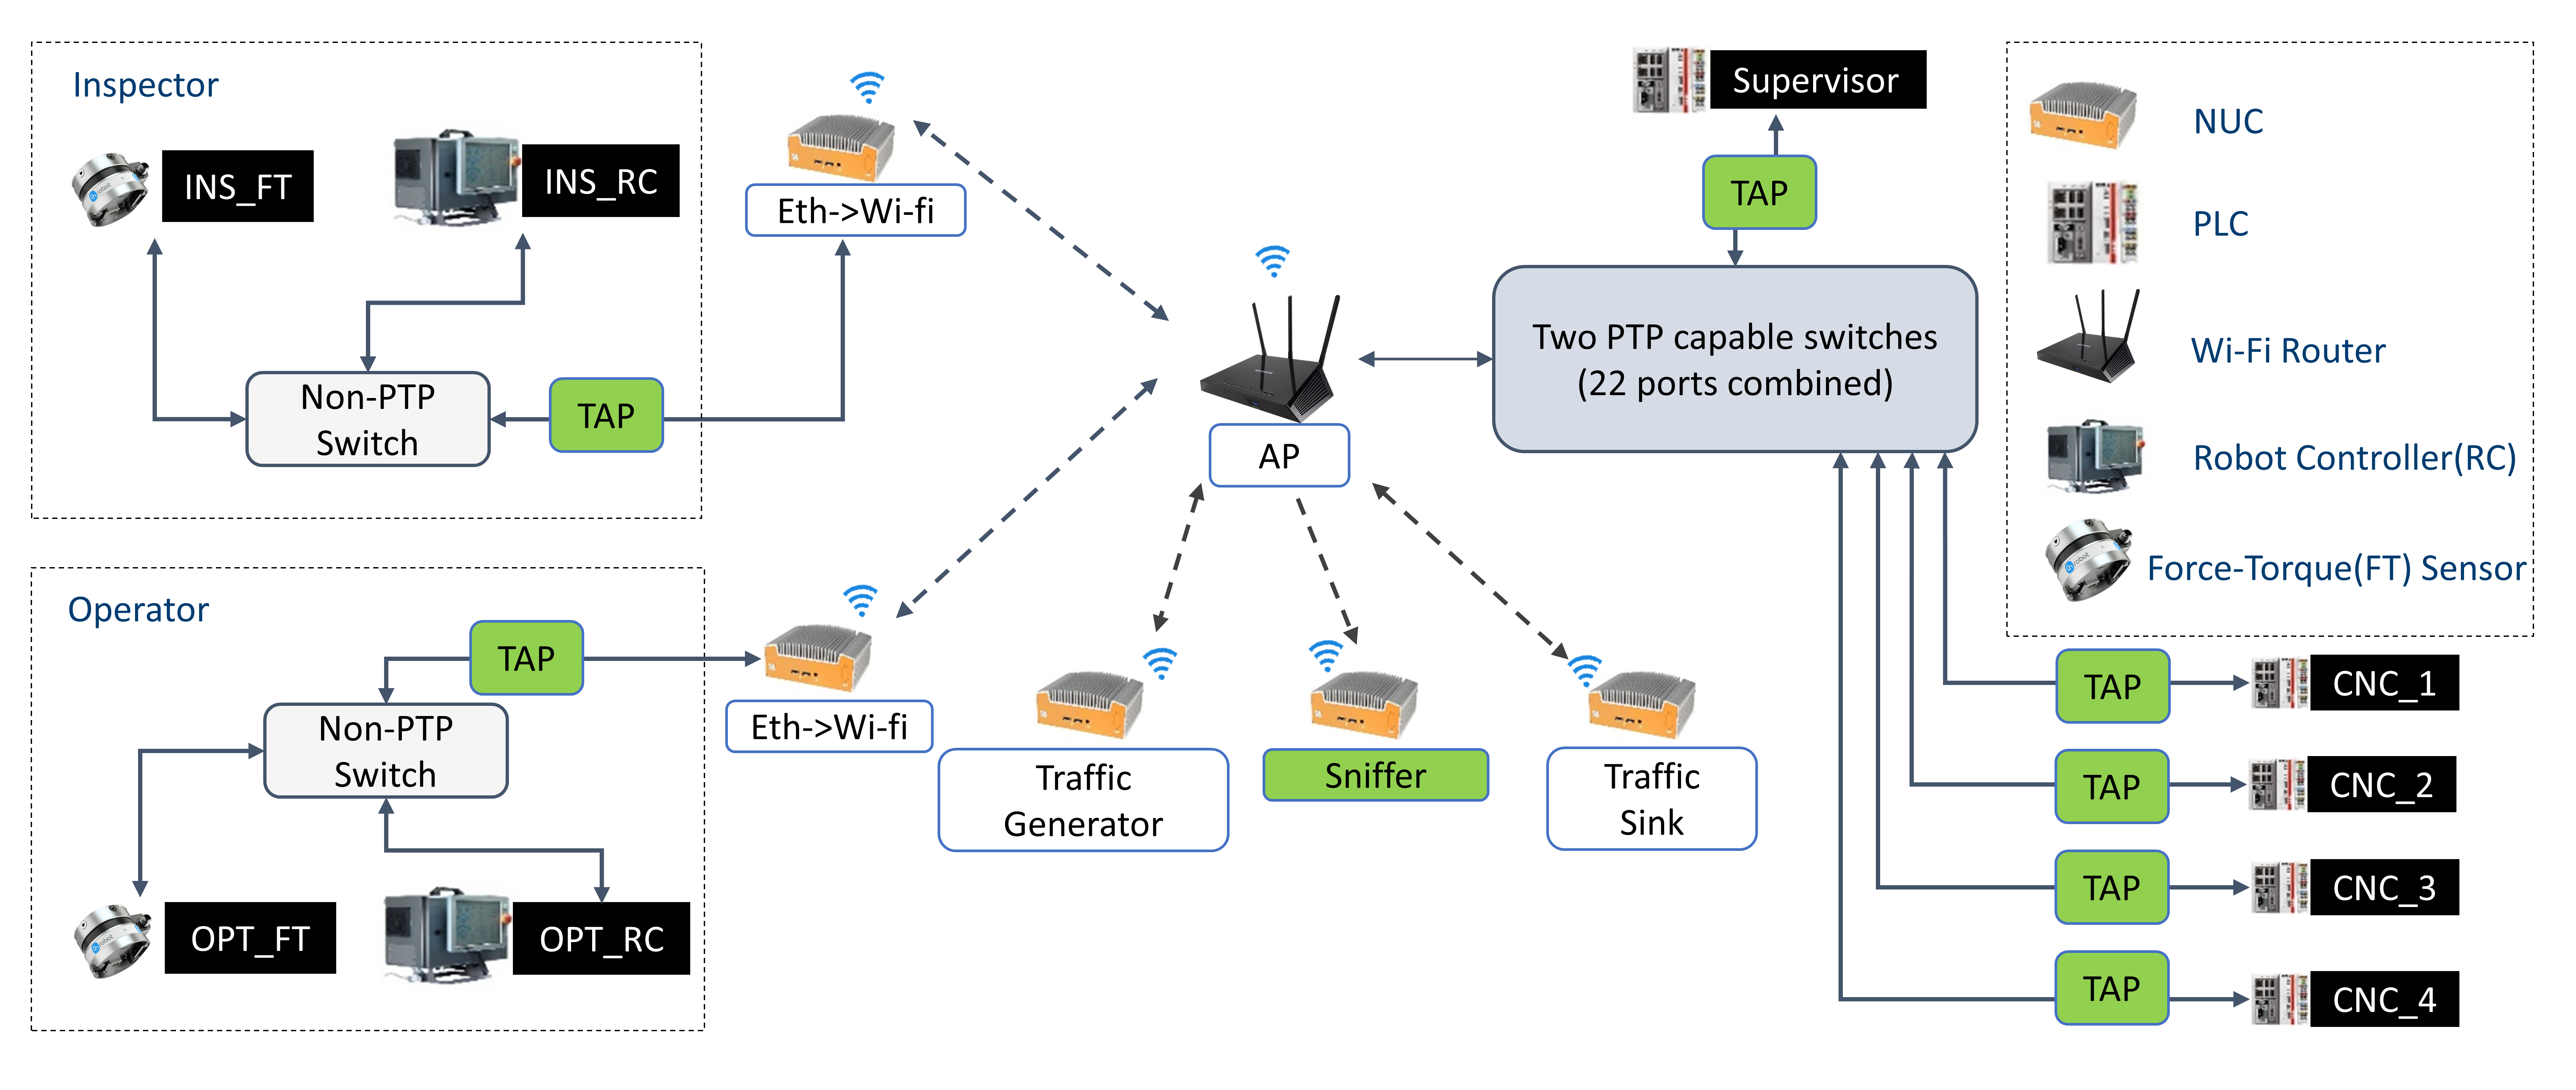
\includegraphics[width=\textwidth]{chapter-gdb-appl/figures/Fig1TiiSpecialDiagram-testbed2}
	\caption{Network diagram of the industrial wireless testbed at NIST. Solid lines represent Ethernet based communications and dashed lines represent wireless based communications.}
	\label{gdbappl:fig::database:netdiagram}
\end{figure*}

All communicating devices on the testbed have been originally designed to use Ethernet TCP/IP for communication. To enable wireless within the testbed, Ethernet-WiFi bridges are utilized for wireless communications through a common access point (AP). To establish these Ethernet-WiFi bridges, Next-line-of-Computing (NUC) computers, are used.  NUCs are a line of small-form-factor barebone computer kits designed by Intel.   Each NUC in our experiments is configured in one of various forms as a bridge, a wireless sniffer, a traffic generator, or a traffic sink. These configurations in the network are shown in Fig.~\ref{gdbappl:fig::database:netdiagram}.

There are three different types of measurements (network, robot, and PLC state data) collected on the testbed. Network traffic data is captured using seven test access point (TAP) devices and a wireless sniffer, shown in Fig.~\ref{gdbappl:fig::database:netdiagram} with green labels. A machine running Ubuntu 18.04, not shown, is used to capture all wired network traffic on the testbed. The position and robot state data is captured from the robot controllers using the real time data exchange (RTDE) protocol~\cite{RTDE}. RTDE data is also captured on the Linux machine using the connected switches to each of the robot controllers. Lastly, the PLC state data is captured locally on the supervisor PLC during the experiment. These three types of measurements (network, robot, and PLC state data) have a shared precise time from the synchronization to the grand master time server. The design adopts the IEEE 1588 precision time protocol (PTP) to allow synchronized distributed clocks to stamp the accurate time to the measured network and operational events in the testbed~\cite{IEEE-Std-1588-2008-redline}.

\subsection{Equipment Used}

The following equipment are illustrated in Fig.~\ref{gdbappl:fig::database:netdiagram} for reference.
To enable wireless on the testbed, Intel NUCs running Ubuntu 14.04 are used which communicate through a common AP. The AP is a Netgear AC1900 wireless router. For the wired communications, we use two Cisco IE 4000 industrial grade Ethernet switches that are PTP compatible for time synchronization. The collaborative robots that preform the pick and place task are Universal Robots “UR3” CB series. The robots are also equipped with OnRobot HEX-H Force/Torque sensors which are used by the Inspector to inspect parts. The Supervisor PLC is a Beckhoff CX2020 with a EL6688 PTP module for time synchronization. The CNC simulators are Beckhoff CX9020 PLCs. The seven TAP devices on the testbed are SharkTap Gigabit Network Sniffers. To synchronize the timing of the devices while taking measurements, a Meinberg Lantime M900 grand master time server is used. Lastly, the Operator and Inspector each use a D-link DGS-108 8-port unmanaged Ethernet switch for wired communications between the robot controller and force-torque sensor and for the Linux machine to collect RTDE data through a wired connection.

\subsection{Building the Graph} \label{gdbappl:sec:graph}

A GDB was built to manage data collected from testbed measurements of both network traffic and physical operations.
% Save for later -YL
%Compared with relational databases, GDBs as NoSQL databases don't specify any predefined data structure or rules to enforce such a structure. Instead, GDBs treat individual data records as distributed node entities in a random graph and identify relationships as part of database components that link different nodes together. This feature enables GDBs to catch varying states and dynamics in a complex system and gradually improve data management along with better understanding of the system.
In this section, we briefly introduce graph components developed for our testbed and the data processing flow that transforms measurement results to graph entities. 

\subsubsection{Reference Data Model}
%Save for later -YL
%In a GDB, the data model, which can be roughly analog to the ``schema'' of relational databases, illustrates how data records are organized and stored in a graph. However, unlike a fixed schema, the data model of GDBs has more flexibility of depicting diverse data types, content, and connections between different entities whose structure and property profile can update and evolve with more data and/or better observation. A data model contains different node types with specific properties in the graph and various relationships between them. 
In the previous case study, we identified the requirements of a GDB data model and built a graph containing nodes and relationships that mainly exhibit information around networked industrial devices in a factory workcell. In this continuation of the work, we further populate the earlier defined workcell data graph by introducing additional node types characterizing physical actions that are newly captured. Accordingly, we update the relationships, such as associating individual quality of service (QoS) report data from the wireless sniffer with the packets captured at the collocated receiver. The updated data model provides a comprehensive view of production operations, information flows, and wireless channel variations in the testbed which facilitates further analysis work.  

\begin{figure*}
	\centering
	%	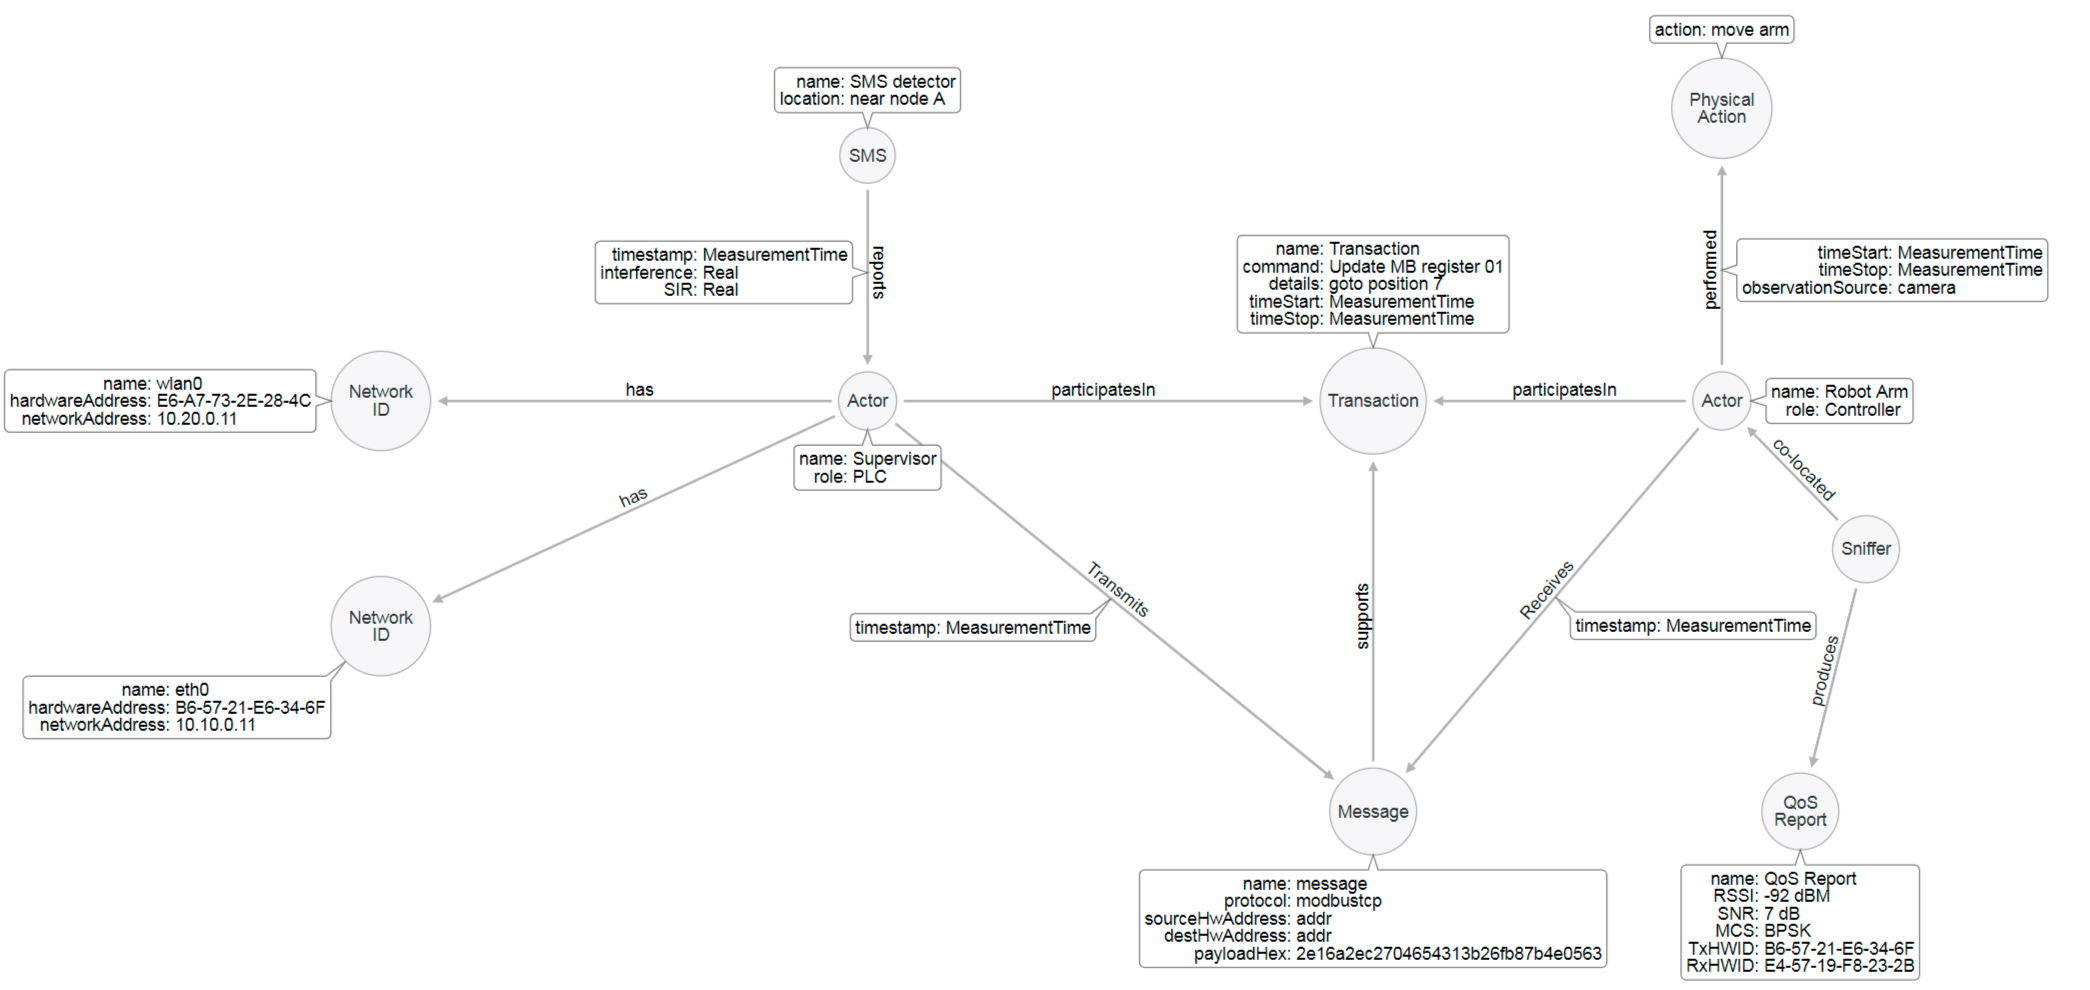
\includegraphics[width=\textwidth,trim=50 50 50 50, clip]{figures/database/arrows-schema.PNG}
	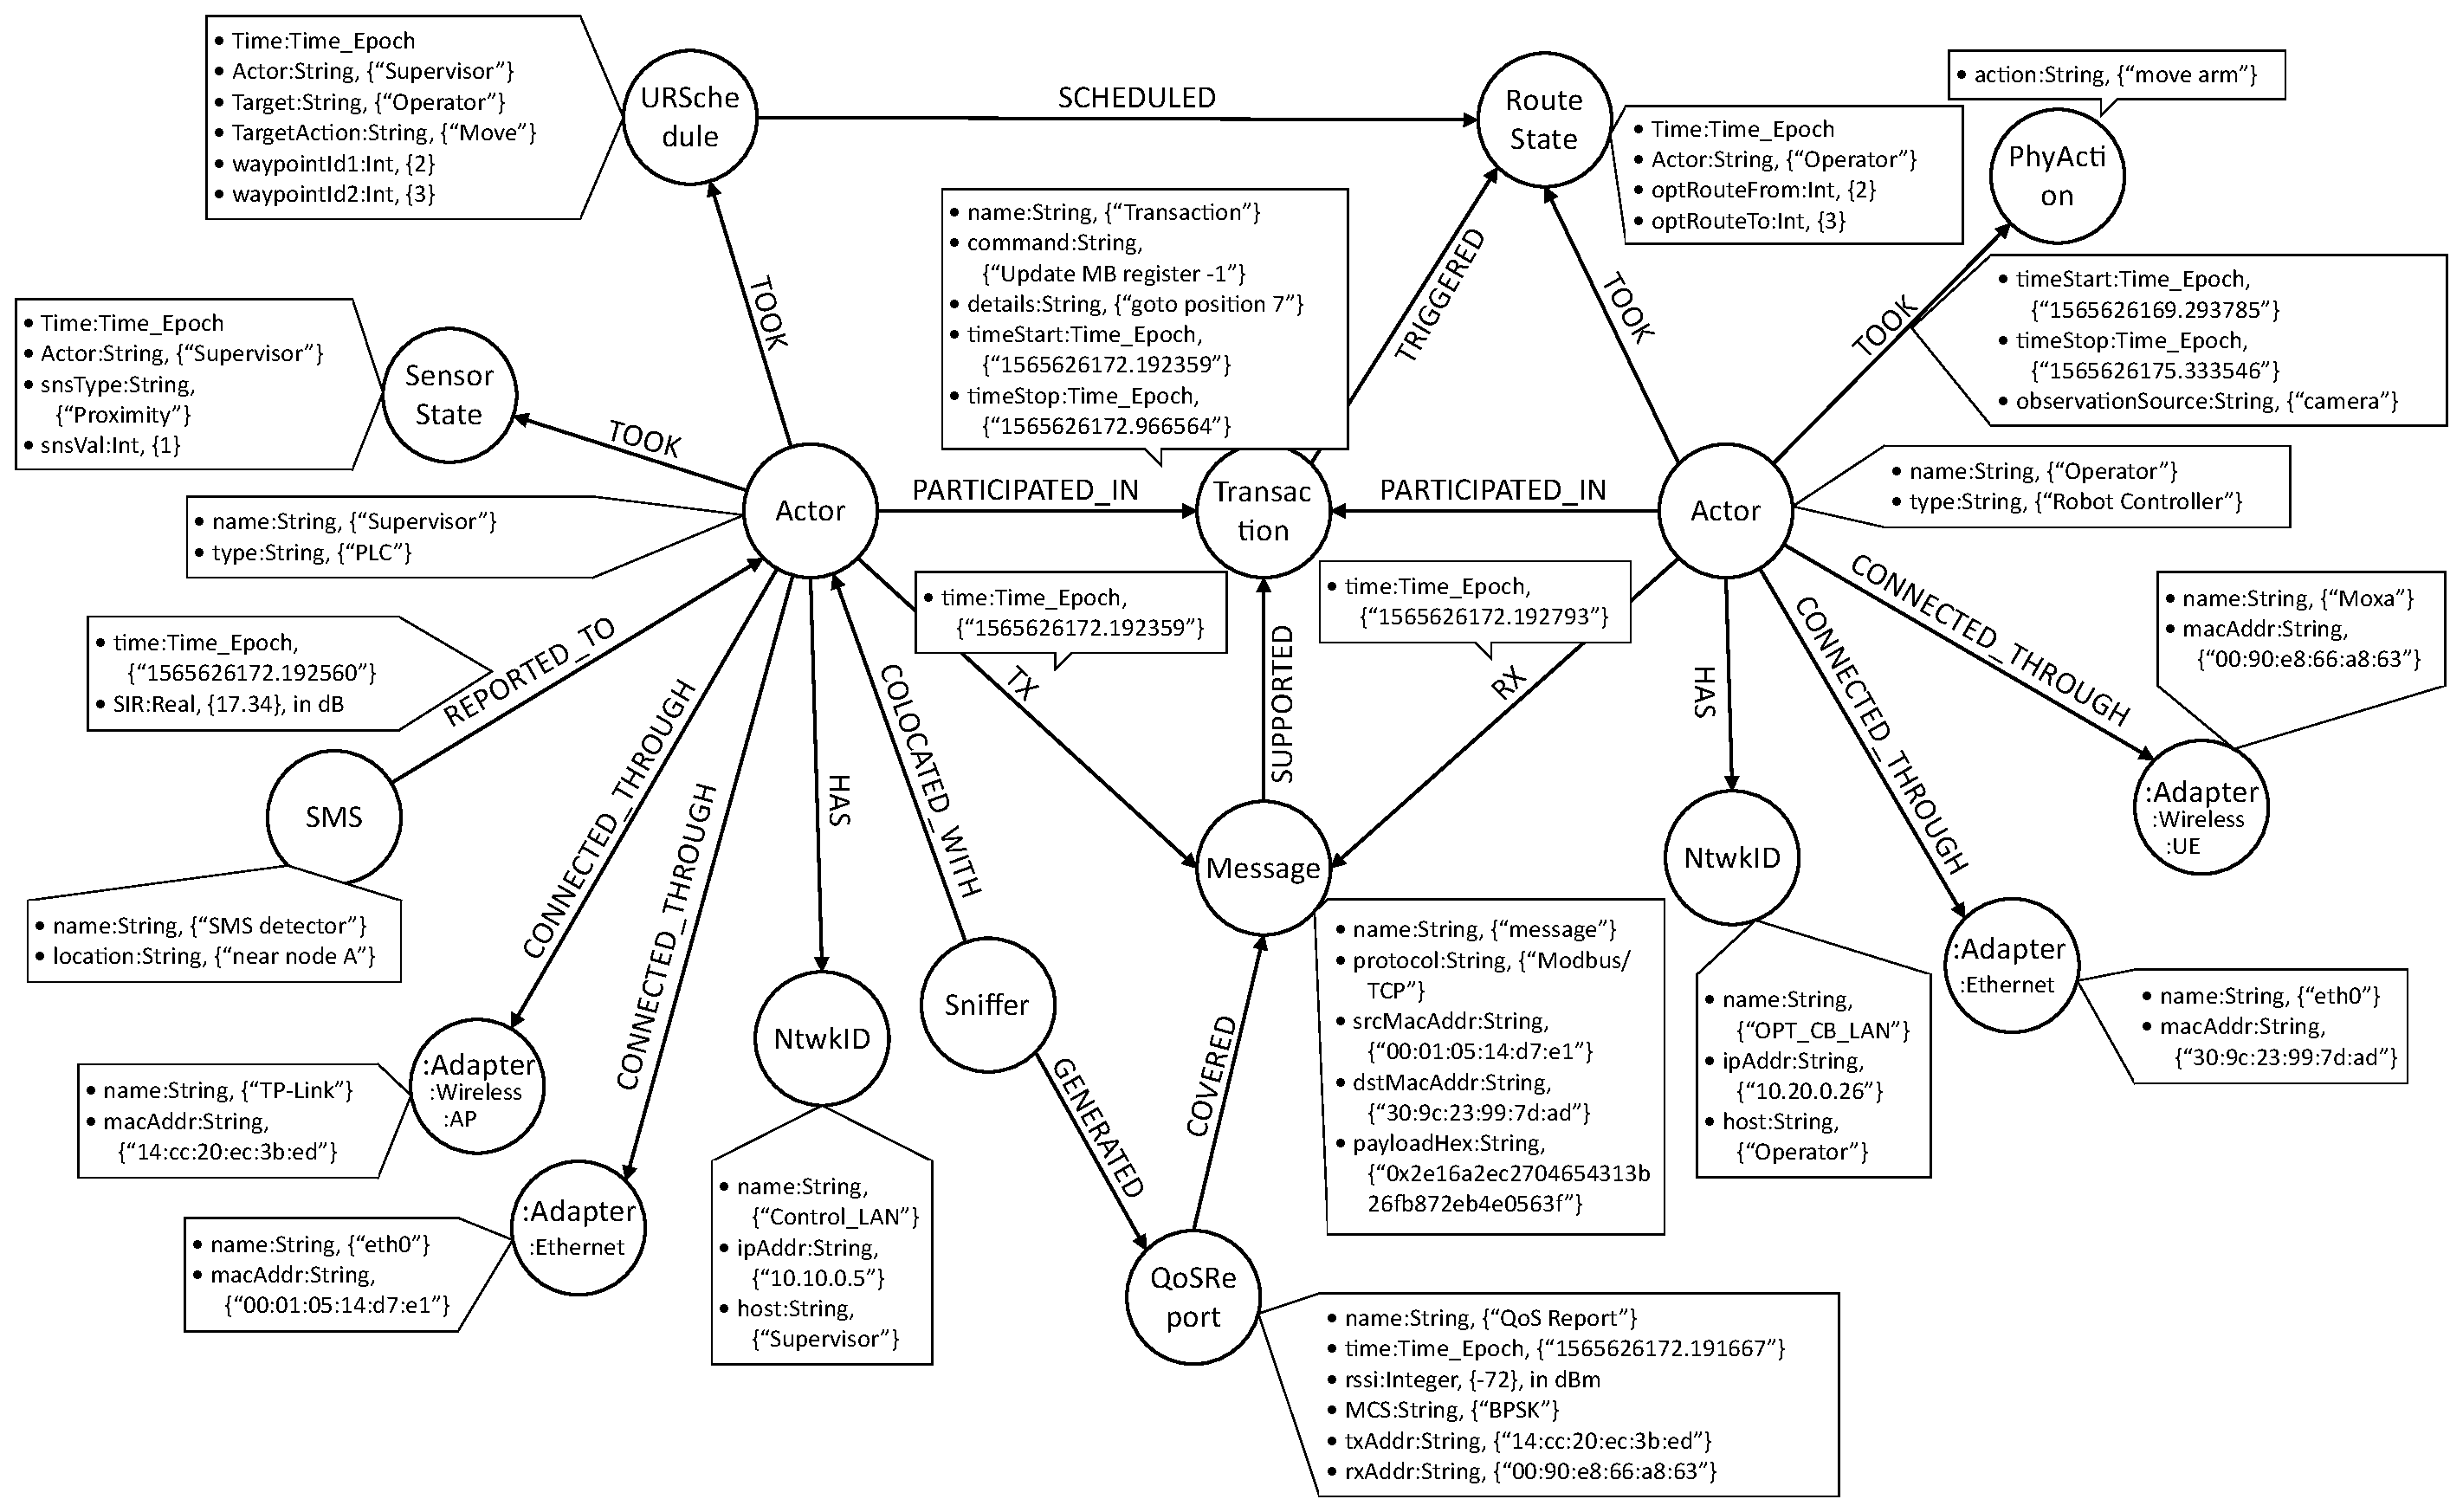
\includegraphics[width=\textwidth]{chapter-gdb-appl/figures/graph_schema_1209.eps}
	\caption{The data model of the graph database used for each operational run of the NIST wireless factory testbed.  The graph is organized into nodes and edges, where the edges signify relationships among network elements and physical operational elements.}
	\label{gdbappl:fig:database:schema}
\end{figure*}

As shown in Fig.~\ref{gdbappl:fig:database:schema}, an example is illustrated here that summarizes nodes, relationships, and their key properties used in the GDB. We will elaborate the definition and use of these entities in the remainder of this section.			


\paragraph{Node Design}

%To effectively depict testbed operations in the measurement, we define a series of node types in the graph. 
Nodes are GDB elements that are used to identify testbed components, device states, and messages that store snapshots of the testbed for further analysis. They can be found in two main classes depending on what type of objects the node represents.

The class of \textit{static} nodes covers testbed setup profiles which contain testbed components, network interfaces, and their settings. These entities are normally predetermined or collected in the initialization of each measurement. They usually remain constant in each round of measurements. This class includes Actor, Network ID (NtwkID), Spectrum Management System (SMS), Sniffer, and Adapter in the GDB. The Adapter nodes can further have additional labels to identify their network interfaces and the roles they play, such as Ethernet/Wireless and AP/user equipment (UE).

The class of \textit{dynamic} nodes in the graph captures various system events such as machine status reports, network traffic, and information flows in the testbed. These nodes are dynamically added into the graph whose quantities and properties are determined by the measured data. Such node labels include Transaction, Message, QoSReport, and Physical Action (PhyAction). Considering the diversity of measured testbed operations, PhyAction nodes have sub-class labels including URSchedule (for the Supervisor), SensorState (for CNC), and RouteState (for robots).


\paragraph{Graph Relationships}

A relationship in the graph denotes an action taken to associate two nodes, either homogeneous or heterogeneous ones, which shows their connections in the topology, timeline, or affiliation. The relationships used in the GDB were introduced in~\cite{CandellISIT2020.Conf}. As shown in Fig.~\ref{gdbappl:fig:database:schema}, most of them are self-explanatory. 

\begin{figure*}
	\centering
	%	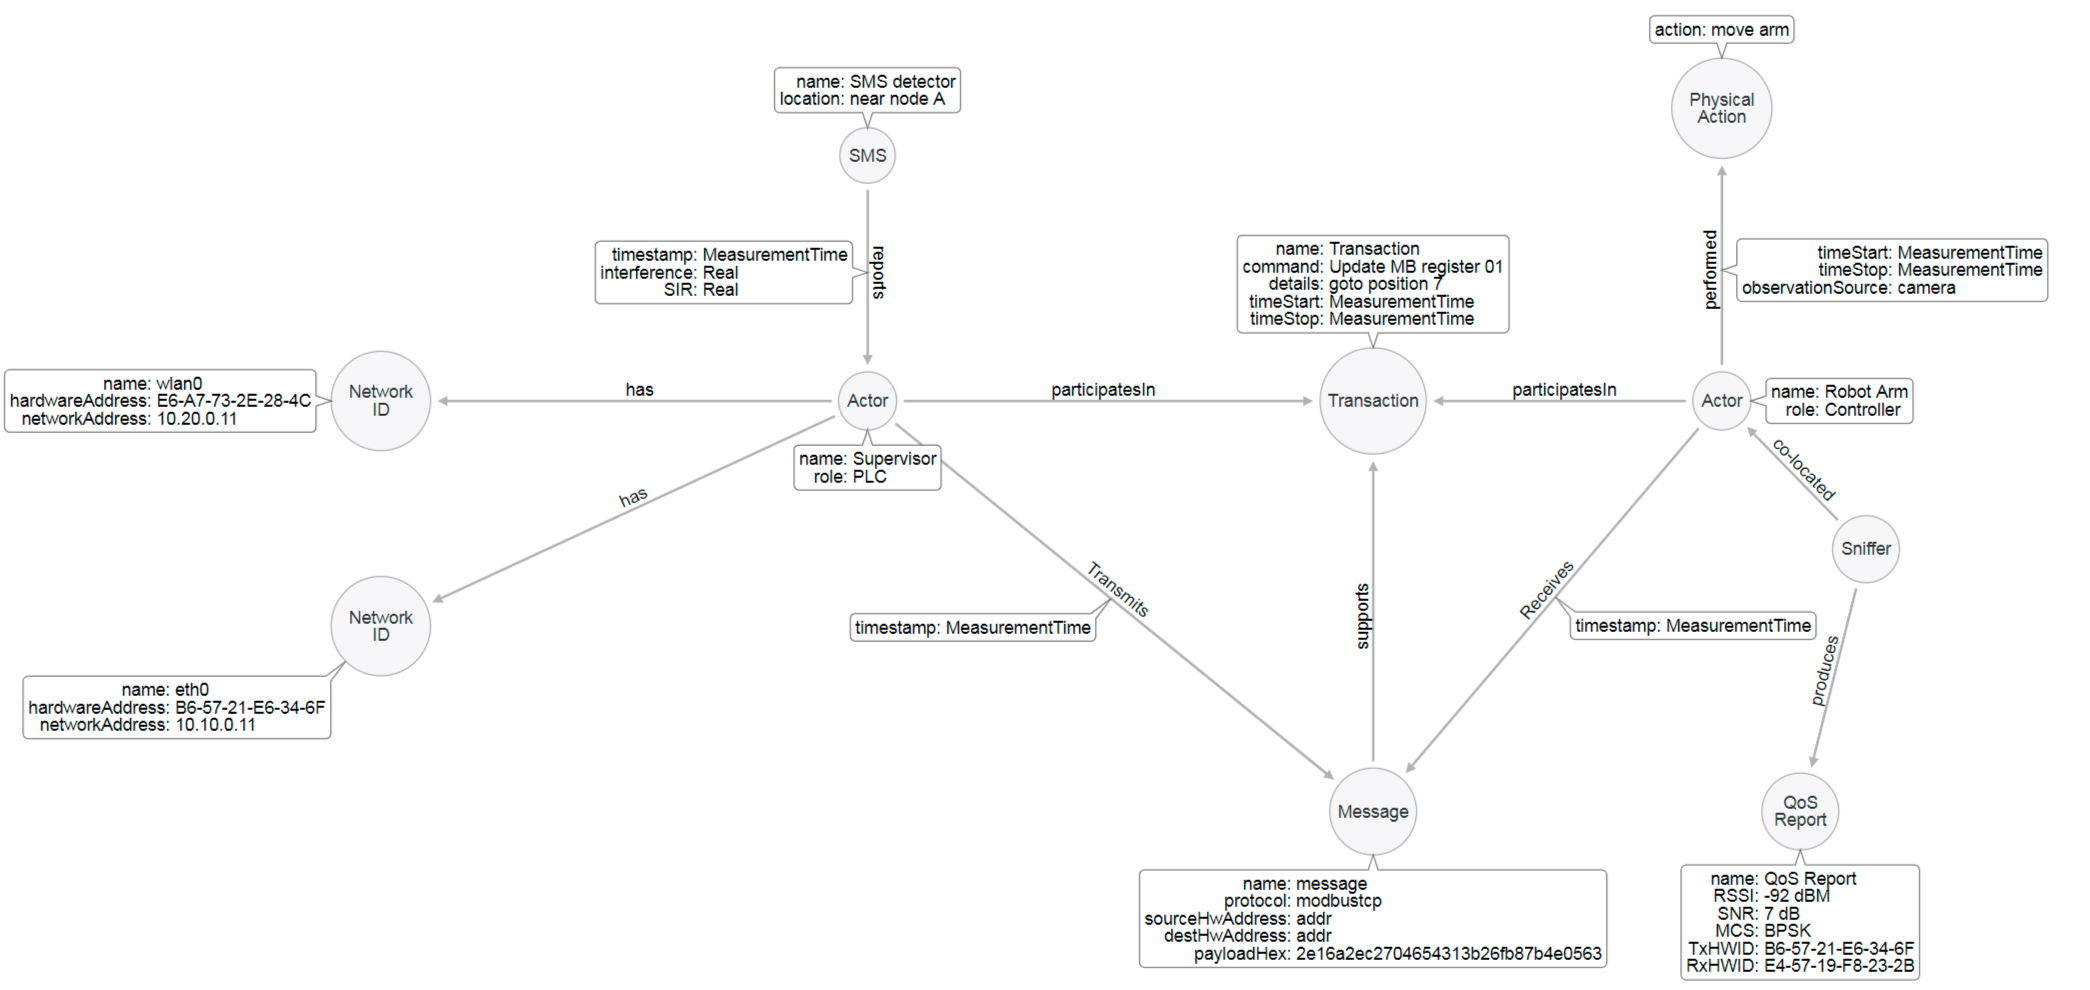
\includegraphics[width=\textwidth,trim=50 50 50 50, clip]{figures/database/arrows-schema.PNG}
	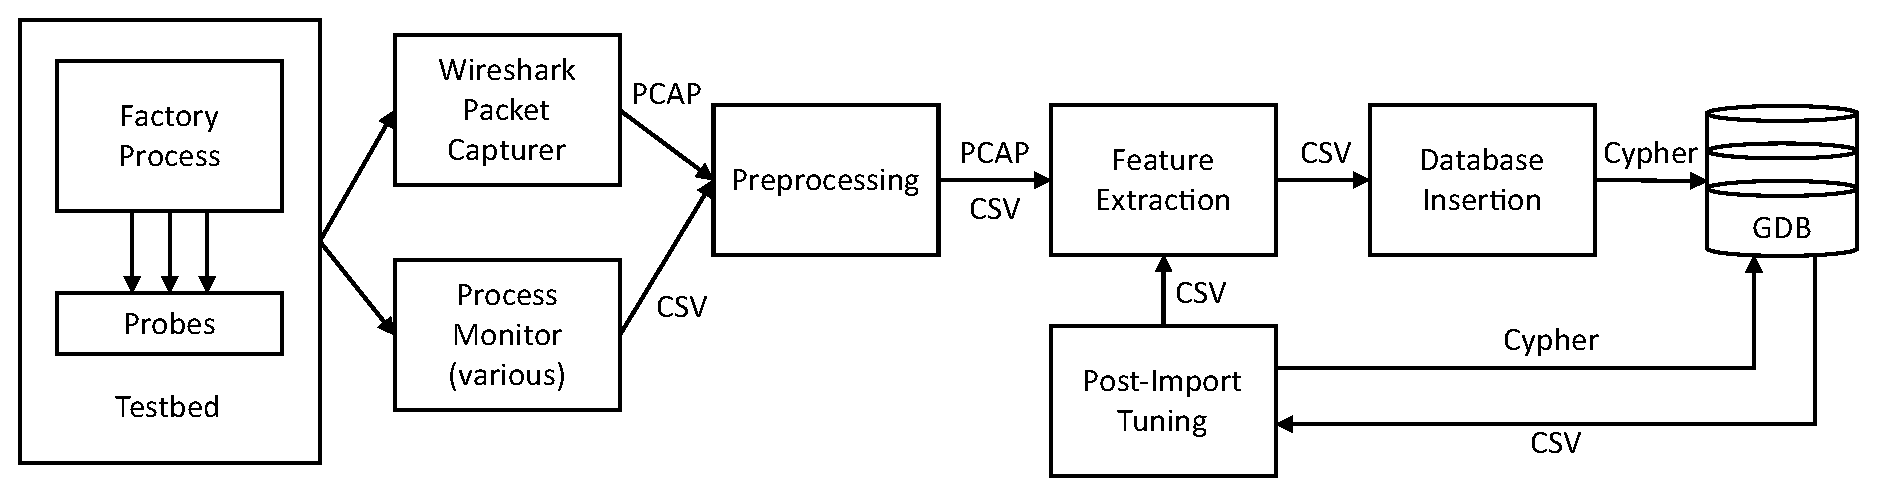
\includegraphics[width=\textwidth]{chapter-gdb-appl/figures/info_workflow_tii.eps}
	\caption{Data processing flow from factory workcell to database}
	\label{gdbappl:fig:database:work-flow}
\end{figure*}

\paragraph{Closer Examination}
The graph data model is designed in a way where nodes and relationships are centered around Actors. Actors have dual roles in the workcell operations. In the factory system, Actors participate in the production operations.
In the example of Fig.~\ref{gdbappl:fig:database:schema}, two Actor nodes are presented. In this case, Actor ``Supervisor'' is the supervisory controller, and Actor ``Operator'' is a robot arm. The Supervisor schedules the production, collects the other Actors' states, and hosts supportive services, such as SMS. The Operator follows the instructions of the Supervisor and moves parts between work stations. Meanwhile, Actors also act as communication nodes which exchange messages between each other through various network interfaces. In Fig.~\ref{gdbappl:fig:database:schema}, Actors participate in a transaction, which, in this example, is a Modbus/TCP exchange. The transaction itself is associated with one or more messages (i.e., packets). Each message associated with a transaction manifests itself as a node in the graph. Multiple message nodes will exist for each transaction. Additionally, QoS reports may be associated with each actor node through a collocated sniffer node.  %By keeping QoS reports separate, we have the flexibility of supporting different wired and wireless protocols within the same graph.

Dynamic event nodes in the measurement, i.e., physical actions, network messages, information transactions, and QoSReport records, have timestamps representing ``measurement time'' of the recorded events. Once a new event occurs, a proper relationship would be added between the actor and the physical/network event node. All timestamps are accurately synchronized to the grand-master clock.


\subsubsection{Information Workflow}

A multi-stage workflow is deployed to feed the graph with instances of nodes, relationships, and their properties that are extracted from measurement data, as shown in Fig.~\ref{gdbappl:fig:database:work-flow}. In the measurement data set, network data from distributed network probes in selected links is stored in packet capture (PCAP) files, while operational data that comes from different PLC and robot controllers is stored in the format of comma separated value (CSV) files. The whole process contains four steps including data preprocessing, feature extraction, database insertion, and post-import tuning. Such conversion from raw data to the ready-to-go graph has been done  by running automated scripts on a host machine which maintains data repositories of measurement results and deploys the Neo4j desktop application. The functions and operation features in individual steps are discussed next. 


\paragraph{Data Preprocessing}

Data preprocessing is the first step where measurement data is verified, cleaned, and formatted to facilitate the following processing steps. As fore-mentioned, measurement data contains results collected from heterogeneous modules/devices in the testbed which may adopt different data types, sampling rates, time and metric resolution, and file formats. For example, different machines may represent and store the record timestamps in various formats depending on local clock settings. Once we obtained the data, we unified the time representation in the entire data set using the time epoch that has microsecond resolution. In another example, we deployed packet filters to remove unrelated packet captures. In treating measurement data, e.g., experimenting with single or double wireless interference links, we managed to reduce the sniffer data in the order of gigabytes to only a few megabytes while keeping all signaling handshakes of interest in the studied links. 

\paragraph{Feature Extraction}

Feature extraction refers to the process of extracting relevant information from measurement data and prepare the data for insertion into the database. Nodes and relationships are defined by a set of features that share common views. We developed bash and Python scripts that pick the desired features to produce CSV files that are ready for insertion into the Neo4j database. In this step, a bash script was developed running the tshark tool to extract fields of protocol headers in packet captures and save the field information into CSV files. Each line in these CSV records will create one Message node instance as a sender or receiver copy of the packet through a link. A Python script was also used to detect state switches in the physical action data and label these moments which were triggered by testbed communications.


\paragraph{Graph Insertion}

We load the prepared data into the Neo4j GDB using bulk importing which can create one or multiple nodes and/or relationships in the graph by reading a CSV file once. 
Neo4j uses Cypher to construct GDB queries to import data.
As the output of feature extraction, each line of the CSV file can create one new node entity and/or generate the criteria of linking two qualified nodes for a new relationship. Properties of new entities can be assigned explicitly by the column values of records or inferred from predetermined rules such as some fixed combination of nodes and edges in the graph. Multiple types of nodes can be created from the same data file using one common node template in which each node type has its own subgroup of properties. For example, Modbus and ADS packets use the same Message node structure in our graph to manage the common transmission information such as IP addresses and TCP session identification. Meanwhile, each of these Messages maintains its own application layer header information in the node properties, e.g., Modbus register addresses and ADS function codes.   


\paragraph{Post-Import Tuning}

Post-import tuning refers to any additional modification in the graph after CSV data is imported. This step treats a few cases where raw data work with current graph insights to obtain new ones. First, in the additive insertion case, i.e., when new data is added into the graph, it links the newly added nodes to the existing ones following necessary relationships between them. Time series data often use this method to link consecutive event nodes in the recorded process.
Second, it is the case in which higher level features are needed in the graph which can be abstracted from the imported data. For example, Transaction nodes are built upon Message nodes who participate in the same application transactions; Message nodes themselves are also the summary of packet data, i.e., packet copies at link transceivers. Third, it can feed feature extraction with pieces of information in the current graph for purposes such as coupling data records. For example, coupling QoS reports and Messages in their observation windows used to be an extremely time-consuming process. On one hand, each Message raw data, i.e., the transmitter or receiver copy, contains only half of the transmission time window information. On the other hand, the Cypher query takes a long time to find all eligible relationships as Neo4j would generate a huge Cartesian product when treating the large sample set. We solved this issue by obtaining qualified Message nodes and feeding them into feature extraction where a more efficient Python script finds all Message-QoS Report pairs and later presents them in the graph as new COVERED relationships. 


The above four steps can perform multiple iterations to treat data and refine the graph according to the data complexity and requirements.  
%
\begin{figure*}
	\centering
	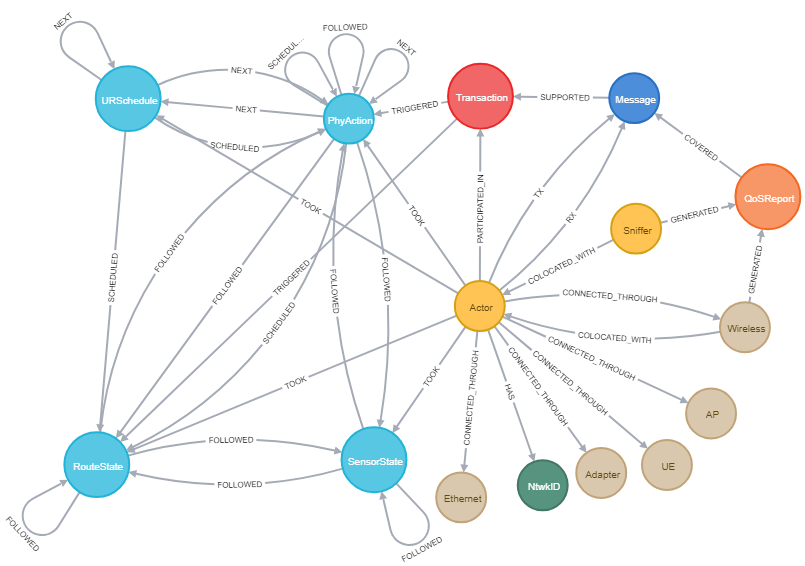
\includegraphics[width=0.8\textwidth,height=3.5in]{chapter-gdb-appl/figures/database/graph_schema_updated_2.png}
	\caption{Realized schema of the graph database fully populated after capturing network and operational data from the NIST industrial wireless testbed. \vspace{-0.2in}}
	\label{gdbappl:fig:real-schema}
\end{figure*}

\subsection{Results} \label{gdbappl:sec:results}

Once the data resides within the database, we apply queries to extract information for the evaluation of workcell performance and visualization of network and operational events within the workcell. By tracking paths through the relationships within the graph, discerning how a network event such as interference relates to physical events such as position uncertainty or part throughput is possible. Various impairments may be introduced as a part of workcell operation.  Examples of such impairments include competing wireless traffic, radio interference, and reflections and diffraction due to the multi-path environment~\cite{Candell2017.NIST1951}. We have shown that it is feasible to implement such impairments and measure the resulting physical performance manifestation~\cite{Liu2019vancouver}. 


In the following, we show results from an experimental scenario of the NIST industrial wireless testbed. In this scenario, two wireless links are used to connect the robot controllers and the wireless AP that is connected to all the other actors in the testbed. The wireless nodes are IEEE 802.11b/g/n devices. During each run of this experimental scenario, the production of 20 parts was emulated, which resulted in 12 minutes of network activity. We performed 4 different experimental cases with respect to the communications network, namely, 1) wired baseline where all links are connected using Ethernet cables to act as a benchmark for performance comparison, 2) wireless baseline where the robots traffic is the only traffic transferred over the wireless network, 3) with 2500 packets per second (pps) wireless traffic where a pair of a source and a sink operate simultaneously with the robots traffic over the wireless network, and 4) with 2x1250 pps traffic where two communications pairs of a source and a sink that each source generates 1250 pps traffic simultaneously with the robots traffic. These external traffic pairs have packet size of 1000 Bytes.        
\subsubsection{Realized Schema}

After populating the database with data captured from the experiment runs, the resulting realized schema is shown in Fig.~\ref{gdbappl:fig:real-schema}. The schema visualization is produced by invoking the command

\begin{lstlisting}
call db.schema.visualization()
\end{lstlisting} 
in Neo4j. It is important to note that, in comparison to the data model shown in Fig.~\ref{gdbappl:fig:database:schema}, a realized schema shows only one representation of each node and relationship . Where label inheritance is employed, such as the case for different adapter types, relationships are reproduced; however, this is a result of the visualization tool rather than the schema itself. Fig.~\ref{gdbappl:fig:real-schema} serves, therefore, to validate that the intended data model was indeed realized by the insertion of event data from the testbed. In the realized schema, inherited labels are shown as separate nodes.

% As described in Section~\ref{gdbappl:sec:dbschema}, the database includes every network transaction that occurs during operation of the testbed.  This includes any logical transaction nodes inserted into the database and any associated packets that happened to traverse the network.  Therefore, for a short duration of time depending on packet transmission rates, the amount of data stored in the database can grow quickly. This presents a visualization challenge that graphs are designed to handle. A sample graph is shown in Fig.~\ref{fig:Sample-graph_1}, which represents only 1 second of wired and wireless network data captured from the NIST two-robot pick-and-place wireless testbed described in~\cite{Liu2019vancouver}. 

% \begin{figure}
%     \centering
%   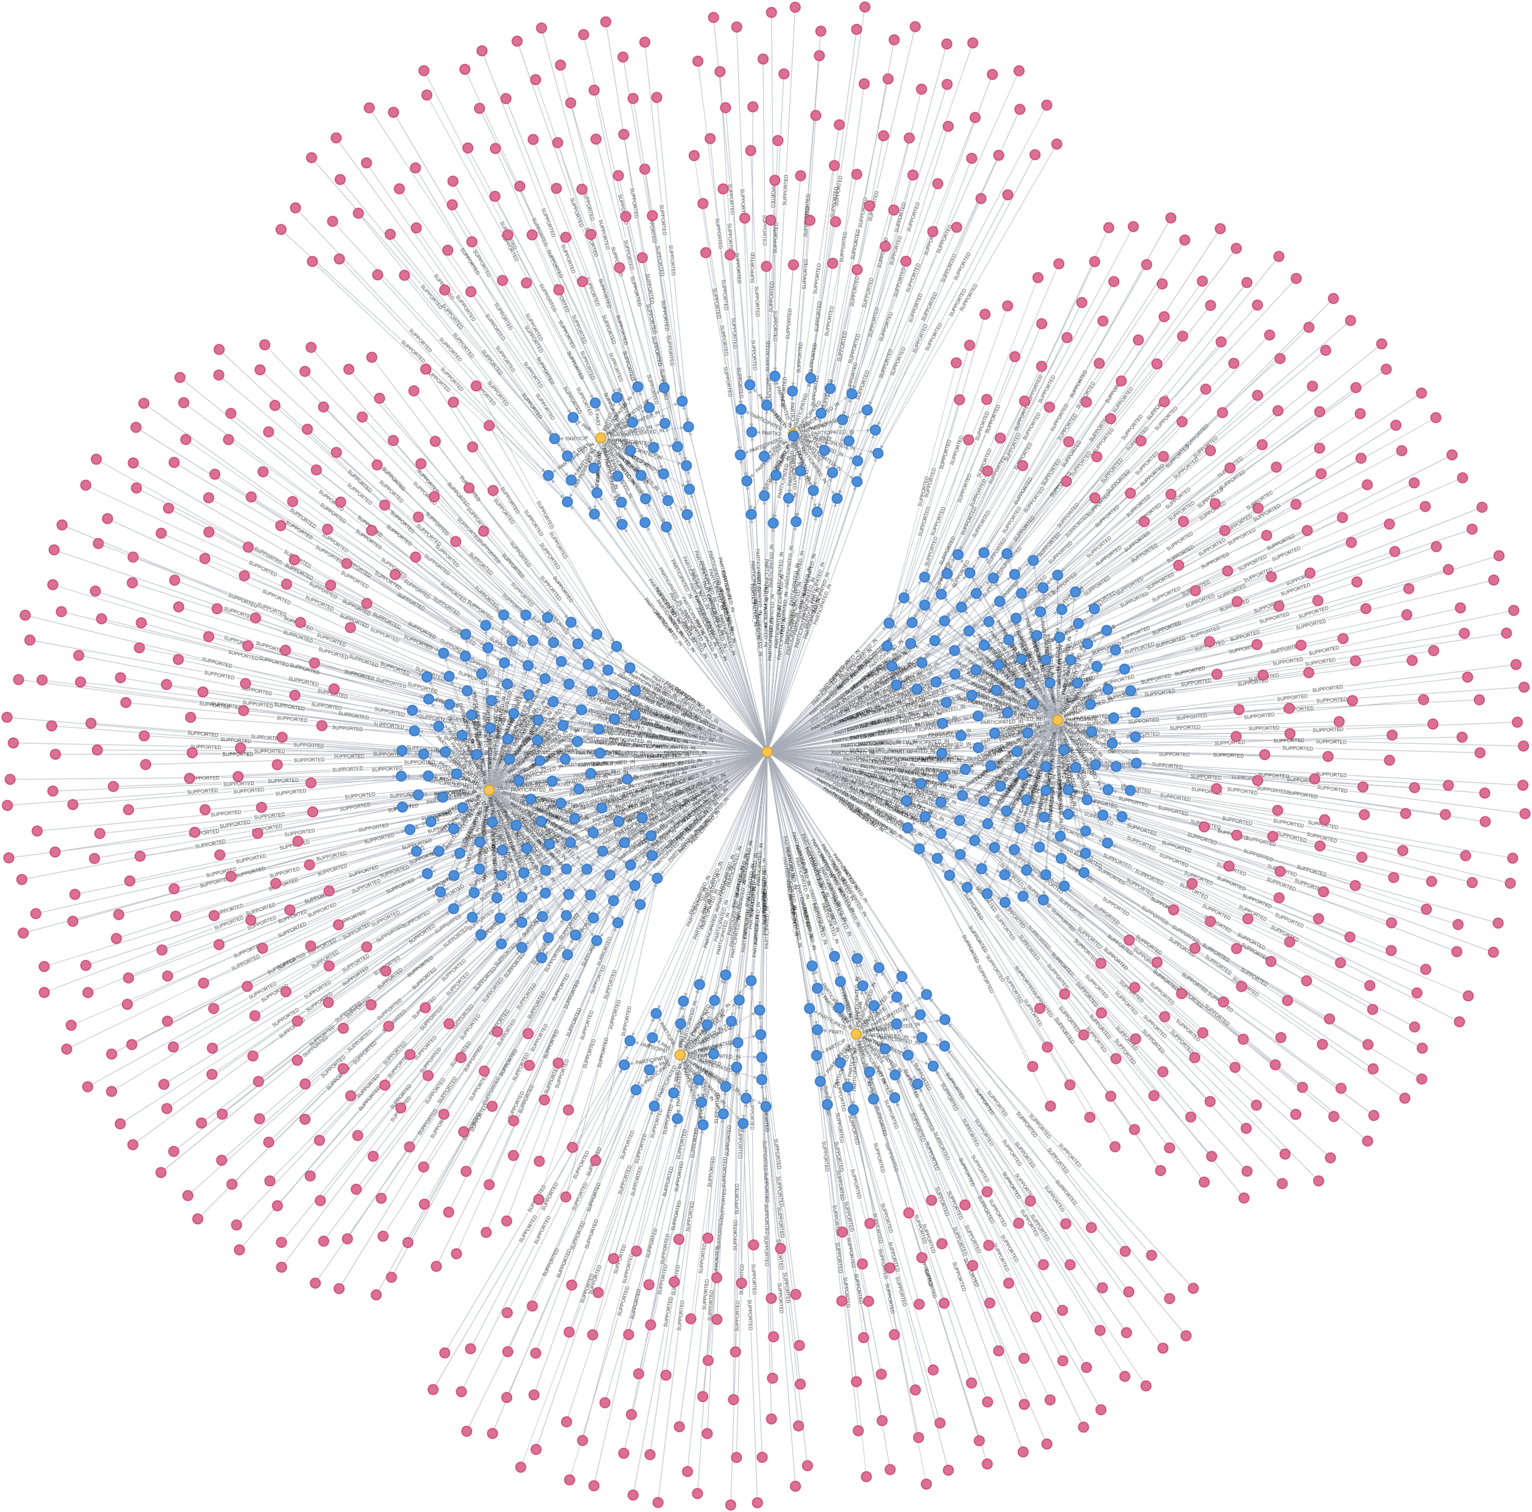
\includegraphics[width=0.49\textwidth]{figures/database/graph_M_T_2.png}
%     \caption{Visualization of a node graph resulting from a testbed experiment. }
%     \label{fig:Sample-graph_1}
% \end{figure}

% This visualization is produced by calling the following query in the Neo4j. 
% \begin{lstlisting}
% MATCH p=(a:Actor {name:'Supervisor'})--(t:Transaction)--(b:Actor) ,p2=(m:Message)-->(t) WHERE t.timeStart>T AND t.timeStop<T+1
% RETURN p,p2
% \end{lstlisting}

% The colors of the resulting nodes follow the realized schema in Fig.~\ref{fig:real-schema} while only the actors, transactions, and messages are visualized in~\ref{fig:Sample-graph_1}. The relationships between the messages and transactions are shown where a single transaction is connected to at least two messages to represent the communications between any two actors. The variable T in the query represents an arbitrary time variable in seconds within the trial run to capture the data within 1 second only.

% We then show a more detailed visualization for all the nodes and relationships corresponding to a single transaction. This visualization is produced by calling the following query where Ts is an arbitrary time variable to specify the timeStart value for the single transaction. 

% \begin{lstlisting}
% MATCH p=(a:Actor {name:'Supervisor'})-->(t:Transaction {timeStart:Ts})<--(b:Actor {name:"CNC-1"})
% WITH p, a, b, t
% MATCH p1=(a)-->(m:Message)<--(b), p2=(m)-->(t), p3=(a)-[:HAS]-(),p4=(a)<-[:COLOCATED_WITH]-()-[:PRODUCED]->(q:QoSReport), p5=(a)-[:CONNECTED_THROUGH]-(),p6=(b)-[:HAS]-(), p7=(b)-[:CONNECTED_THROUGH]-()
% WHERE q.time>t.timeStart AND q.time<t.timeStop
% RETURN p,p1,p2,p3,p4,p5,p6,p7
% \end{lstlisting}

% In Fig.~\ref{fig:Sample-graph_2}, the actor nodes are labeled by their names \textit{CNC-1} and \textit{Supervisor}, the transaction is labeled by its type \textit{ADS}, the messages are labeled by their transmission role \textit{Request} and \textit{Response}, the NtwkIDs are labeled by their IP addresses, the Ethernet adapters are labeled by their names \textit{eth0}, the wireless adapters are labeled by their names \textit{Moxa} and \textit{TP-Link}, the sniffer is labeled by its name \textit{WLS1}, and the QoS reports are labeled by the received signal strength indicator (RSSI) value in dBm. This visualization includes only the QoS reports generated within the duration of the corresponding transaction.   

% \begin{figure*}[!h]
%     \centering
%     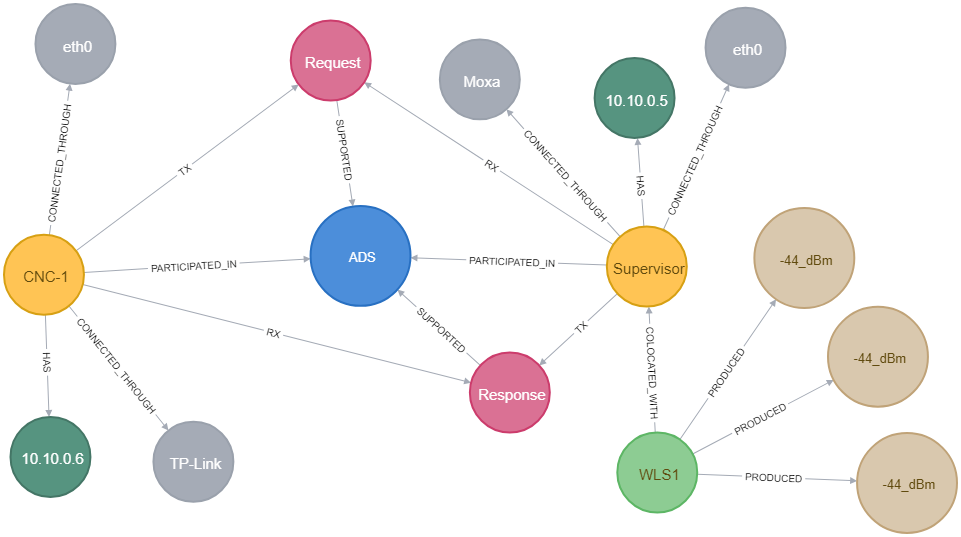
\includegraphics[width=0.8\textwidth]{figures/database/graph_Single_trans.png}
%     \caption{A detailed visualization resulting from a testbed experiment for all the nodes and relationships corresponding to a single transaction. }
%     \label{fig:Sample-graph_2}
% \end{figure*}

\subsubsection{Physical Actions Processing}
In this subsection, we use the extracted data from the GDB to study the impact of the wireless communications on the physical action performance. We focus our analysis in this subsection on the URSchedule and RouteState progress over time where URSchedule is the dynamic node to represent a physical action decision at the supervisor and RouteState is the dynamic node to represent a physical action command received by one of the robots where the command parameters are stored at the robot registers. Note here that the transaction between a robot controller and the supervisor is initiated by a request message from the robot controller and terminated by correctly receiving a response message from the supervisor to the robot controller as well. 

The Supervisor takes decisions based on available information about the testbed. Once it makes a decision, it is reflected on the value of the URSchedule. We define the Supervisor processing time as the time from the instant the decision is taken to the instant when the wireless transaction is initiated to request a new physical action and it is denoted by $T_\text{Sup}$. Then, the transaction latency is the time between the instant the wireless transaction is initiated by the robot to require a new action till it is the data is received at the intended robot controller and it is denoted by $T_\text{W}$. The robot processing time is the time between the instant the wireless data is received by the robot to the instant where the RouteState register is updated to reflect the required action and hence the physical action starts. The robot processing time is denoted by  $T_\text{Rob}$.  
The total physical action time which represents the time needed for a supervisor command to be reflected at the corresponding robot is denoted by $T_\text{Act}$ and evaluated through
\begin{equation}
T_\text{Act}=T_\text{Sup}+T_\text{W}+T_\text{Rob}.
\end{equation}

In Fig.~\ref{gdbappl:fig:database:Time}, we present the values of the three components of the action processing time for each run of the testbed. The horizontal axis represents the action index for all the Operator and Inspector actions while the corresponding time components are shown in the vertical figure axis. 

% \begin{figure}
% 	\centering
% 	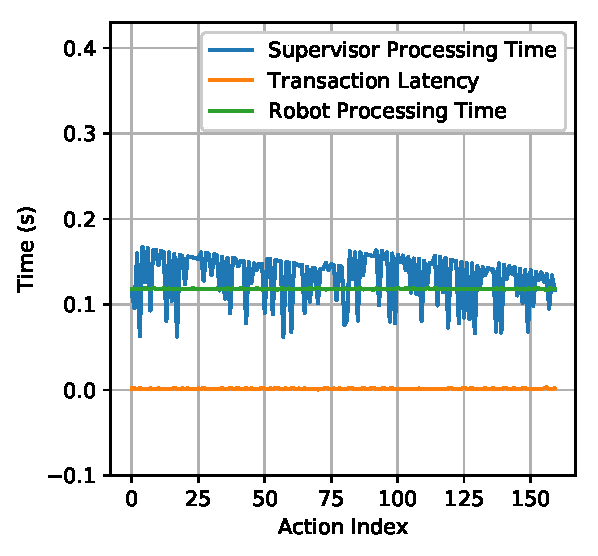
\includegraphics[width=0.45\textwidth]{figures/database/WiredBaseline_Time_Components_1.eps}
% 	\caption{Wired baseline action processing time.}
% 	\label{fig:database:Time_Wired}
% \end{figure}

% \begin{figure}
% 	\centering
% 	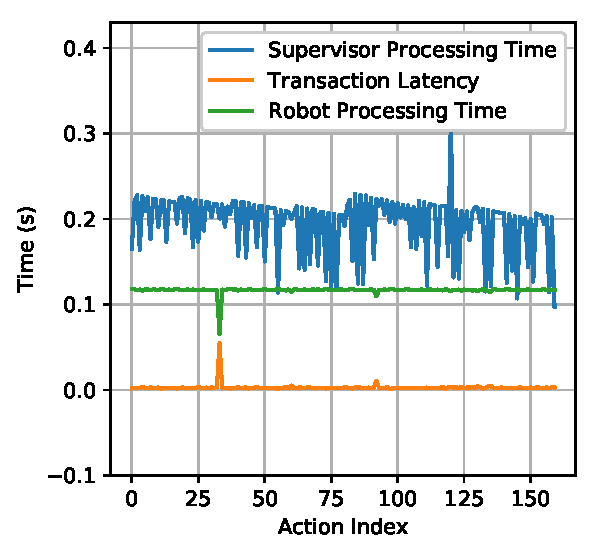
\includegraphics[width=0.45\textwidth]{figures/database/WirelessBaseline_Time_Components_1.eps}
% 	\caption{Wireless baseline action processing time. .}
% 	\label{fig:database:Time_Wireless}
% \end{figure}

% \begin{figure}
% 	\centering
% 	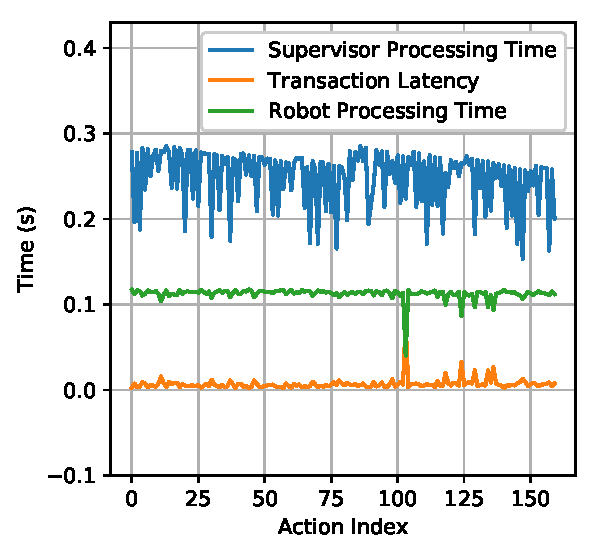
\includegraphics[width=0.45\textwidth]{figures/database/2500pps1000Bv1_Time_Components_1.eps}
% 	\caption{Wireless with 2500 packets/s traffic action processing time (first run).}
% 	\label{fig:database:Time_2500v1}
% \end{figure}

% \begin{figure}
% 	\centering
% 	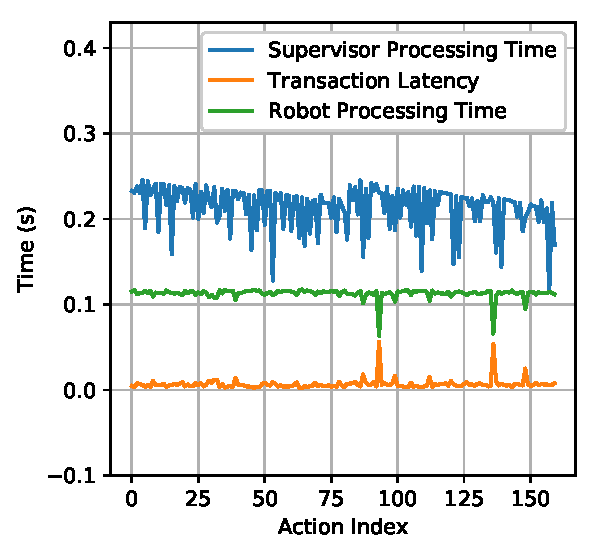
\includegraphics[width=0.45\textwidth]{figures/database/2500pps1000Bv2_Time_Components_1.eps}
% 	\caption{Wireless with 2500 packets/s traffic action processing time (second run).}
% 	\label{fig:database:Time_2500v2}
% \end{figure}

% \begin{figure}
% 	\centering
% 	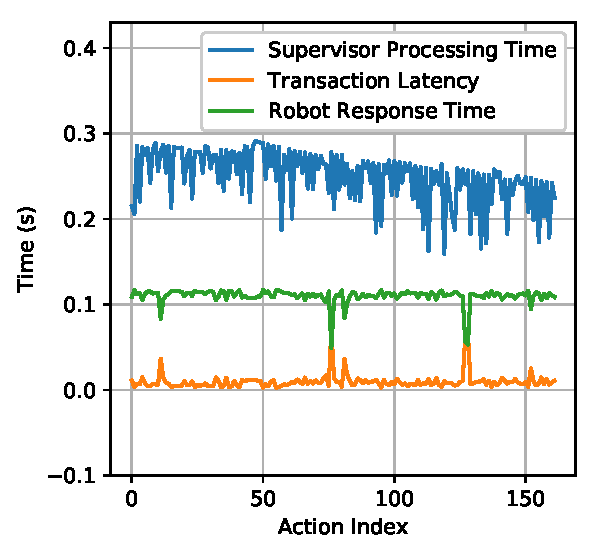
\includegraphics[width=0.45\textwidth]{figures/database/2X1250pps1000Bv1_Time_Components_1.eps}
% 	\caption{Wireless with 2x1250 packets/s traffic action processing time.}
% 	\label{fig:database:Time_2x1250}
% \end{figure}

\begin{figure}[!ht]
	\centering
	\subfloat[Wired Baseline]{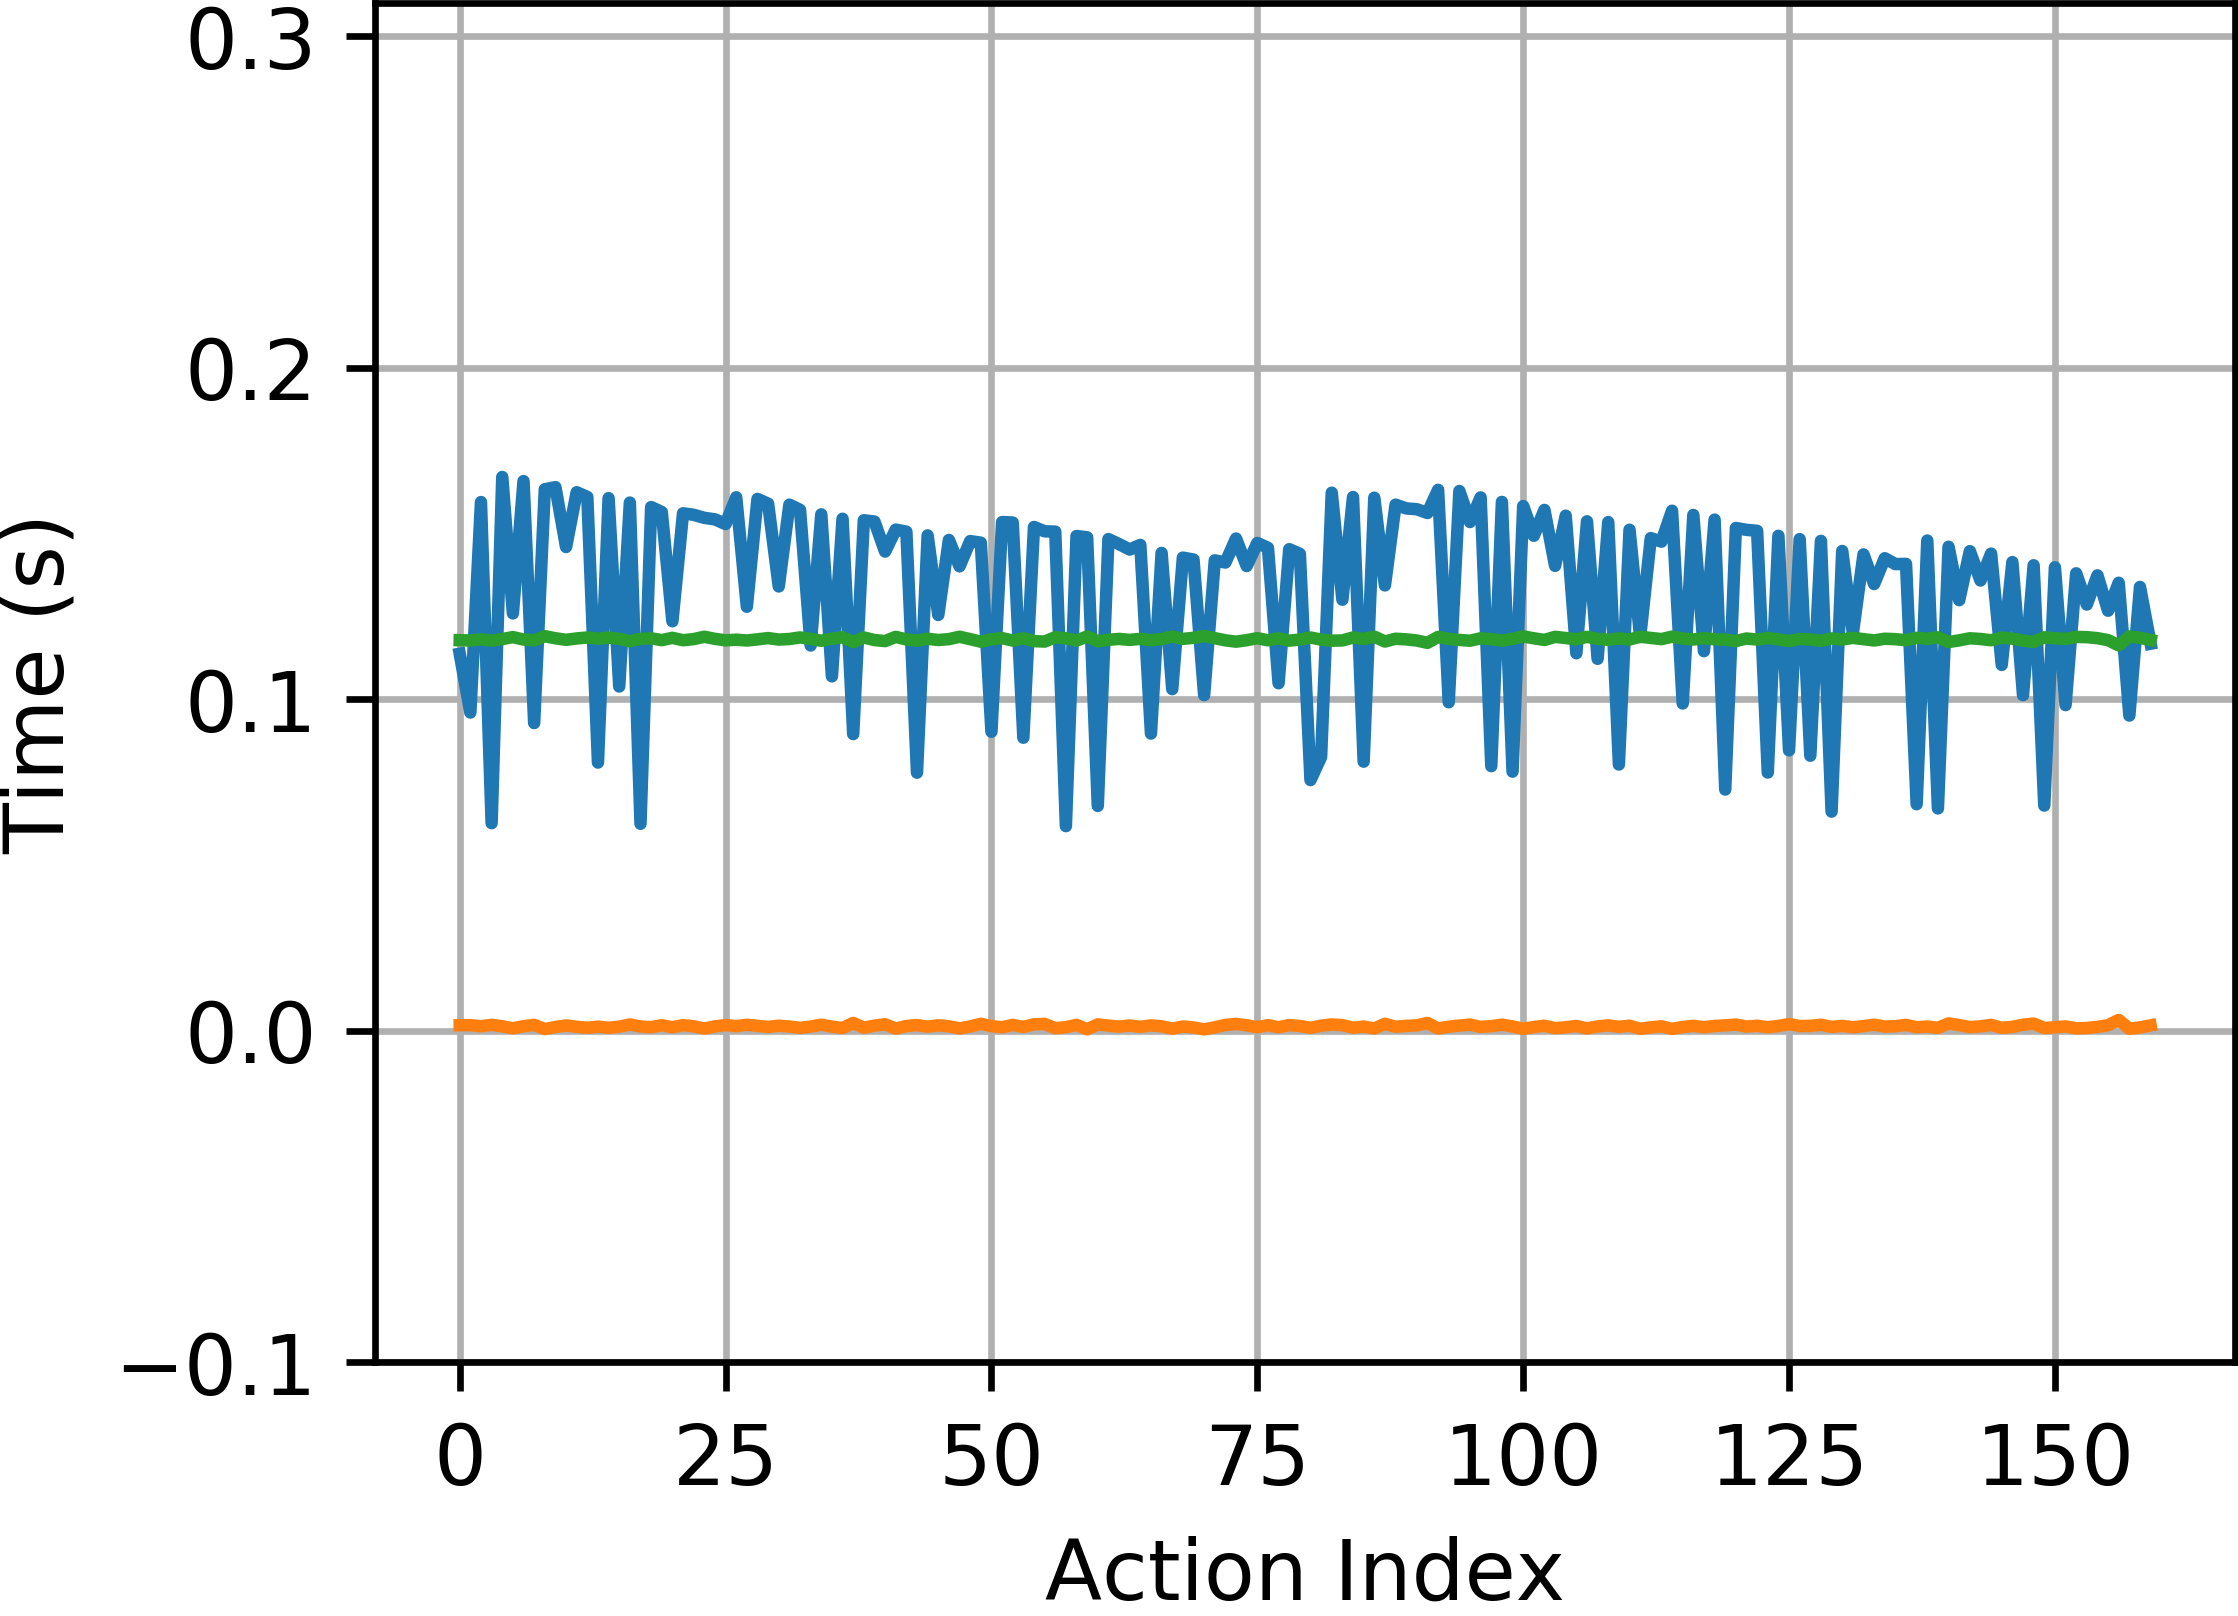
\includegraphics[width=.42\columnwidth]{chapter-gdb-appl/figures/database/WiredBaseline_Time_Components_1.png}\label{gdbappl:fig:database:Time_Wired}}
	\quad
	\subfloat[Wireless Baseline]{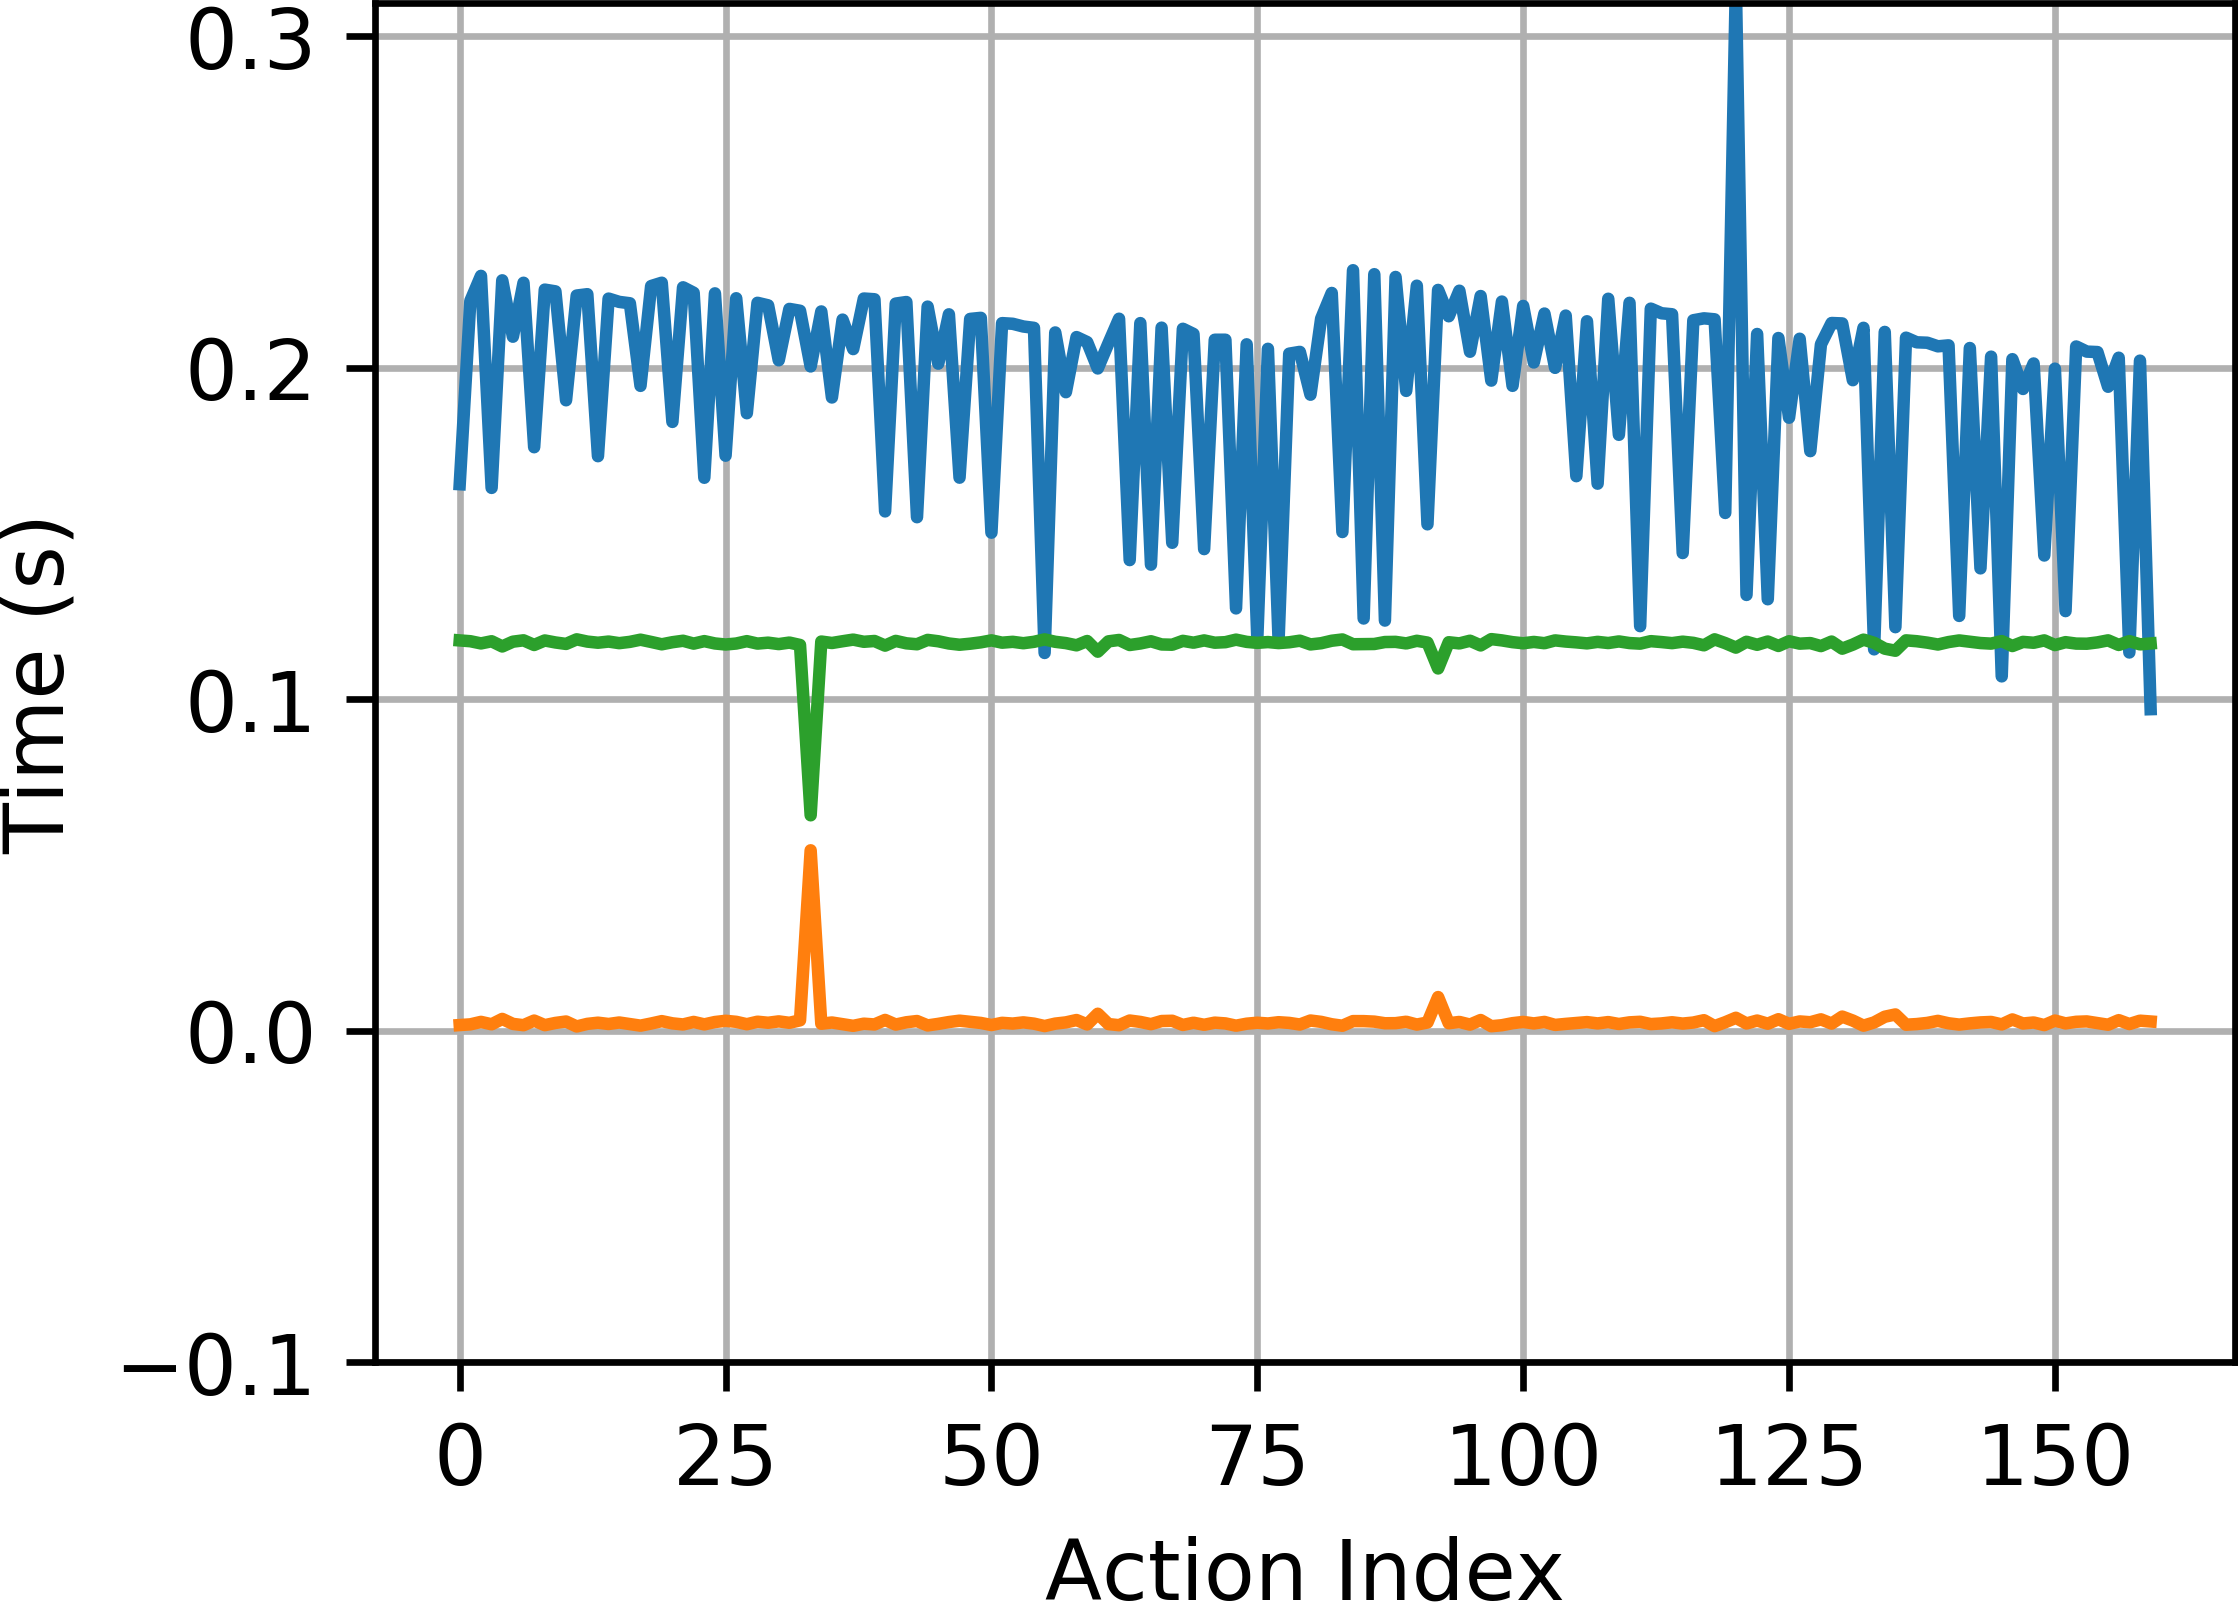
\includegraphics[width=.42\columnwidth]{chapter-gdb-appl/figures/database/WirelessBaseline_Time_Components_1.png} \label{gdbappl:fig:database:Time_Wireless}}\\
	\subfloat[With 2500 pps Traffic (run 1)]{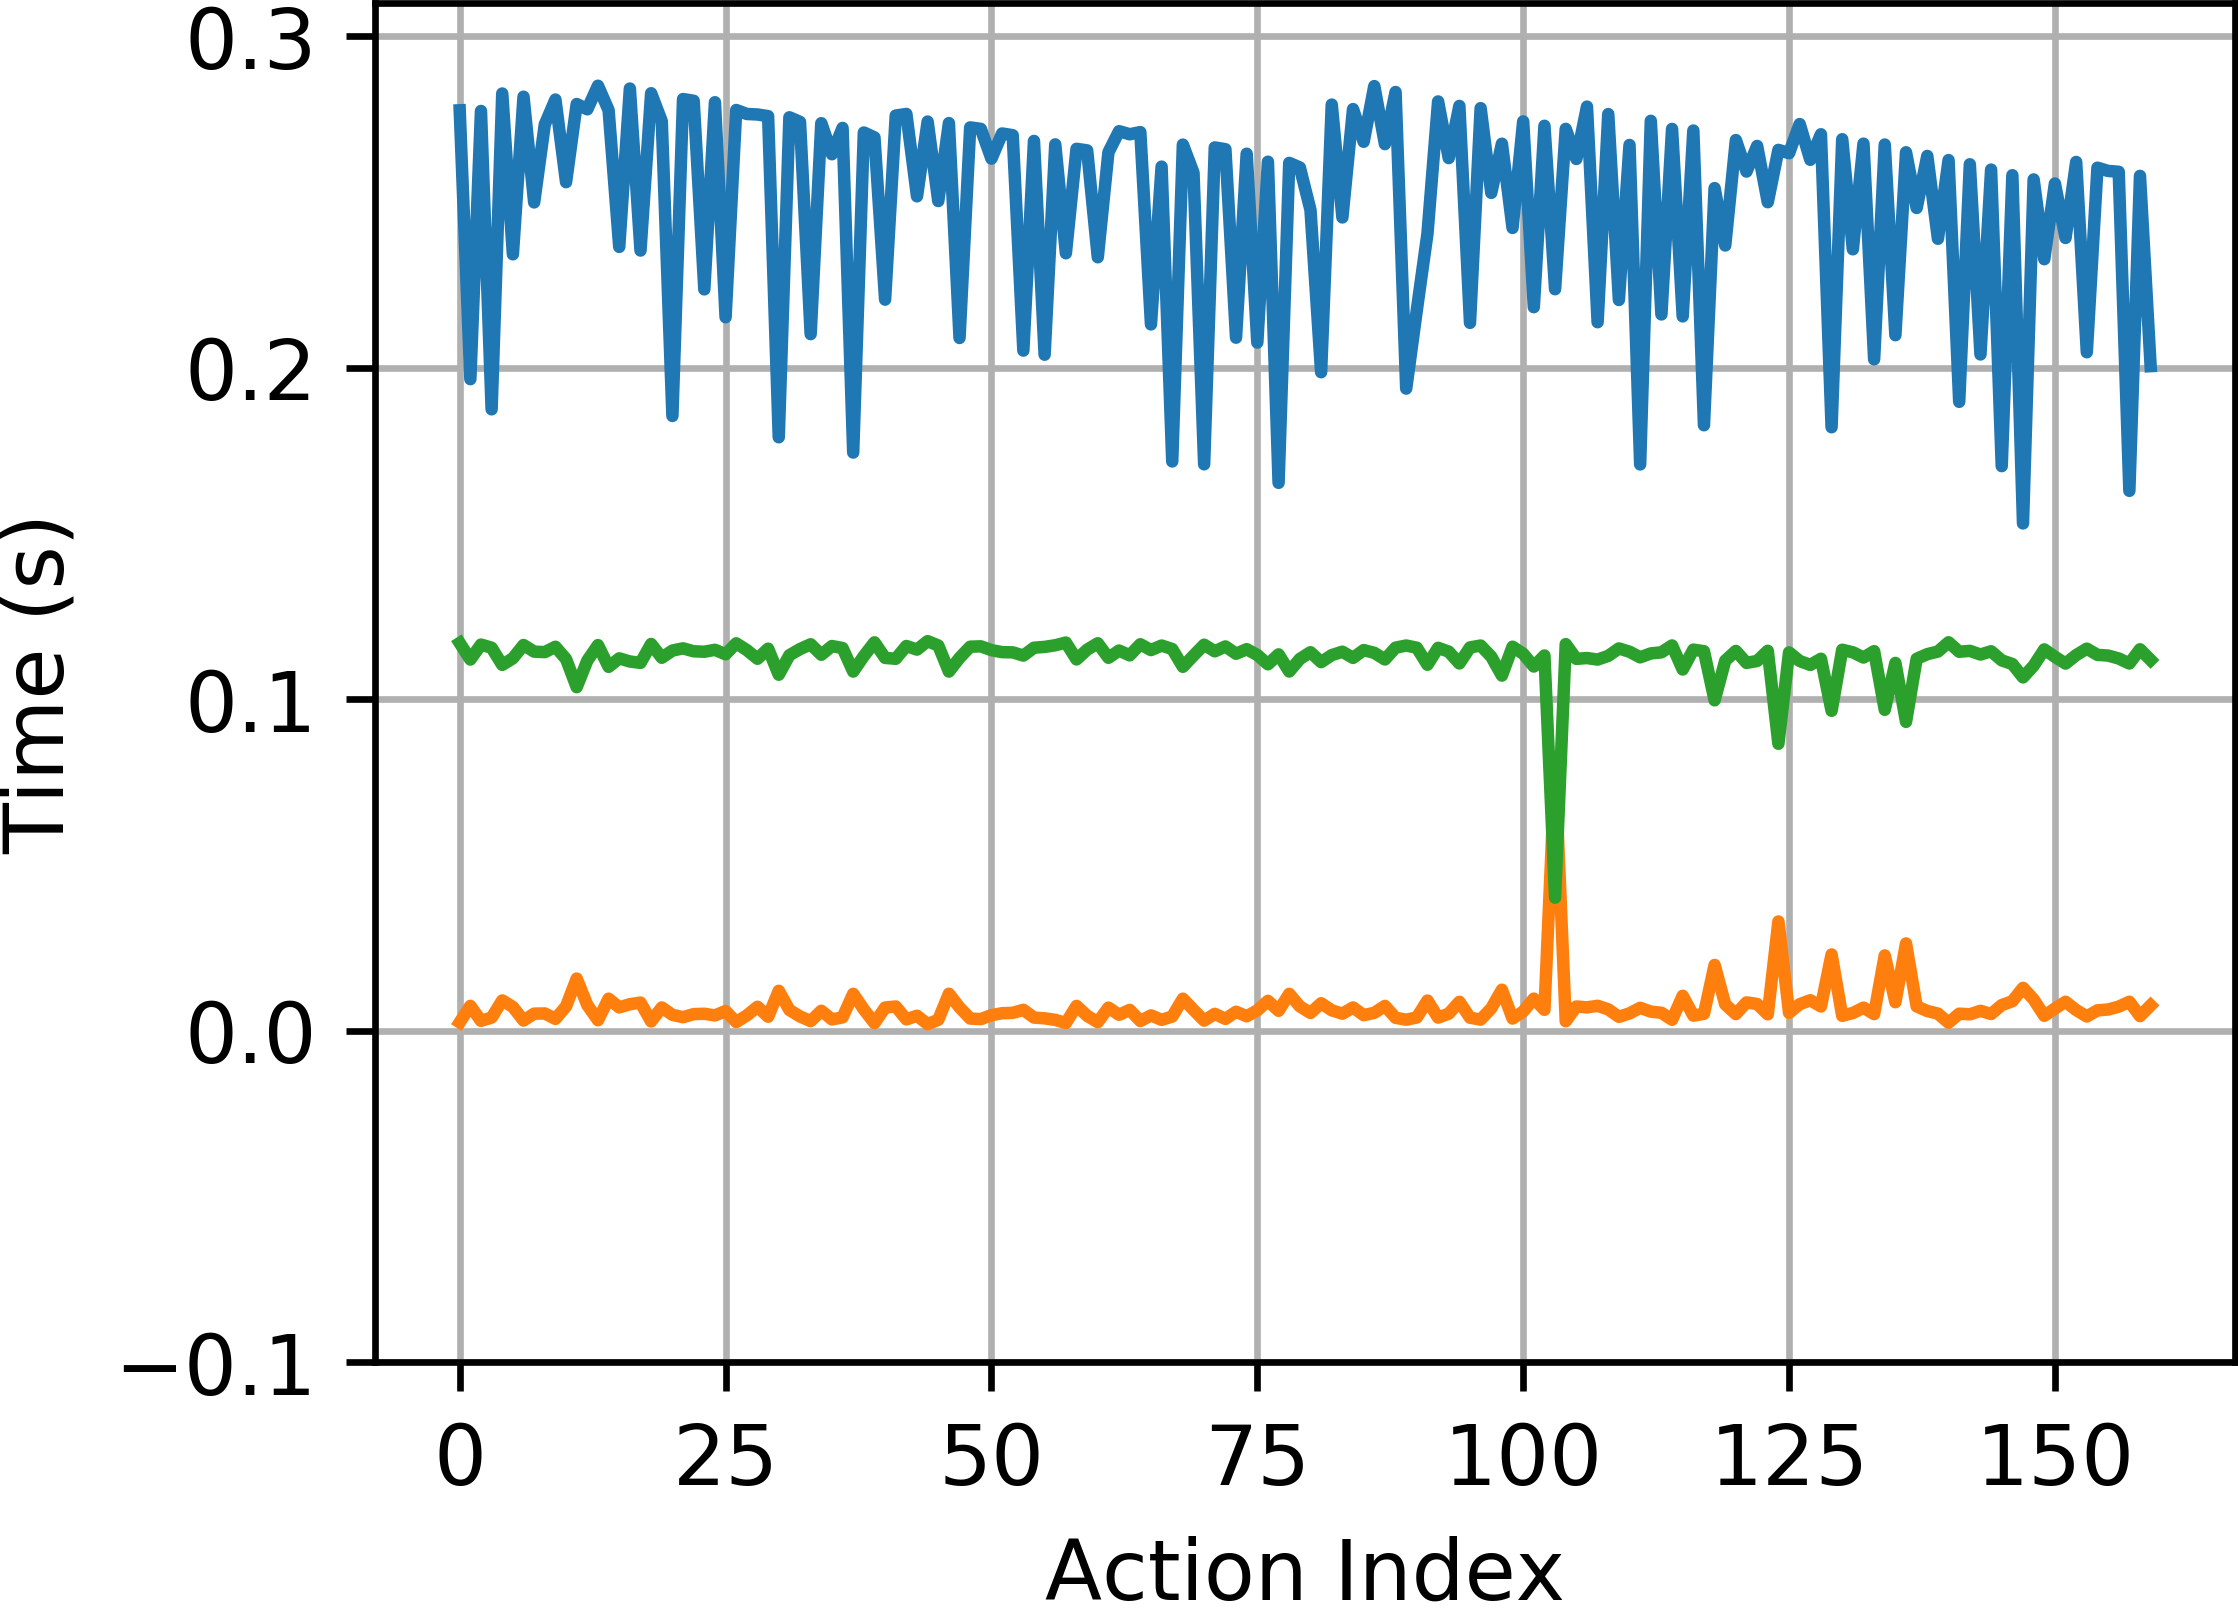
\includegraphics[width=.42\columnwidth]{chapter-gdb-appl/figures/database/2500pps1000Bv1_Time_Components_1.png}
		\label{gdbappl:fig:database:Time_2500v1}}\quad
	\subfloat[With 2500 pps Traffic (run 2)]{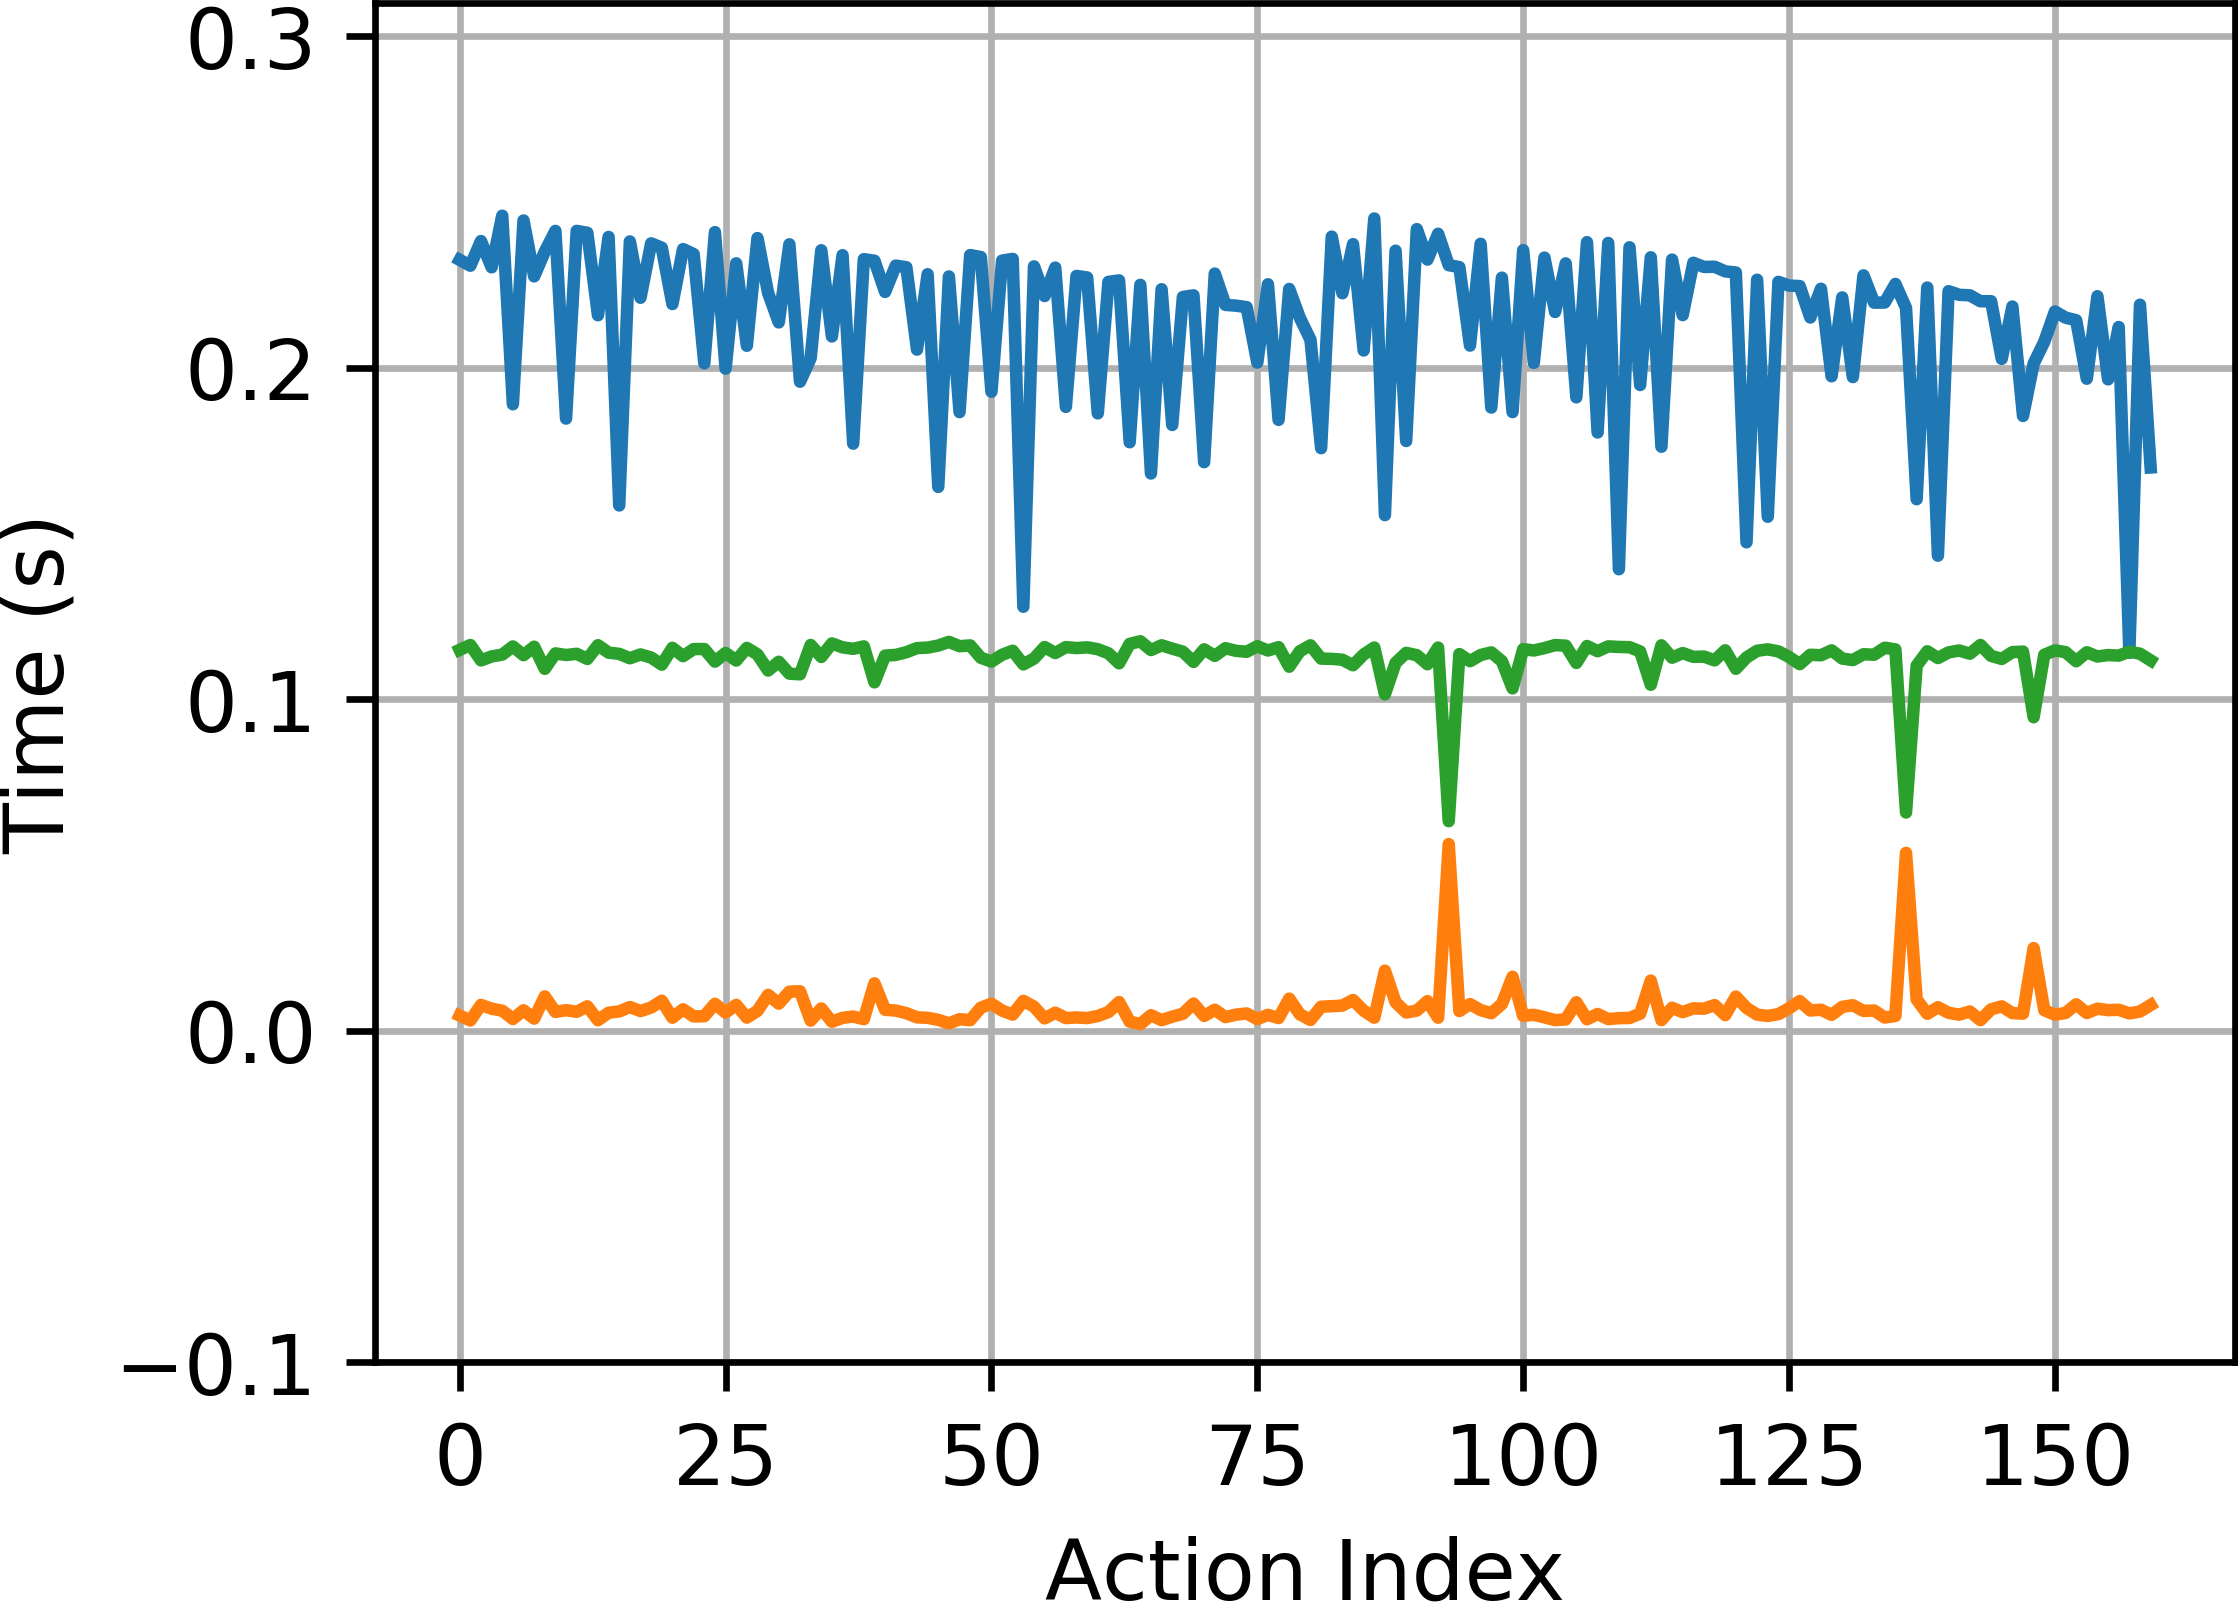
\includegraphics[width=.42\columnwidth]{chapter-gdb-appl/figures/database/2500pps1000Bv2_Time_Components_1.png}
		\label{gdbappl:fig:database:Time_2500v2}}\\
	\subfloat[With 2x1250 pps Traffic]{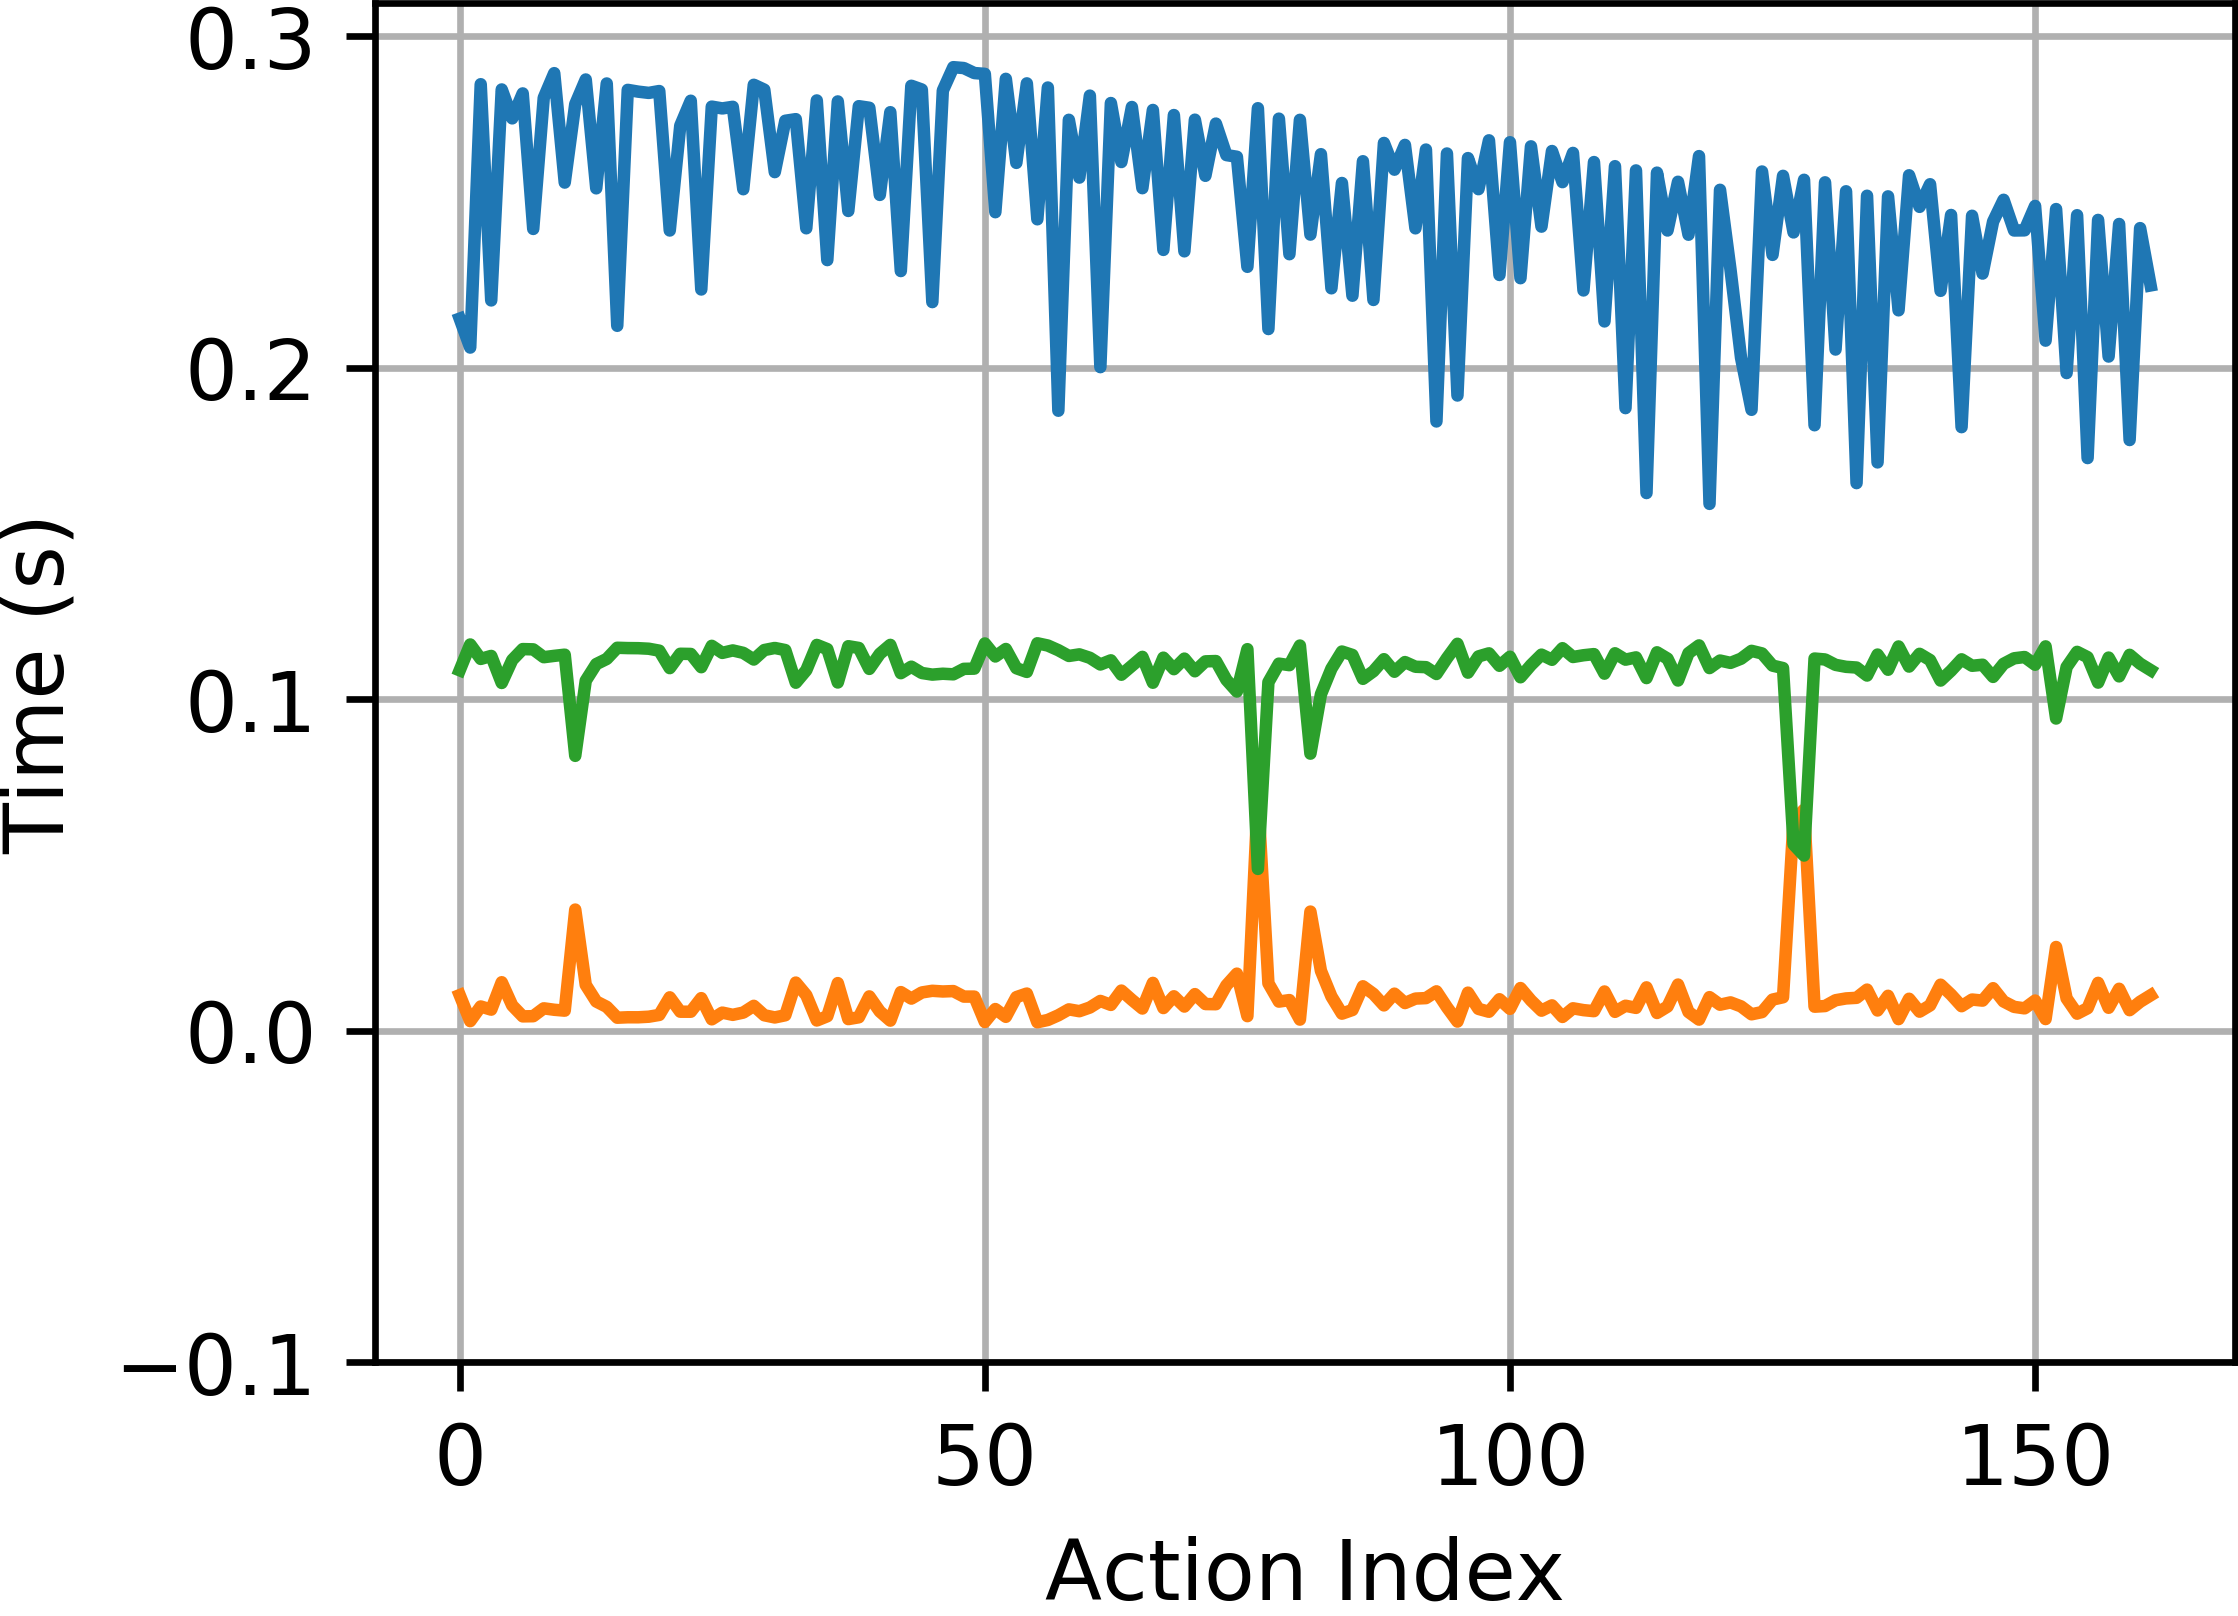
\includegraphics[width=.42\columnwidth]{chapter-gdb-appl/figures/database/2X1250pps1000Bv1_Time_Components_1.png}\label{gdbappl:fig:database:Time_2x1250}}\quad
	{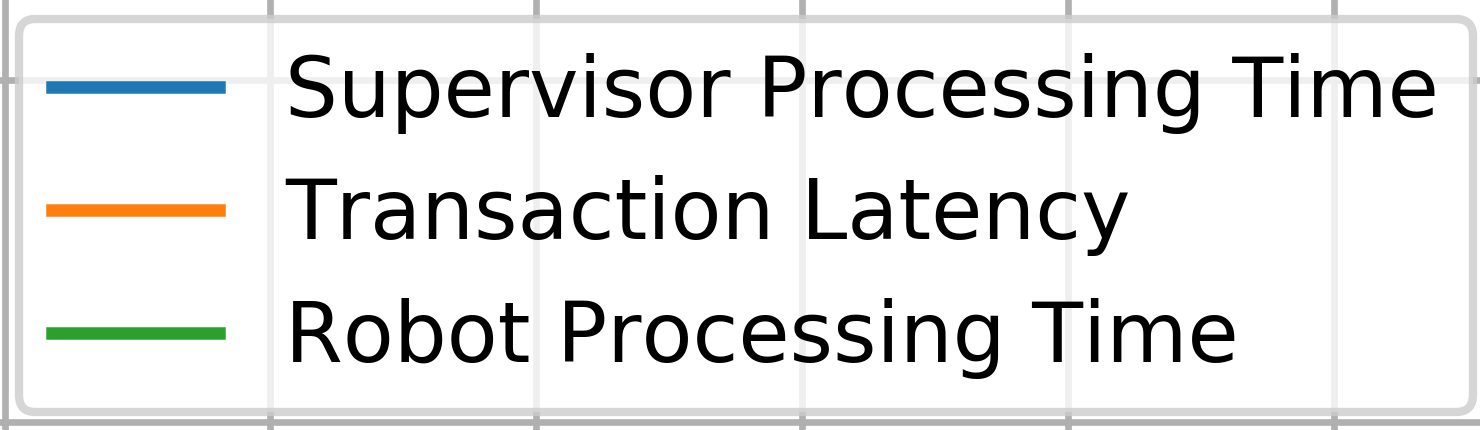
\includegraphics[width=.42\columnwidth]{chapter-gdb-appl/figures/database/Legend.png}}
	\caption{Components of the Physical Action Time for Various Experimental Scenarios.\vspace{-0.2in}}
	\label{gdbappl:fig:database:Time}
\end{figure}

The wired baseline performance is presented in Fig.~\ref{gdbappl:fig:database:Time_Wired} where the transaction latency is almost deterministic. Once wireless network is introduced in Fig.~\ref{gdbappl:fig:database:Time_Wireless}-\ref{gdbappl:fig:database:Time_2x1250}, more randomness in the transaction latency is introduced. Adding the coexisting interference increases the randomness in the transaction latency as shown. We can also notice that when a wireless transaction has a higher latency, the corresponding value of the robot response time is lowered such that the sum of $T_\text{W}+T_\text{Rob}$ has almost a fixed value. This value represents the time needed for one loop through the robot script to scan various registers and initiate the corresponding actions which equals almost 120 ms. In a single loop both the transaction is initiated and the RouteState is updated. Hence in this use case, if the wireless transaction latency value is lower than the robot loop time, the physical action processing time will not be impacted by the wireless transaction latency. On the other hand, most of the randomness in the action processing time results from the supervisor processing time. We also notice that the randomness in the supervisor processing time is not impacted by the wireless channel where multiple runs of the same wireless case with the same interfering traffic have completely different supervisor processing time performance as shown in Fig.~\ref{gdbappl:fig:database:Time_2500v1} and \ref{gdbappl:fig:database:Time_2500v2}.   
     
\subsubsection{Stochastic Distribution of Action Processing Time}
In this subsection, we present the normalized histograms of the transaction latency and the total physical action time in Fig,~\ref{gdbappl:fig:hist1} and \ref{gdbappl:fig:hist2}, respectively. In Fig.~\ref{gdbappl:fig:hist1}, we notice the clear impact of the communication channel and interference on the histogram of the transaction latency where the mean and the variance are clearly impacted by the wireless parameters. On the other hand, the total physical action time is not impacted directly by the communications channel in this use case due to the fact that the robot processing loop compensate of any transaction latency below the loop time of 120 ms. 

\begin{figure}[!htbp]
	\centering
	\subfloat[Wired Baseline]{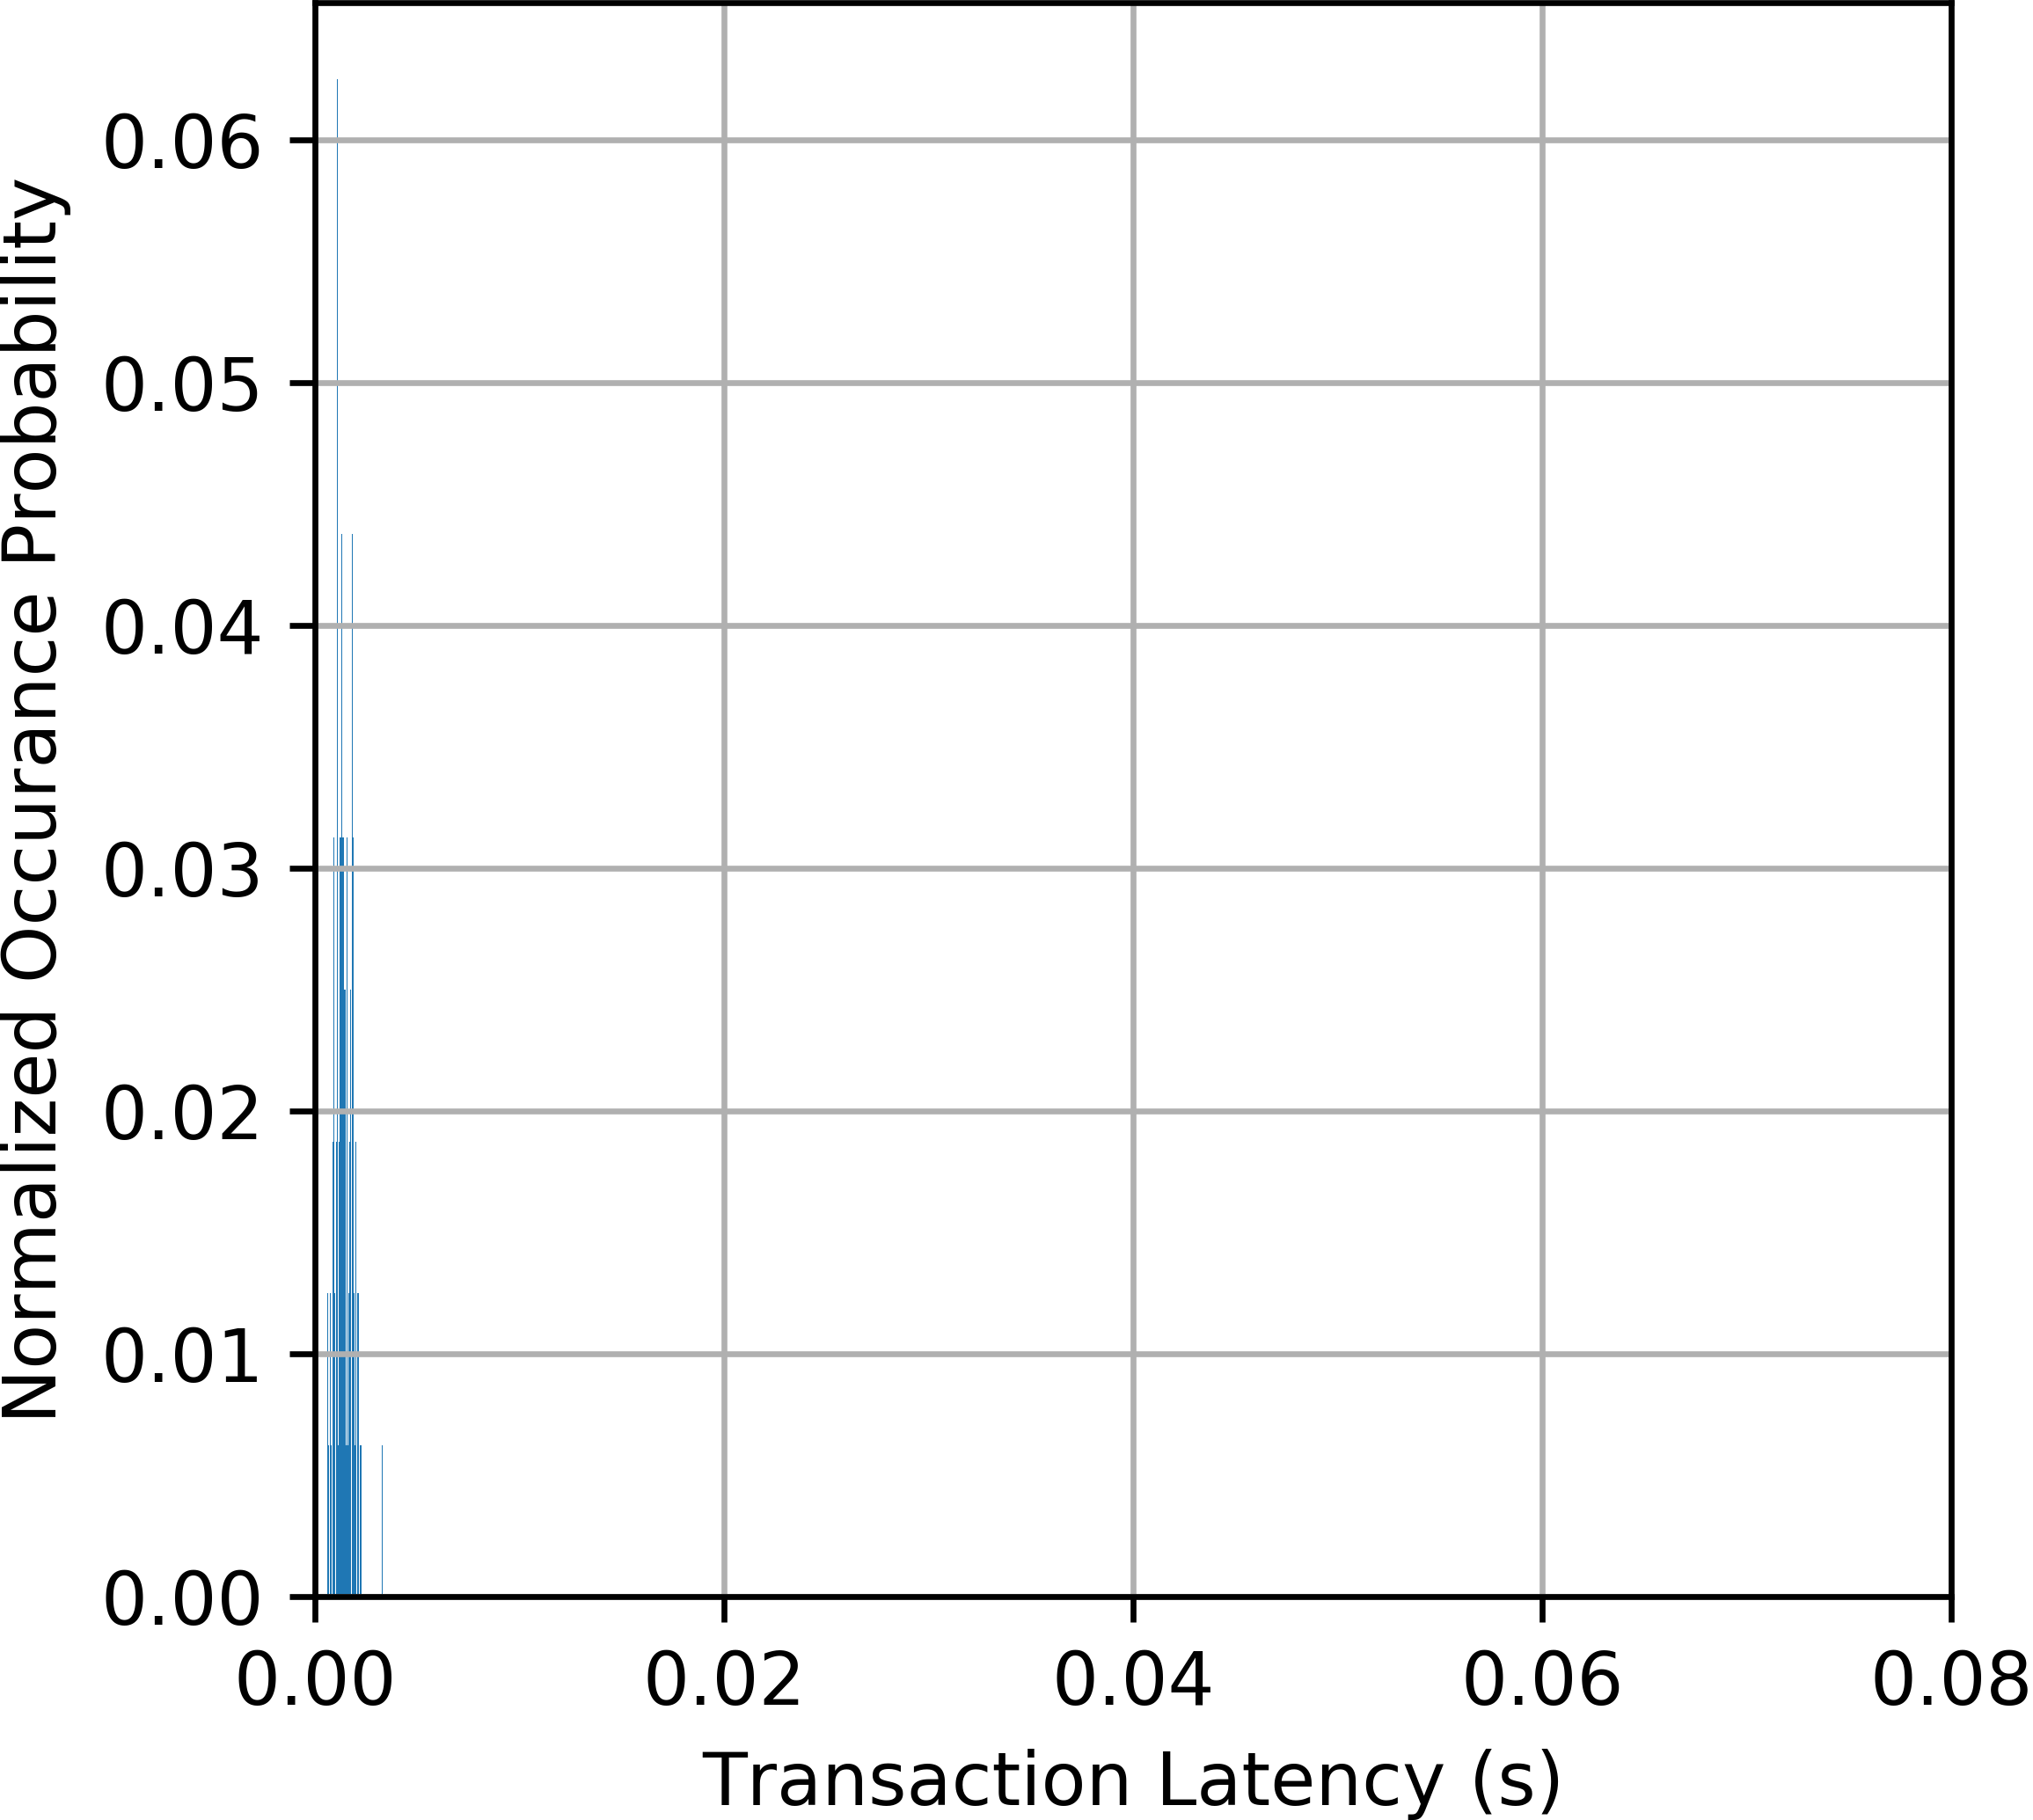
\includegraphics[width=.42\columnwidth]{chapter-gdb-appl/figures/database/WiredBaseline_Hist_1.png}}\quad
	\subfloat[Wireless Baseline]{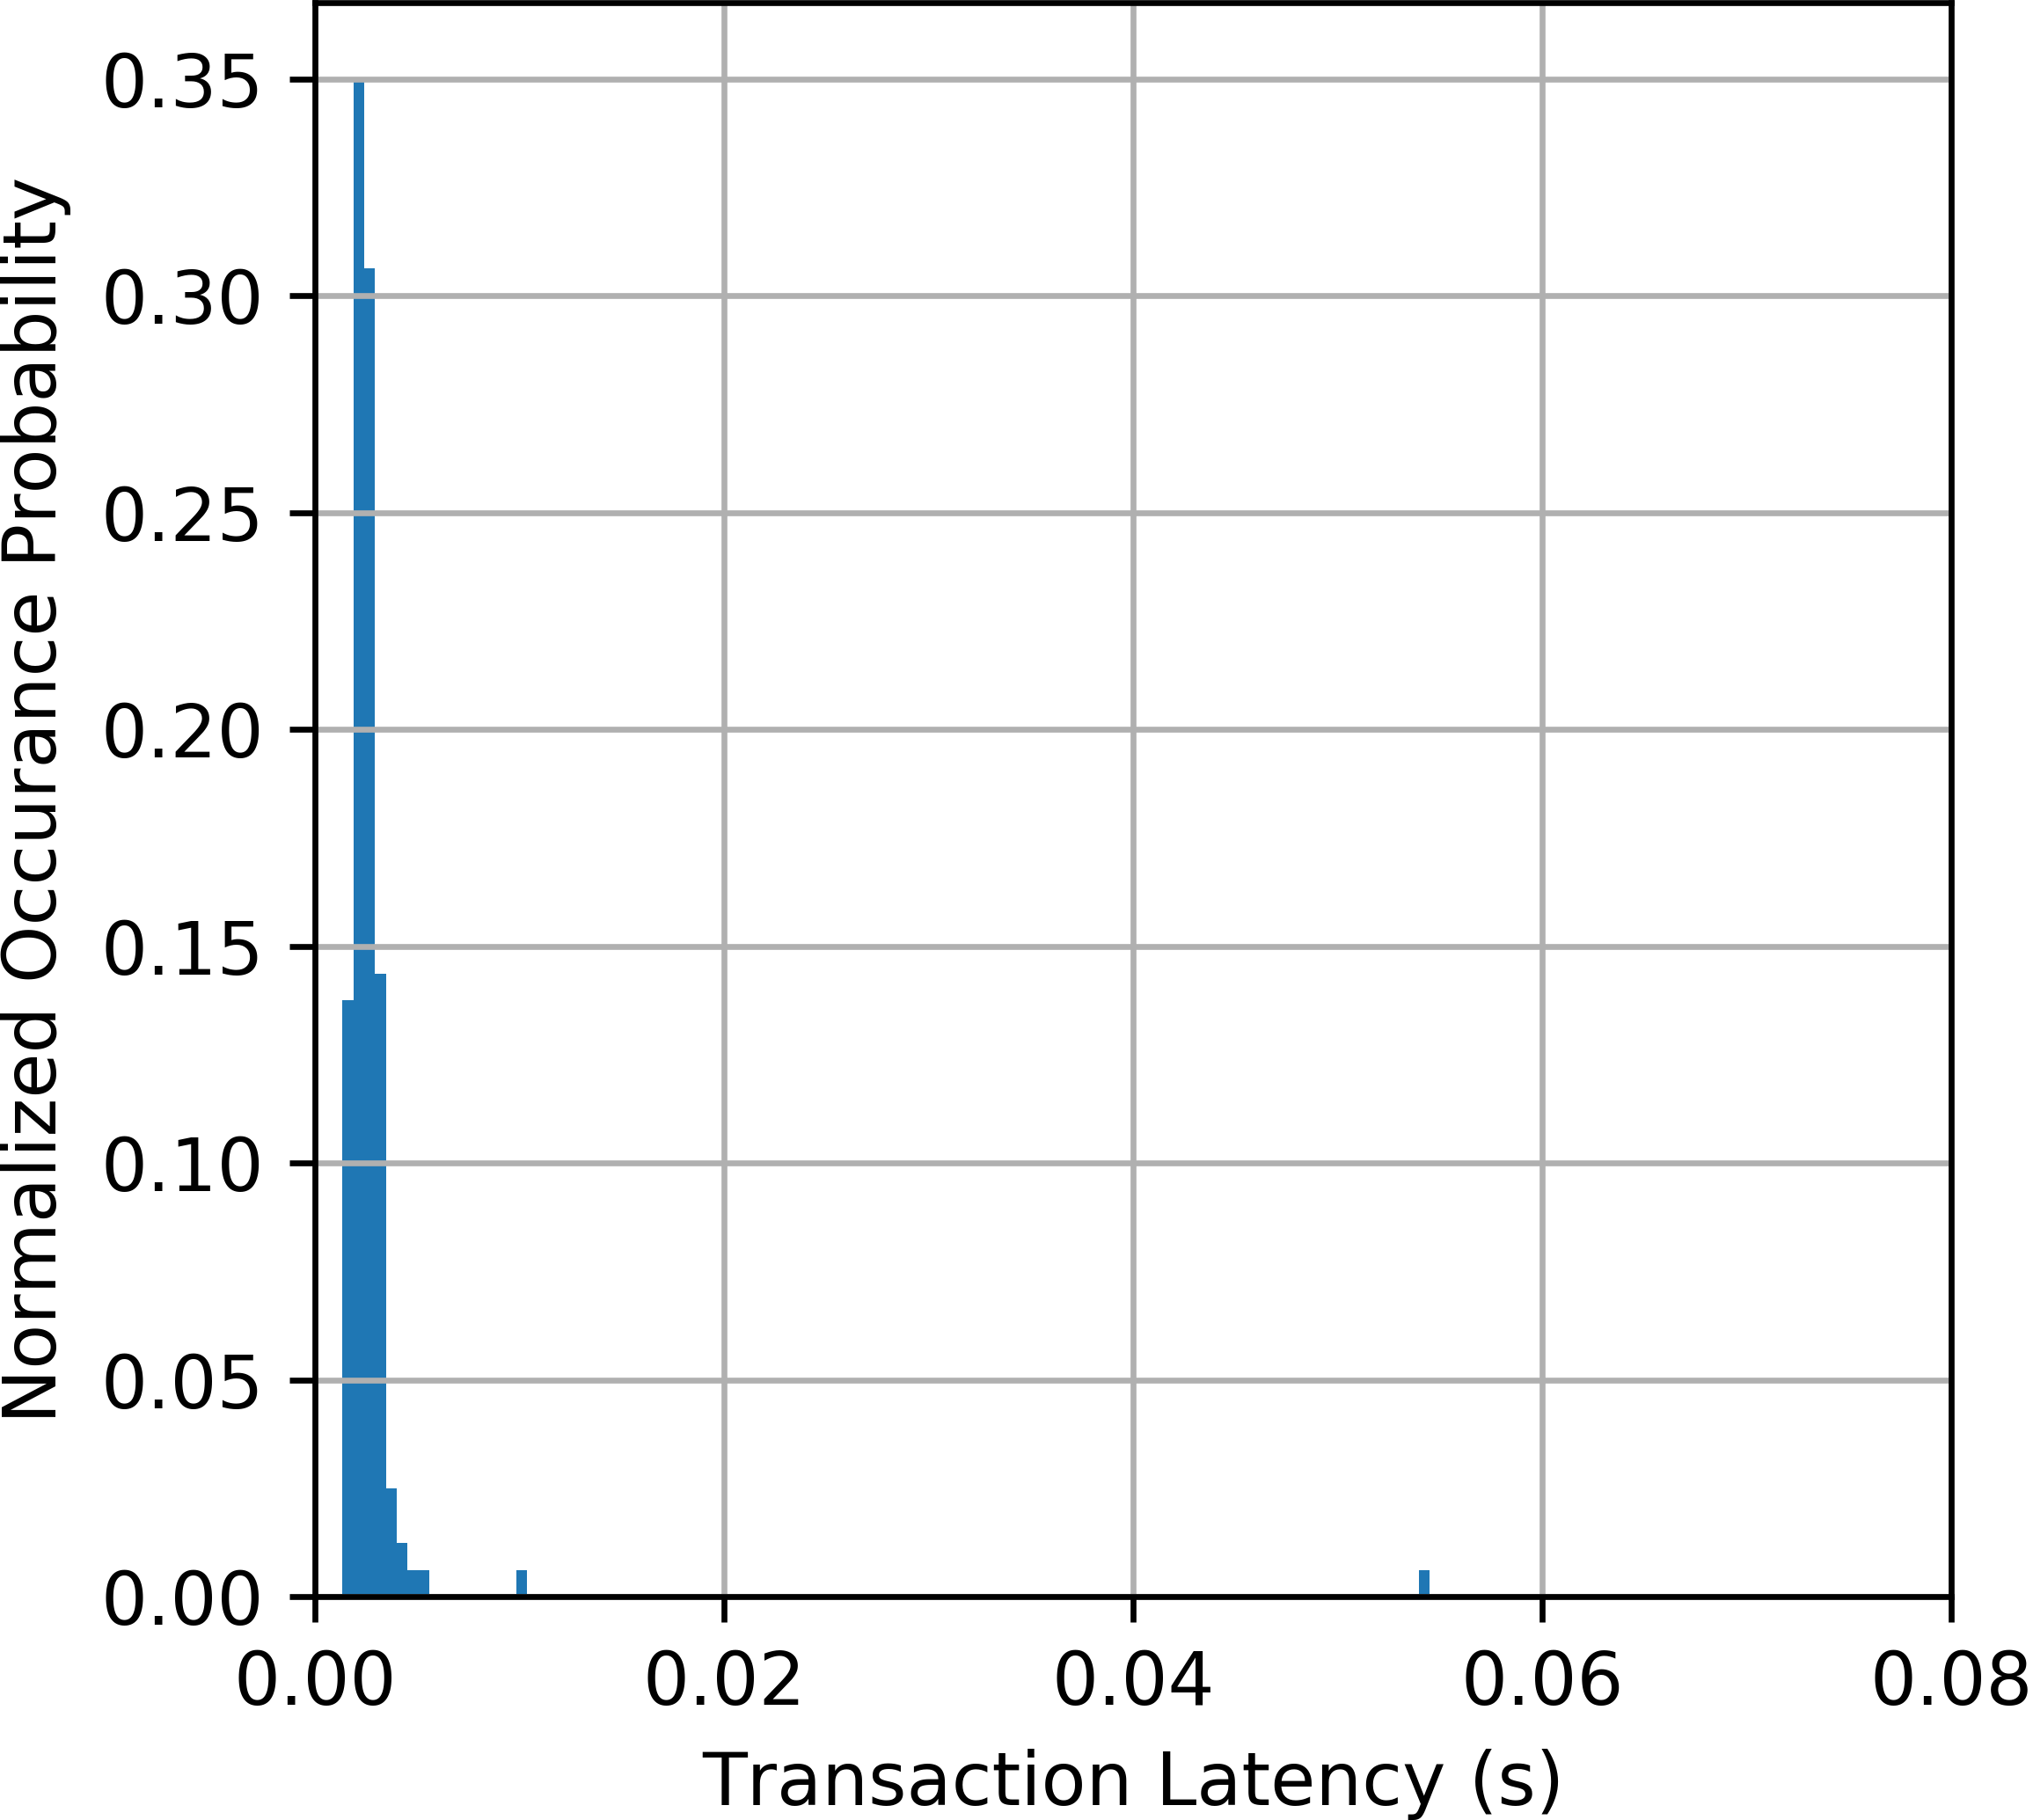
\includegraphics[width=.42\columnwidth]{chapter-gdb-appl/figures/database/WirelessBaseline_Hist_1.png}}\\
	\subfloat[With 2500 pps Traffic]{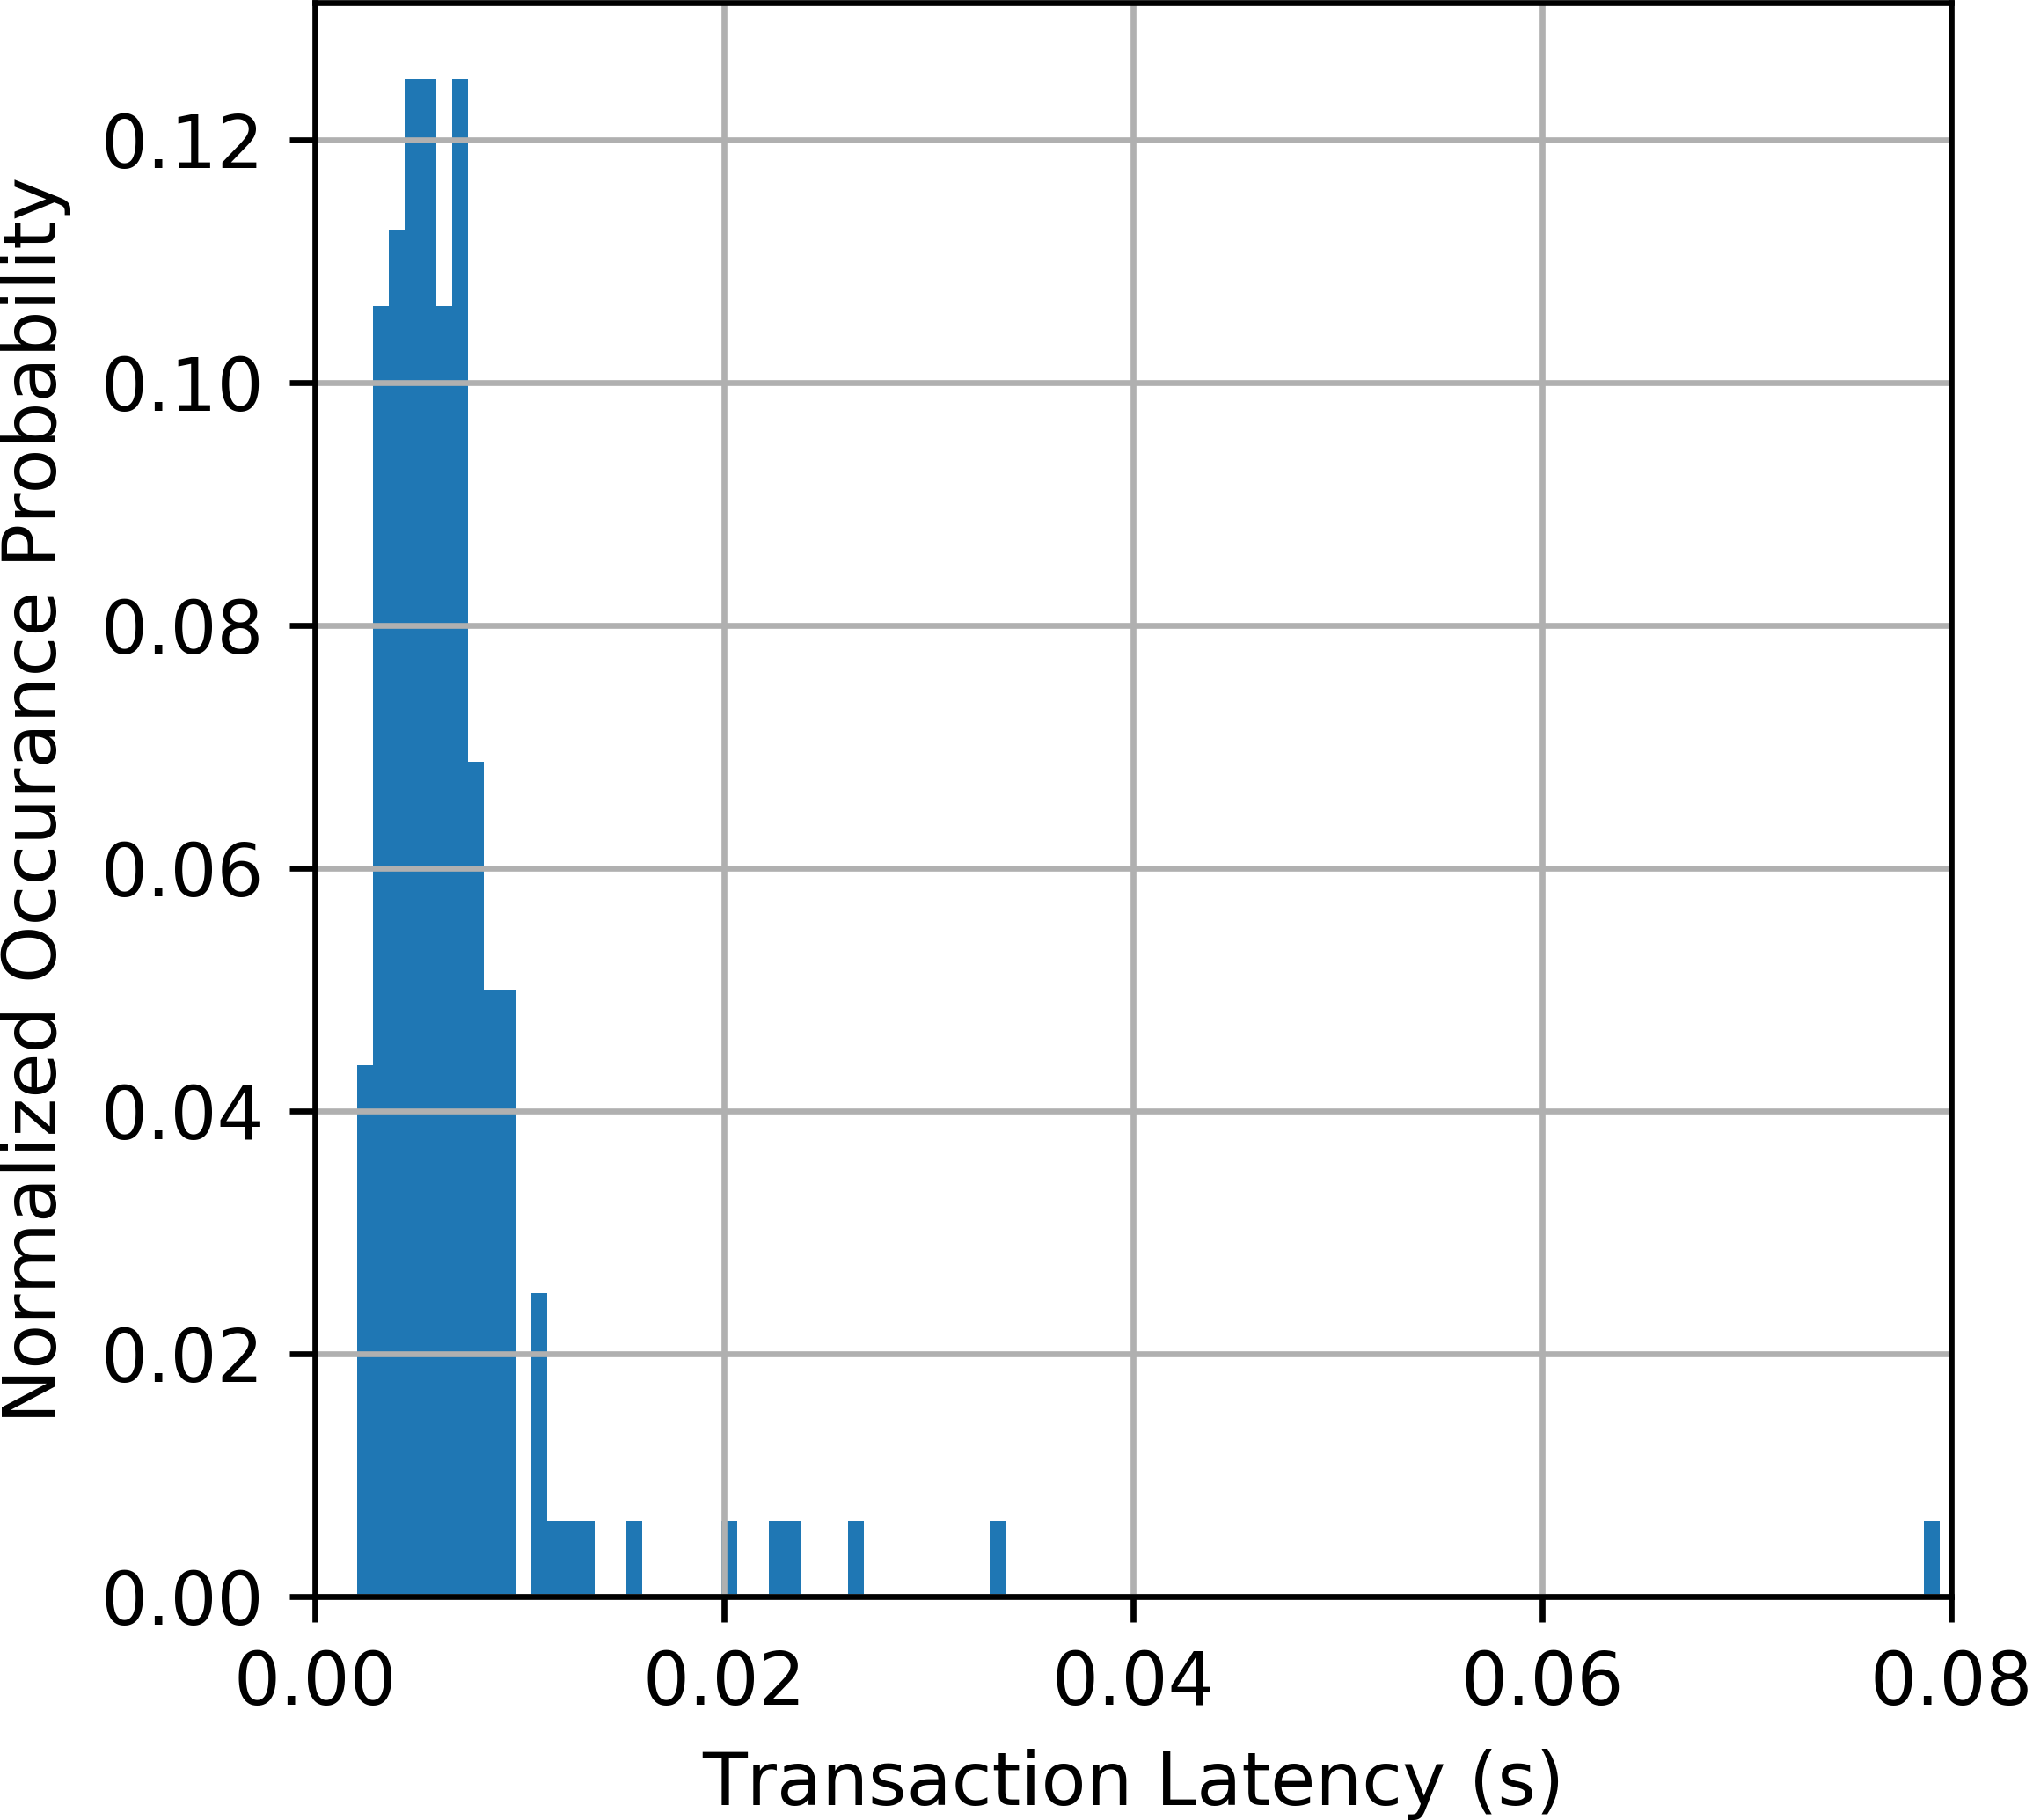
\includegraphics[width=.42\columnwidth]{chapter-gdb-appl/figures/database/2500pps1000Bv1_Hist_1.png}
		\label{With 2500 packets/s Traffic}}\quad
	\subfloat[With 2x1250 pps Traffic]{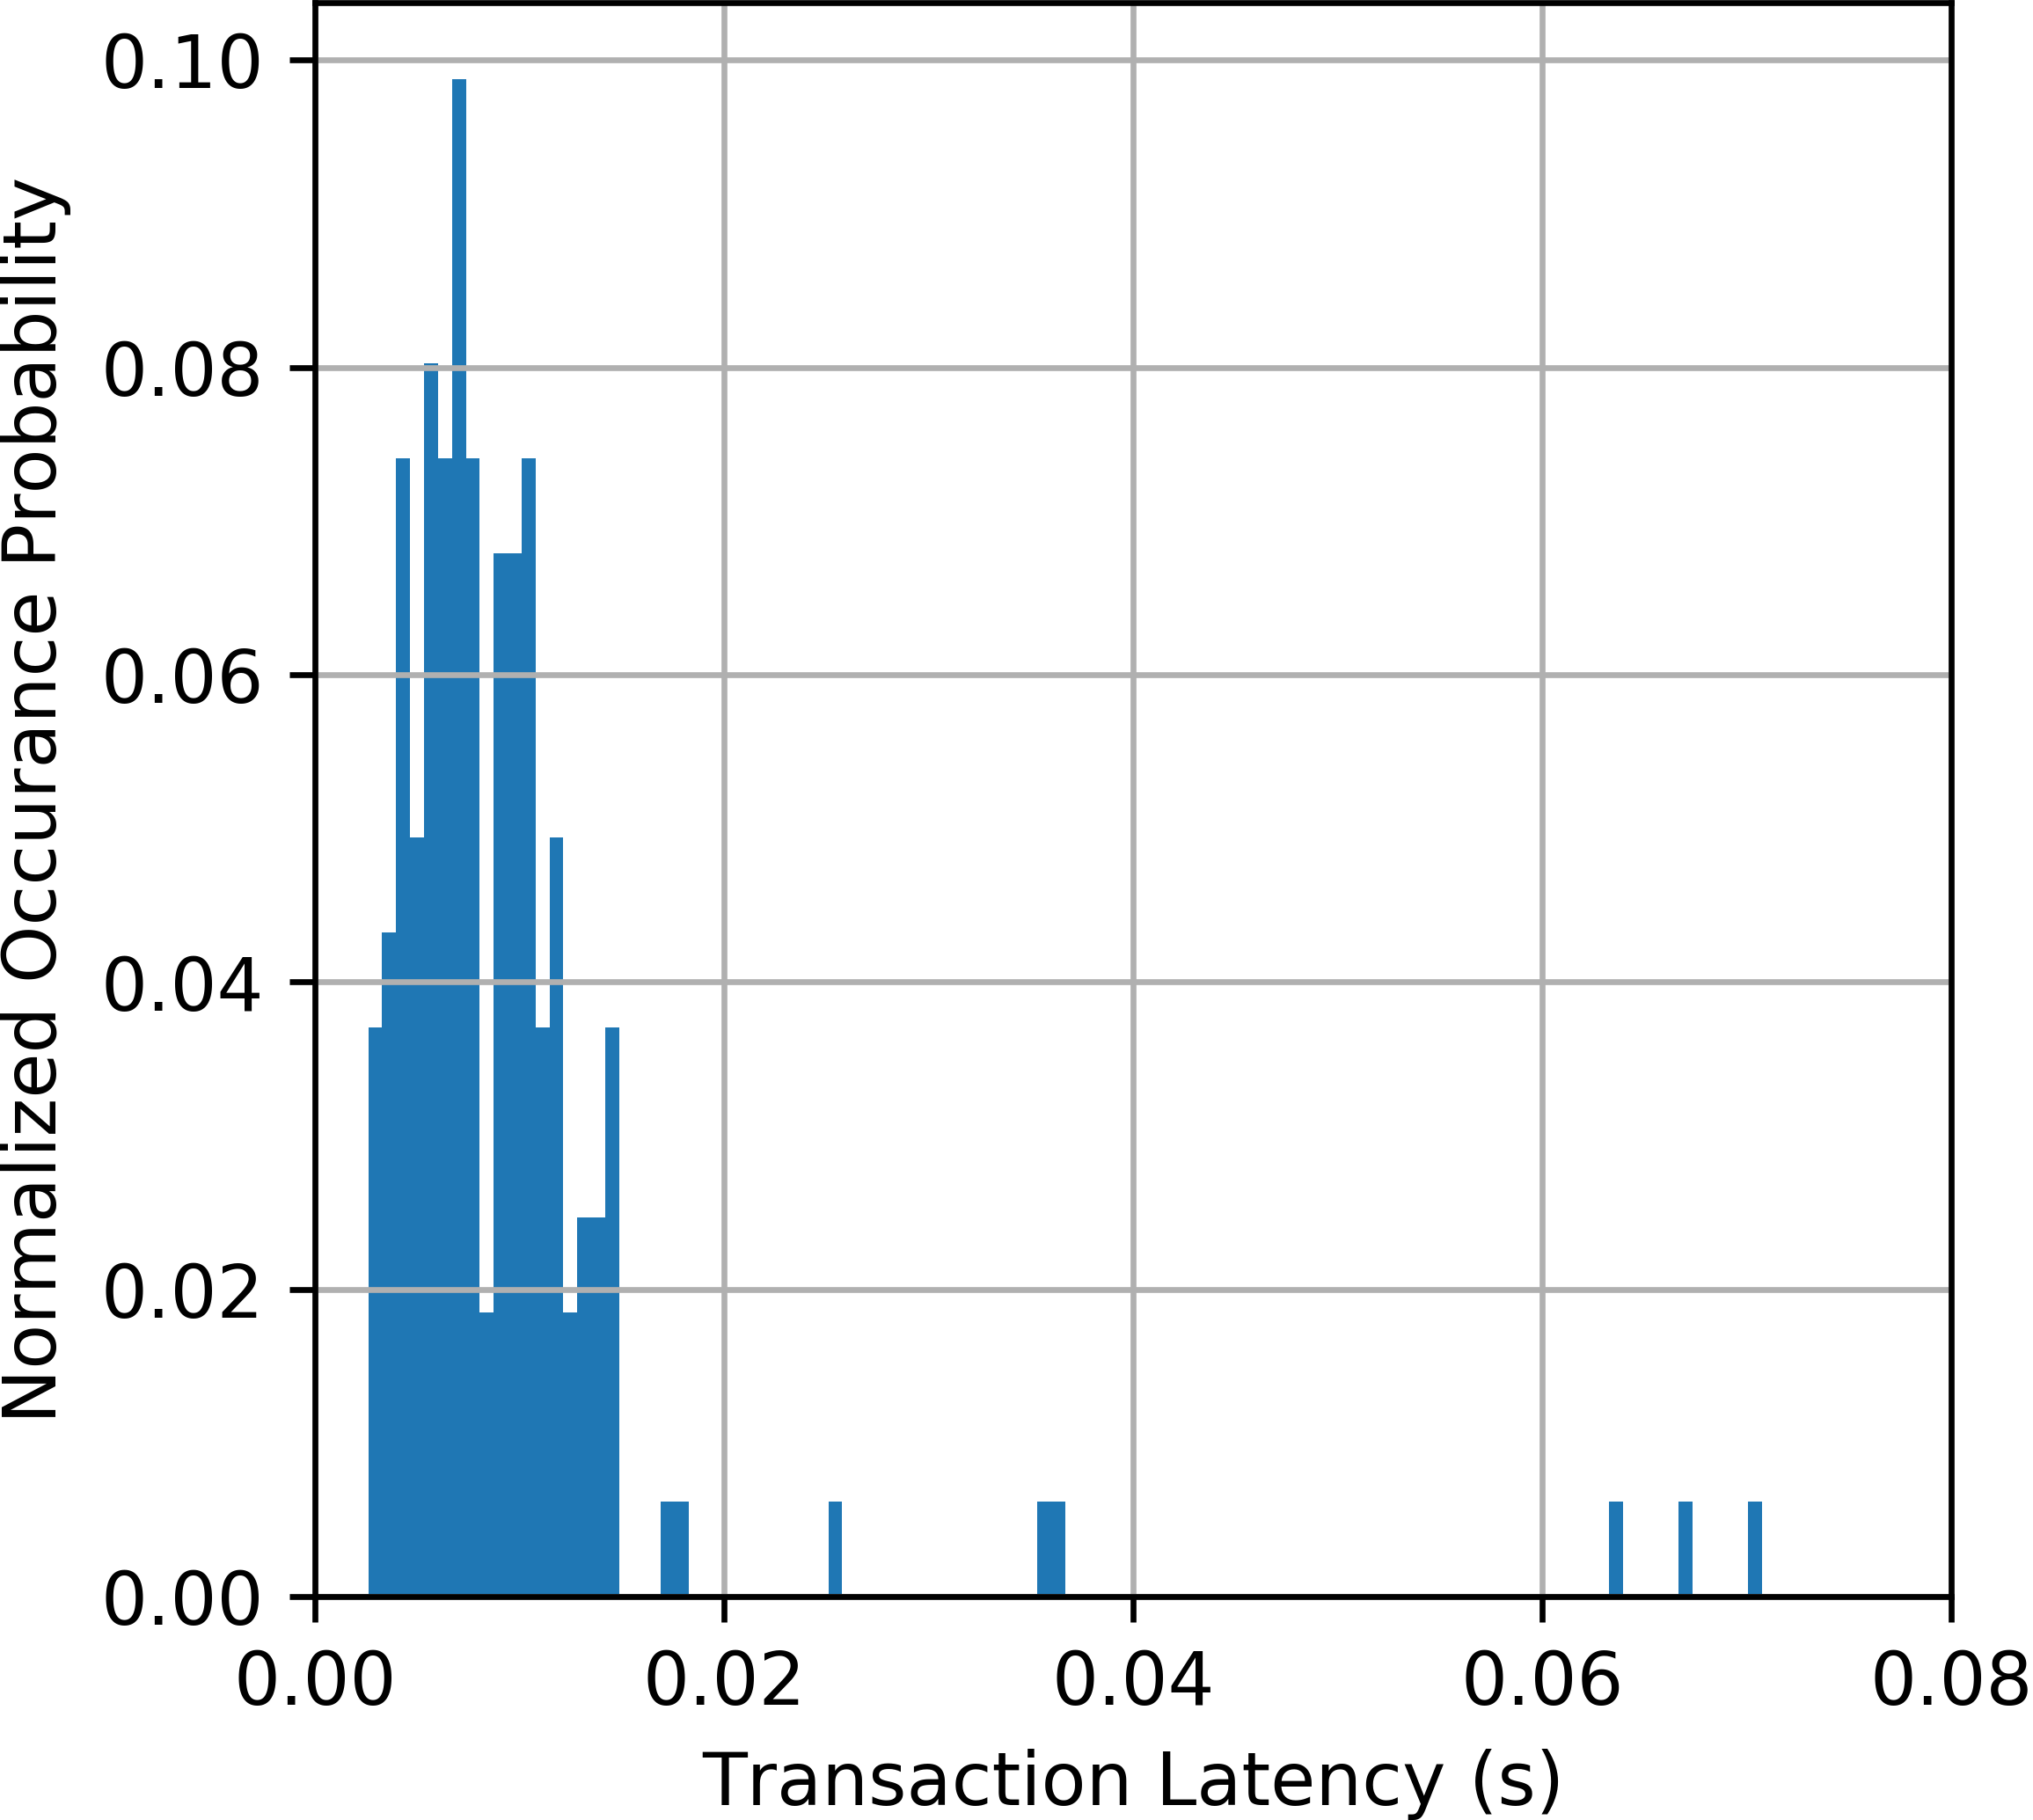
\includegraphics[width=.42\columnwidth]{chapter-gdb-appl/figures/database/2X1250pps1000Bv1_Hist_1.png}}
	\caption{Histograms of Transaction Latency for Various Experimental Scenarios.}
	\label{gdbappl:fig:hist1}
\end{figure}

\begin{figure}[!htbp]
	\centering
	\subfloat[Wired Baseline]{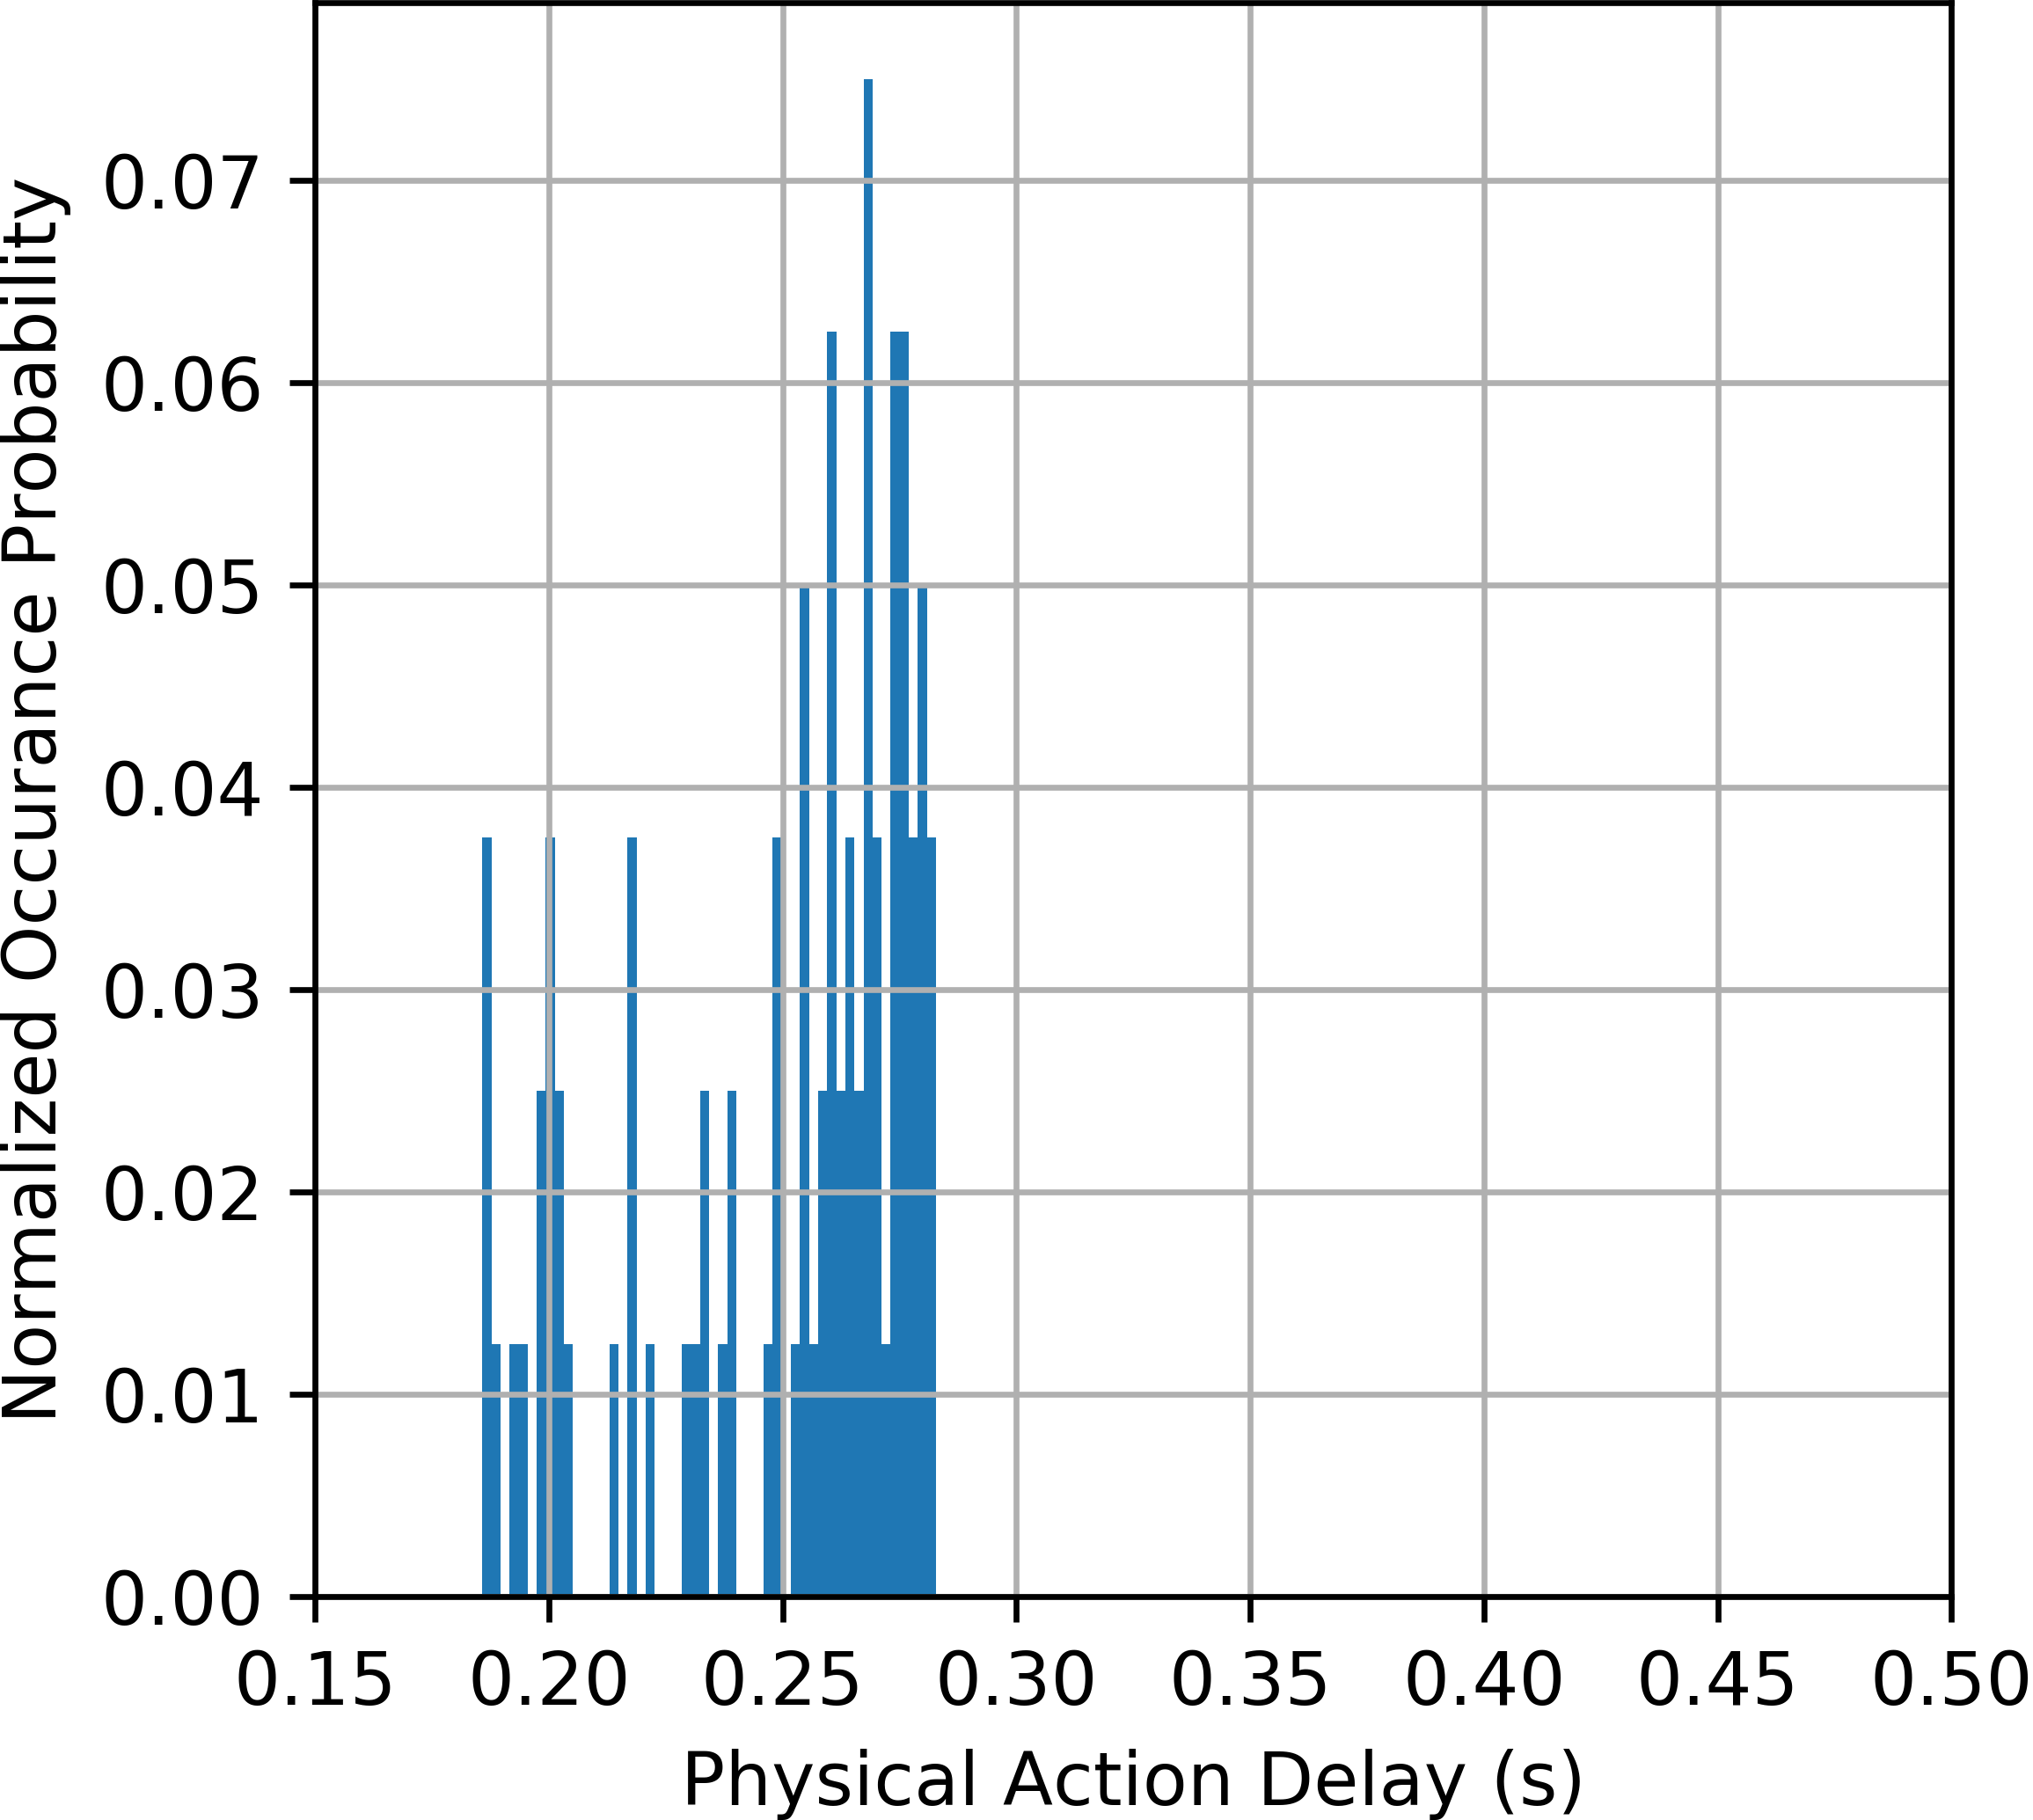
\includegraphics[width=.42\columnwidth]{chapter-gdb-appl/figures/database/WiredBaseline_PhyHist_1.png}}\quad
	\subfloat[Wireless Baseline]{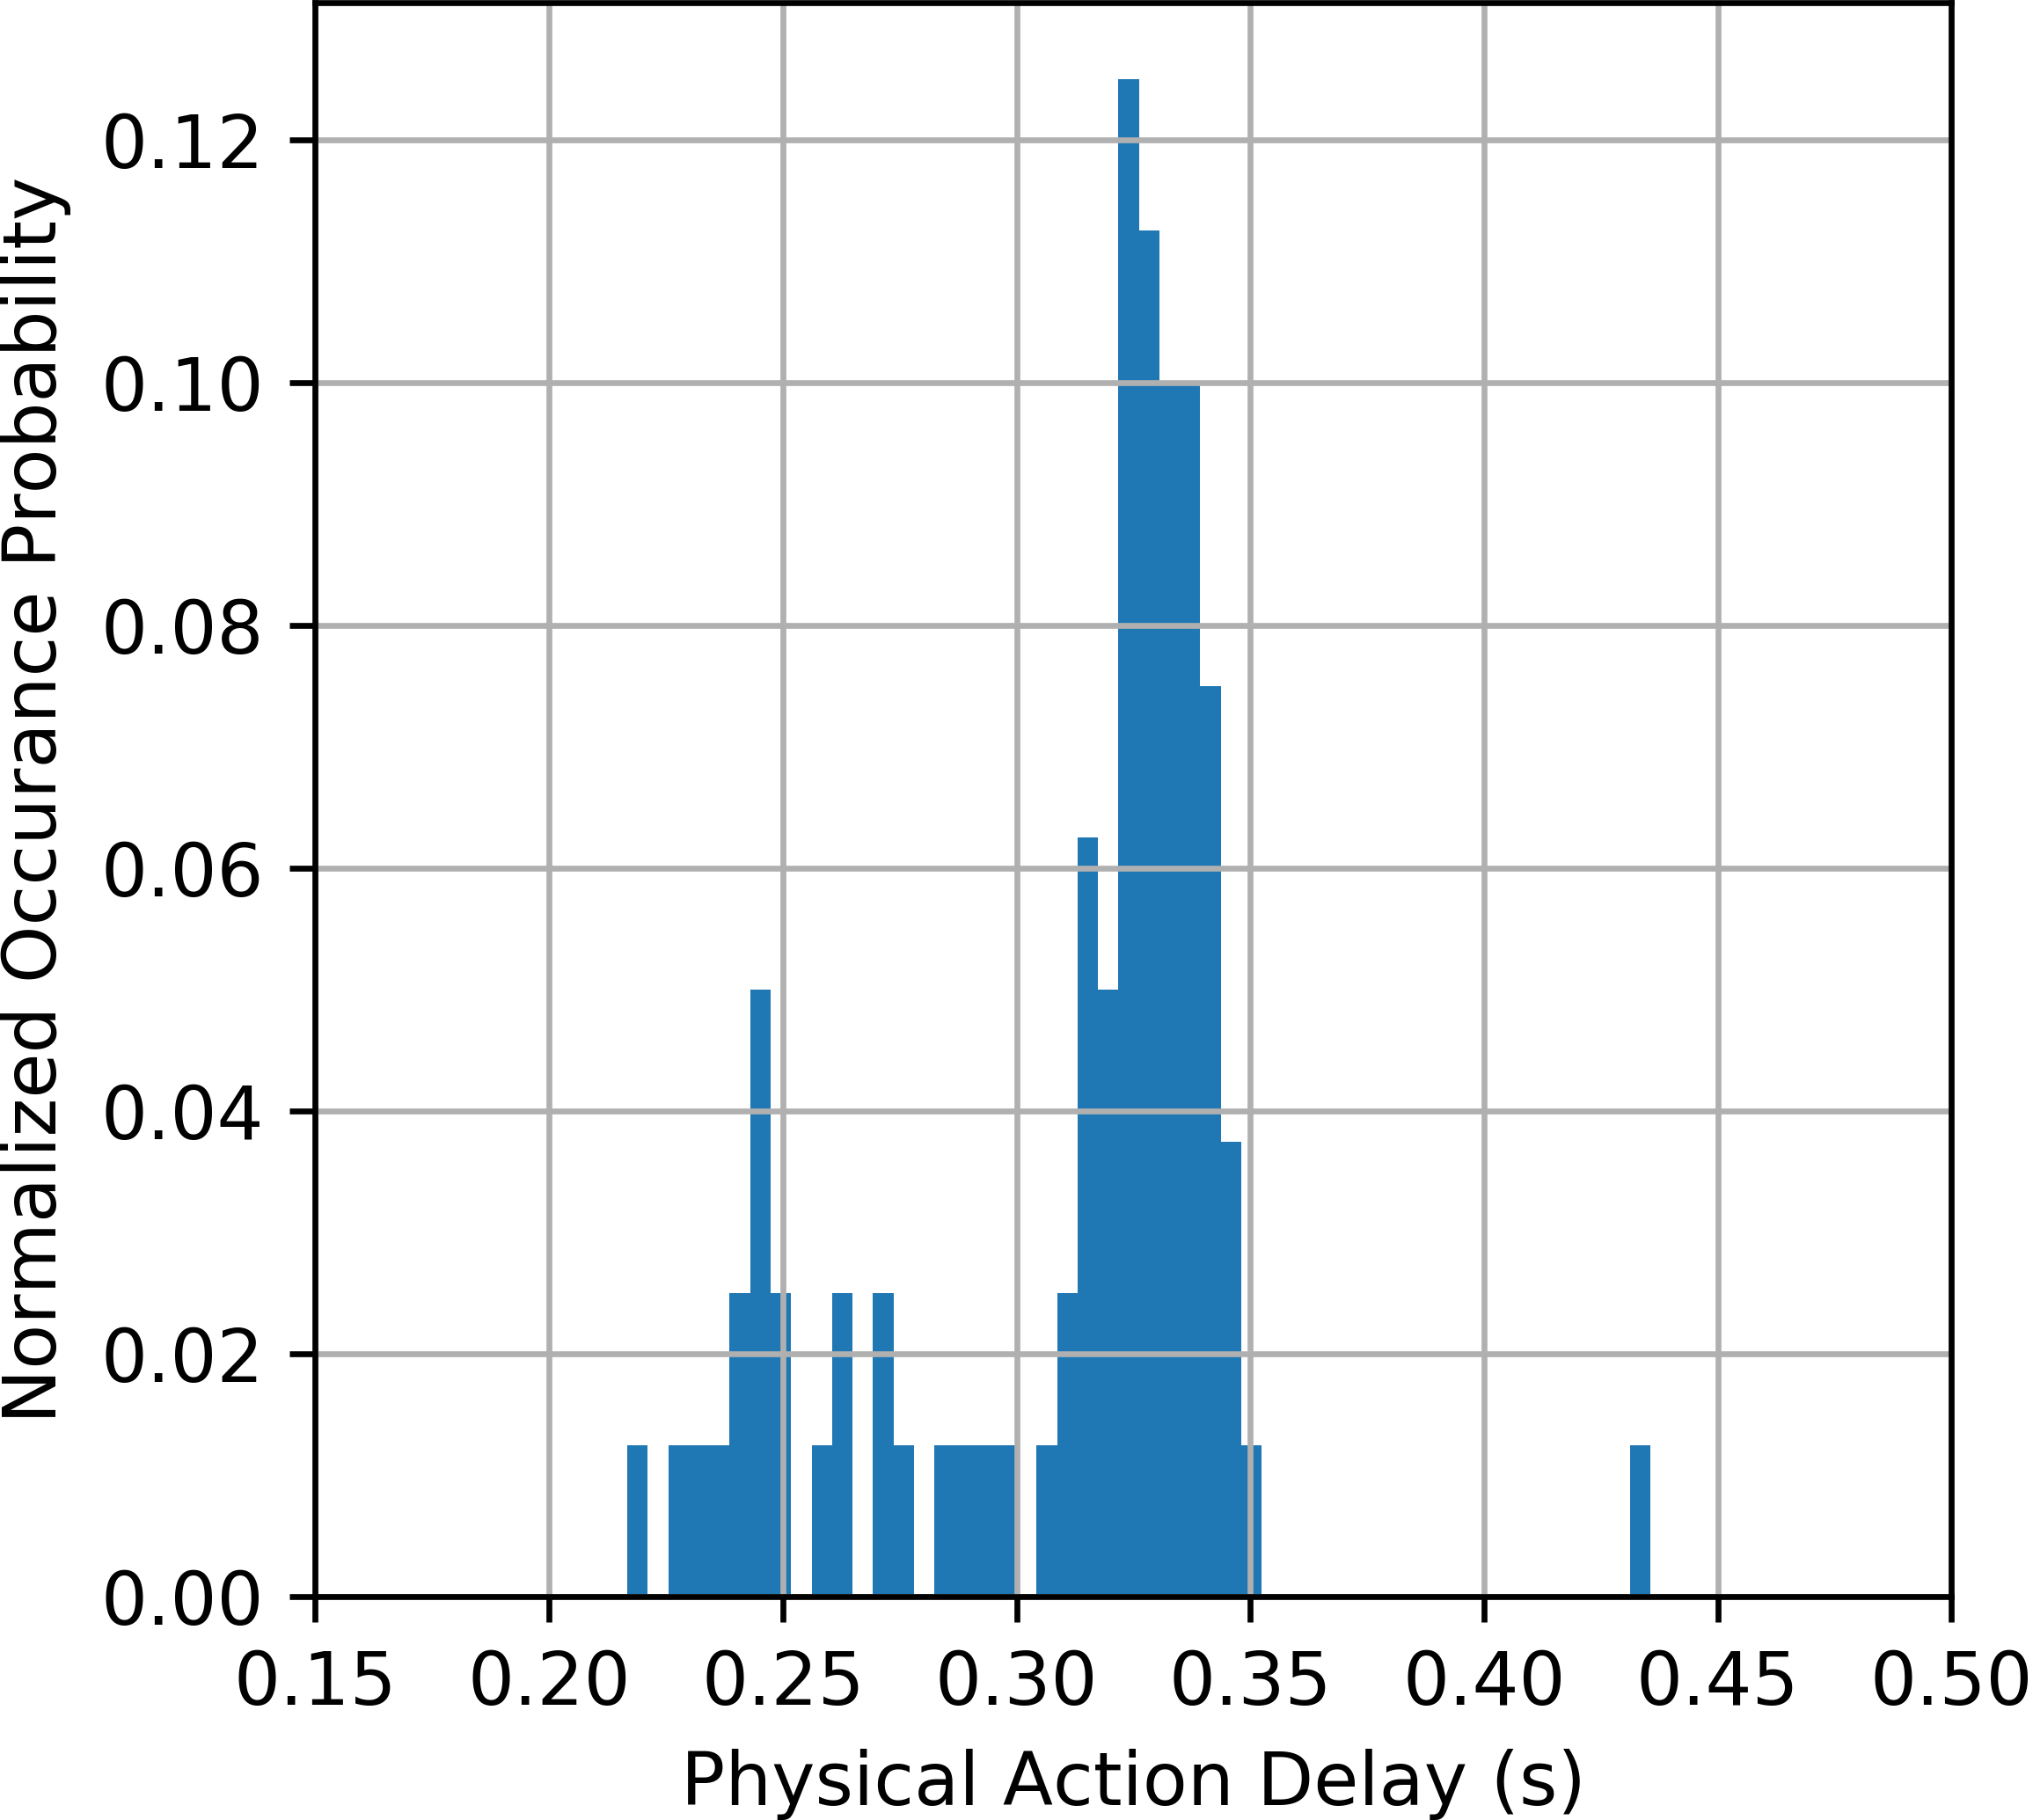
\includegraphics[width=.42\columnwidth]{chapter-gdb-appl/figures/database/WirelessBaseline_PhyHist_1.png}}\\
	\subfloat[With 2500 pps Traffic]{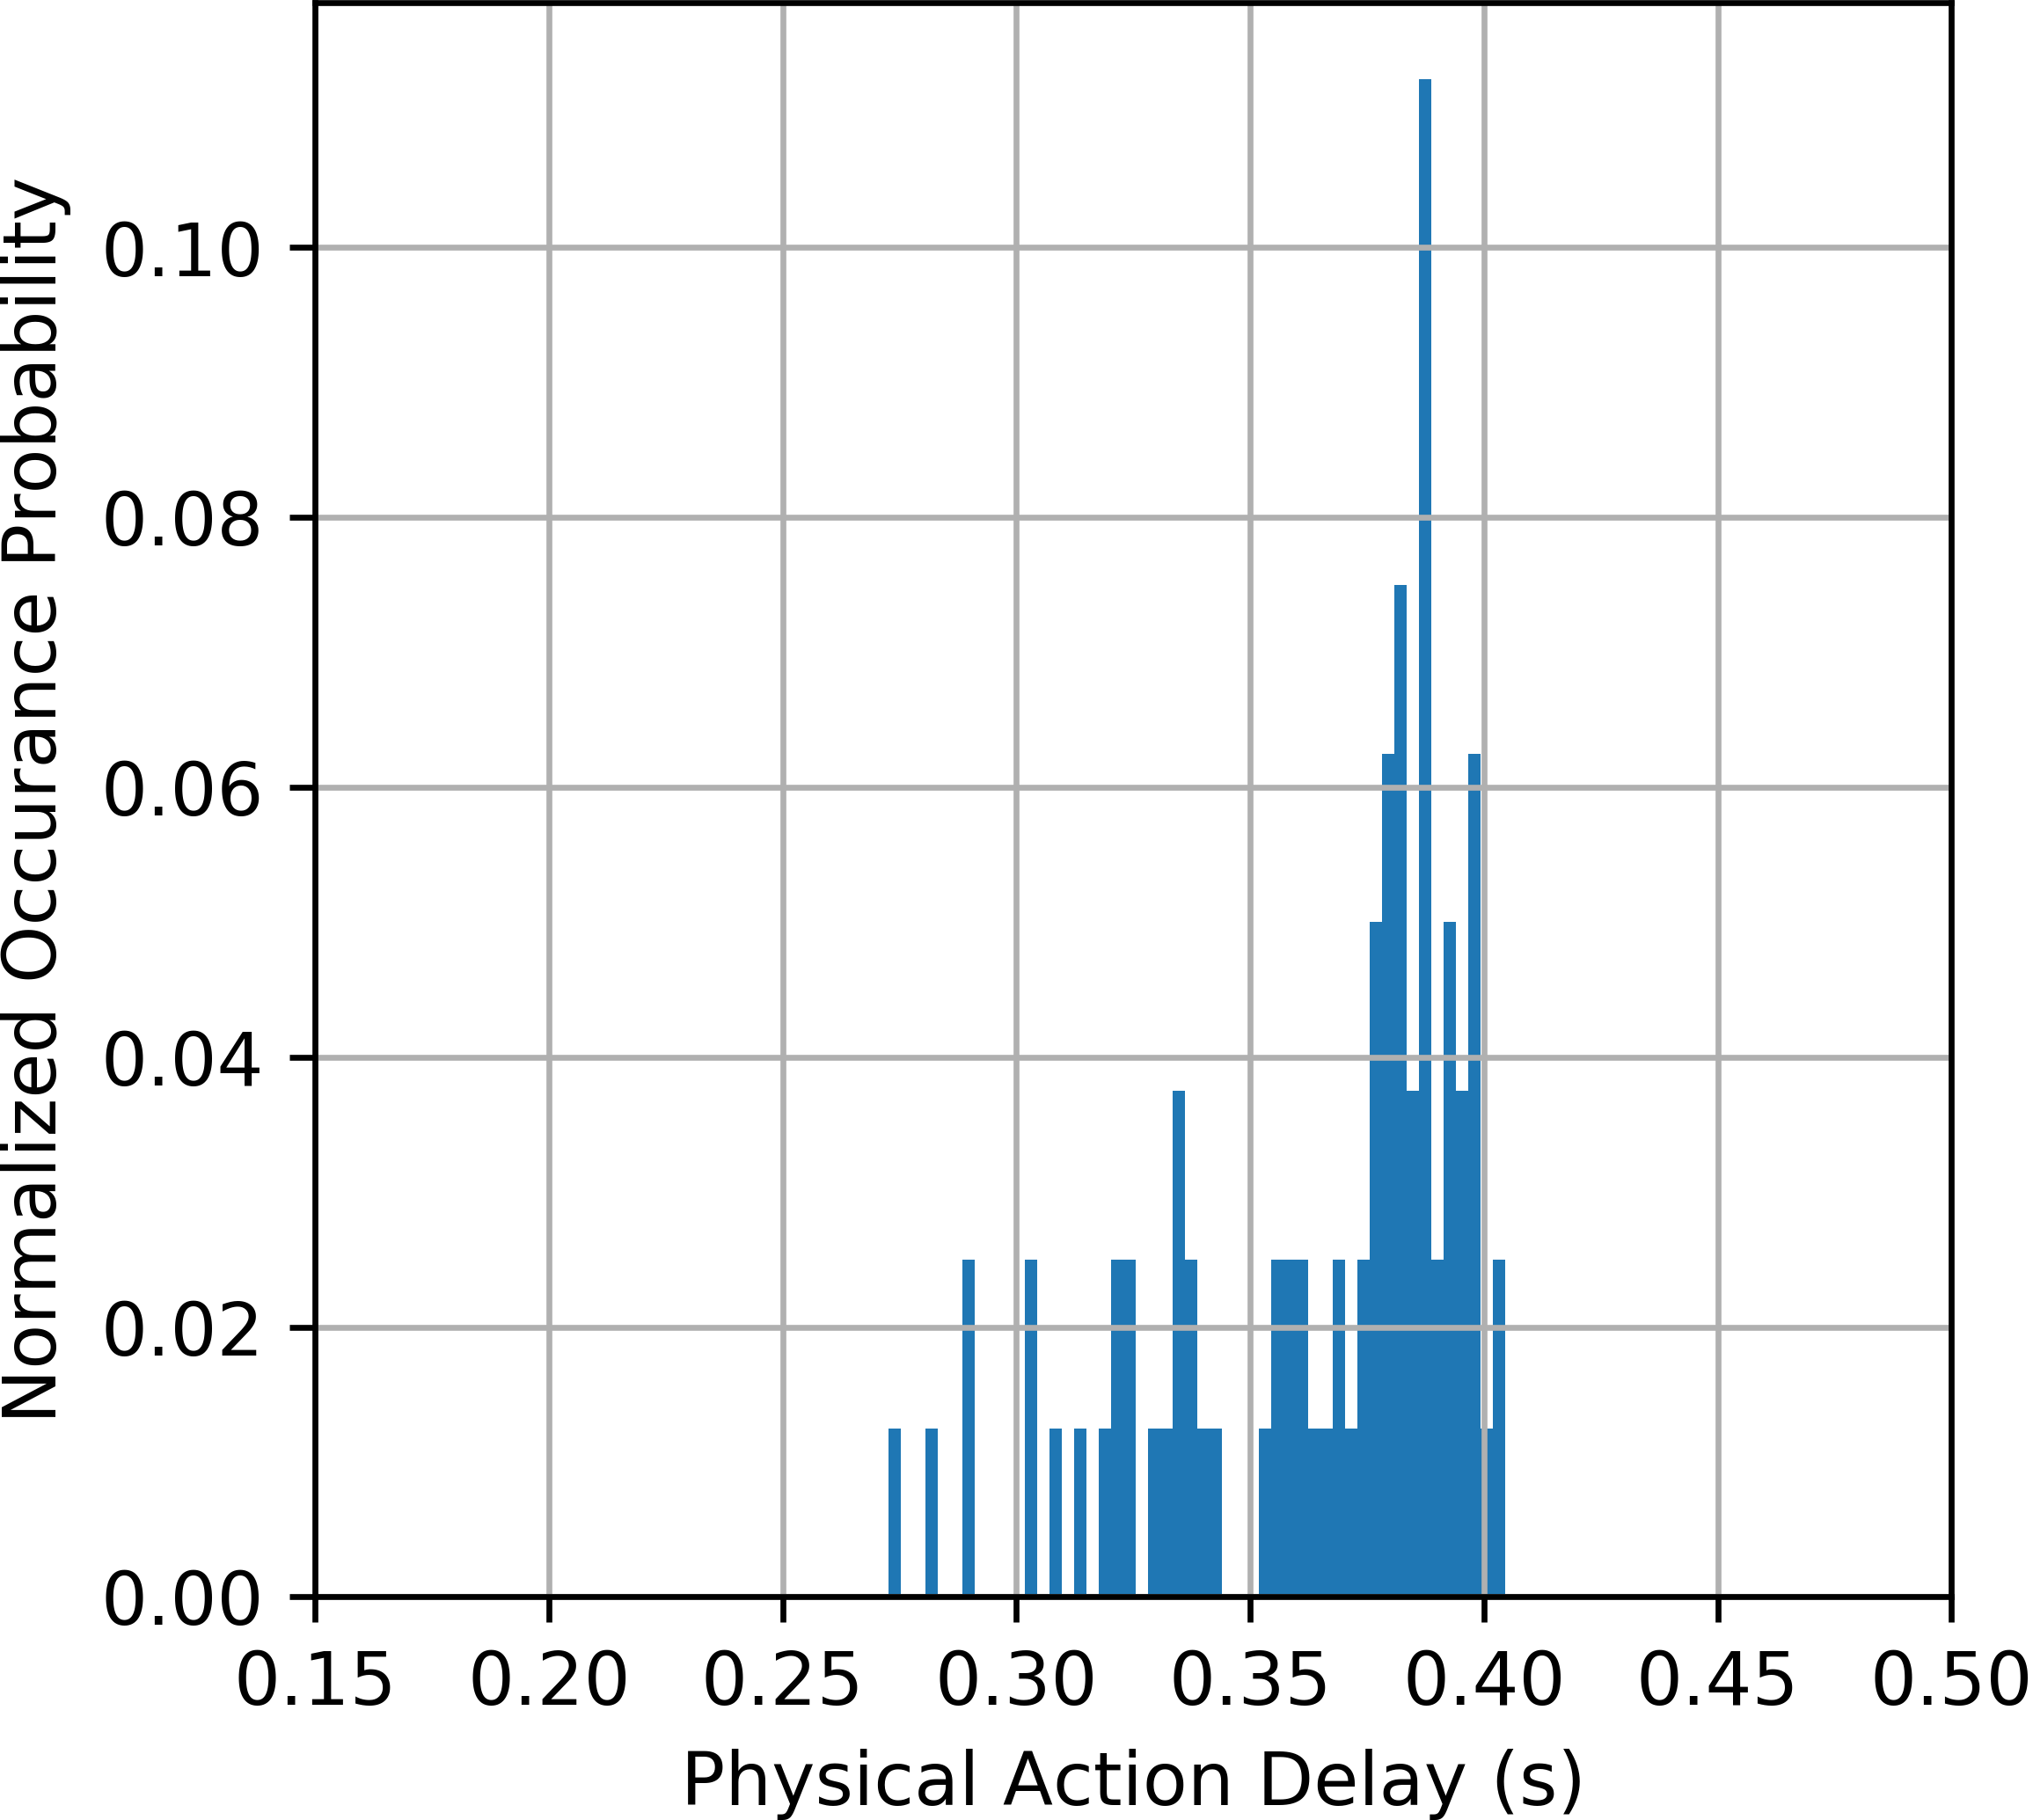
\includegraphics[width=.42\columnwidth]{chapter-gdb-appl/figures/database/2500pps1000Bv1_PhyHist_1.png}}\quad
	\subfloat[With 2x1250 pps Traffic]{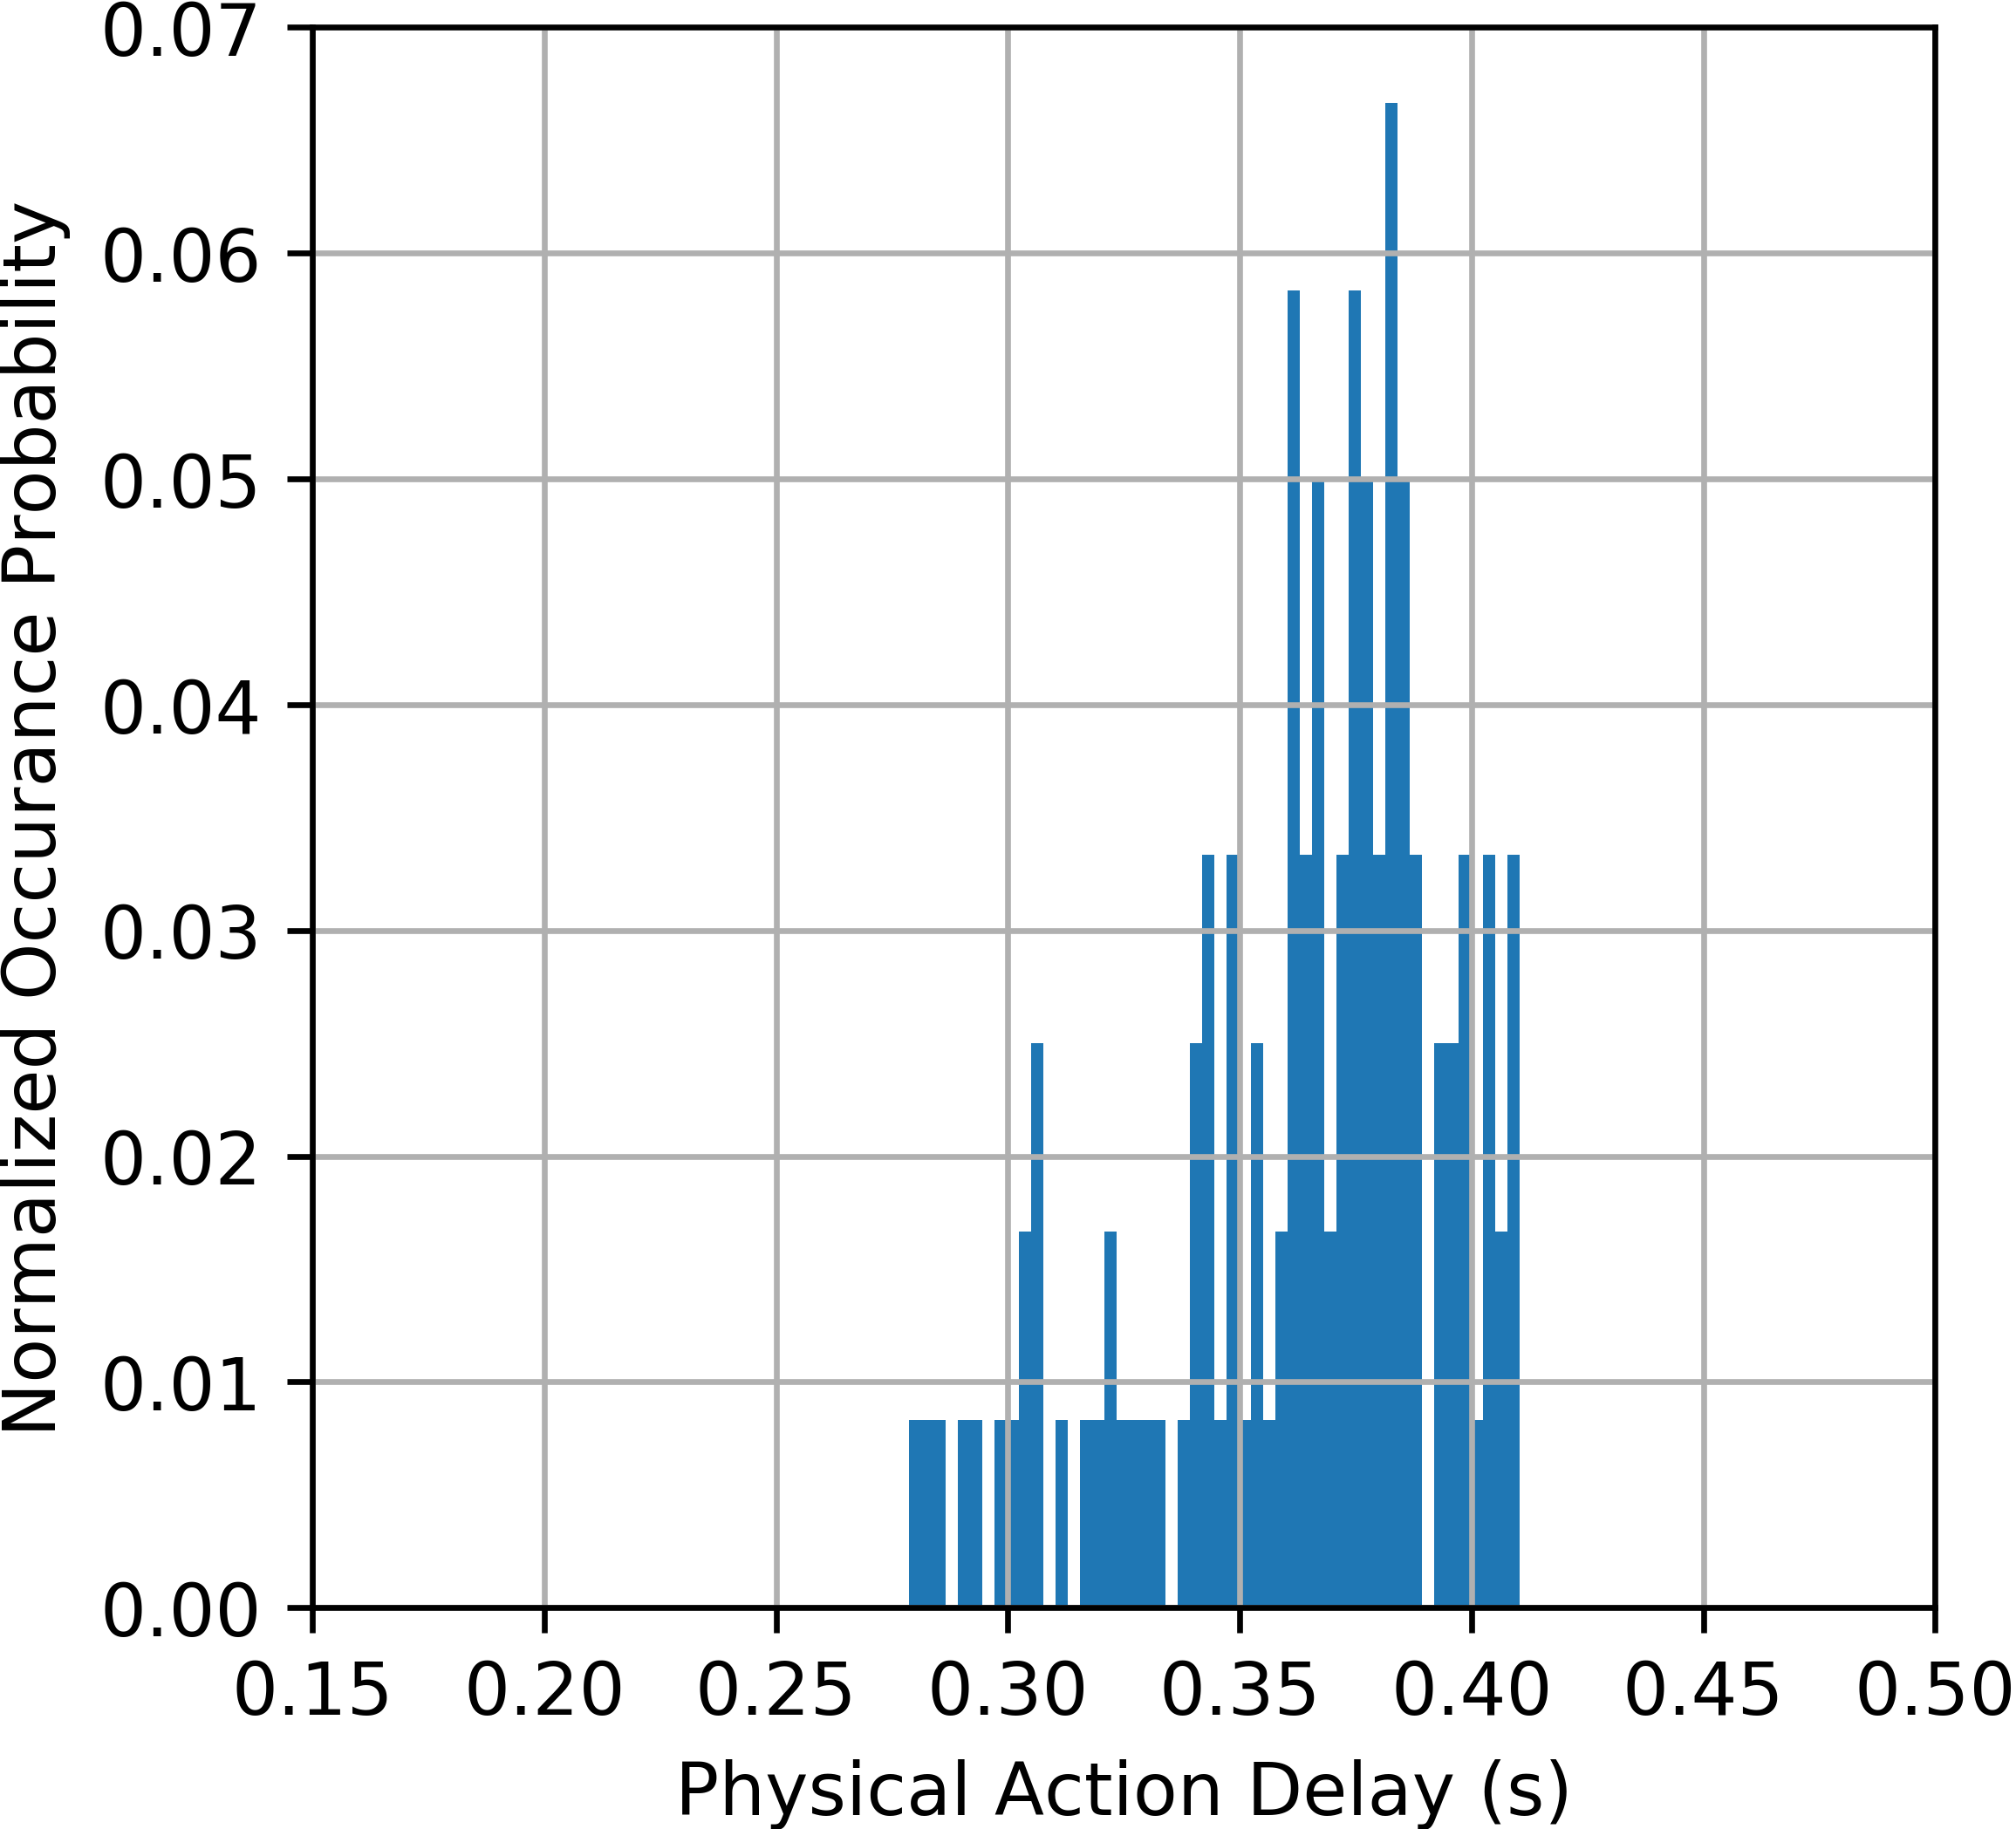
\includegraphics[width=.42\columnwidth]{chapter-gdb-appl/figures/database/2X1250pps1000Bv1_PhyHist_1.png}}
	\caption{Histograms of Action Processing Time for Various Experimental Scenarios.\vspace{-0.3in}}
	\label{gdbappl:fig:hist2}
\end{figure}


